\documentclass[12pt,a4paper,oneside]{report}
\usepackage[table]{xcolor}
\usepackage[a4paper,top=2.6cm,bottom=2.4cm,left=2.7cm,right=2.3cm]{geometry}
\usepackage[T1]{fontenc}
\usepackage[utf8]{inputenc}
\usepackage[english]{babel}
\usepackage{mathptmx}
\usepackage[scaled=0.92]{helvet}
\usepackage{graphicx}
\graphicspath{{images/}}
\usepackage{pdfpages}
\usepackage{eso-pic}
\definecolor{IITBlue}{HTML}{004389}
\definecolor{SoftBlue}{HTML}{EAF2F8}
\definecolor{Accent}{HTML}{1F497D}
\definecolor{SoftGray}{HTML}{F4F6F7}
\definecolor{DarkGray}{HTML}{3A3A3A}
\definecolor{TabHead}{gray}{0.85}
\usepackage{setspace}
\onehalfspacing
\usepackage{microtype}
\usepackage{booktabs}
\usepackage{array}
\usepackage{longtable}
\usepackage{tabularx}
\usepackage{multirow}
\usepackage{colortbl}
\usepackage{enumitem}
\usepackage{caption}
\usepackage{subcaption}
\usepackage{float}
\usepackage{fancyhdr}
\usepackage{titlesec}
\usepackage{tocloft}
\usepackage{listings}
\usepackage{tikz}
\usetikzlibrary{arrows.meta,positioning,fit,shapes.multipart,calc,shapes.geometric,shadows,chains}
\usepackage{pgfplots}
\pgfplotsset{compat=1.18}
\usepackage{hyperref}
\hypersetup{colorlinks=true, linkcolor=black, citecolor=black, urlcolor=Accent}
% Keep the table of contents concise: chapters and sections only.
\setcounter{tocdepth}{1}
\setcounter{secnumdepth}{3}
\setlength{\parindent}{0.65cm}
\setlength{\parskip}{0.20em}
\setlength{\headheight}{15pt}
\renewcommand{\arraystretch}{1.30}
\setlist[itemize]{label=\textemdash, topsep=0.25em, itemsep=0.2em, leftmargin=1.25cm}
\setlist[enumerate]{topsep=0.25em, itemsep=0.2em, leftmargin=1.25cm}
\sloppy
\hbadness=10000
\hfuzz=30pt
\vbadness=10000
\vfuzz=400pt
\emergencystretch=3em
\raggedbottom

% ---------- Content clustering: avoid orphan/widow lines and stranded headings ----------
\usepackage{needspace}
\clubpenalty=10000
\widowpenalty=10000
\displaywidowpenalty=10000
\brokenpenalty=10000
\setlength{\textfloatsep}{16pt plus 4pt minus 4pt}
\setlength{\intextsep}{16pt plus 4pt minus 4pt}
\setlength{\floatsep}{14pt plus 3pt minus 3pt}
\usepackage{etoolbox}
\pretocmd{\section}{\Needspace*{4\baselineskip}}{}{}
\pretocmd{\subsection}{\Needspace*{3\baselineskip}}{}{}

% ---------- Per-chapter Summary helper ----------
\newcommand{\chsummaryitem}[3]{\noindent\makebox[1.15cm][l]{#1}#2\,\dotfill\,\pageref{#3}\par}
\newcommand{\chsummarysub}[3]{\noindent\hspace*{1.0cm}\makebox[1.4cm][l]{#1}#2\,\dotfill\,\pageref{#3}\par}

% ---------- Running header / footer (monochrome, mirrors reference) ----------
\pagestyle{fancy}
\fancyhf{}
\fancyhead[L]{\small\rmfamily\nouppercase{}\leftmark}
\fancyfoot[L]{\small\rmfamily IIT SFAX}
\fancyfoot[R]{\small\rmfamily Page \thepage}
\renewcommand{\headrulewidth}{0.8pt}
\renewcommand{\footrulewidth}{0.6pt}
\renewcommand{\chaptermark}[1]{\markboth{\MakeUppercase{#1}}{}}
\renewcommand{\sectionmark}[1]{}
% chapter-opening / front-matter pages keep the IIT SFAX footer (mirror reference)
\fancypagestyle{plain}{%
  \fancyhf{}%
  \fancyfoot[L]{\small\rmfamily IIT SFAX}%
  \fancyfoot[R]{\small\rmfamily Page \thepage}%
  \renewcommand{\headrulewidth}{0pt}%
  \renewcommand{\footrulewidth}{0.6pt}%
}

% ---------- Caption style: FIGURE/TABLE X.Y -- text, small caps, below ----------
\DeclareCaptionLabelSeparator{dashsep}{ \textendash\ }
\captionsetup{labelsep=dashsep, labelfont={sc,bf,small}, textfont={sc,small}, justification=centering, singlelinecheck=true, skip=6pt}

% ---------- Chapter heading: black square + number + rule + title ----------
\newcommand{\chsquare}[1]{%
  {\setlength{\fboxsep}{0pt}\colorbox{black}{\parbox[c][1.15cm][c]{1.15cm}{\centering\color{white}\fontsize{30}{30}\selectfont\bfseries #1}}}%
}
\titleformat{\chapter}[display]
  {\rmfamily}
  {\normalsize\itshape Chapter\\[3pt]\chsquare{\thechapter}}
  {6pt}
  {\titlerule[1.2pt]\vspace{4pt}\raggedright\huge\bfseries}
  []
\titleformat{name=\chapter,numberless}[display]
  {\rmfamily}
  {\chsquare{\rule{0pt}{0pt}}}
  {6pt}
  {\titlerule[1.2pt]\vspace{4pt}\raggedright\huge\bfseries}
  []
\titlespacing*{\chapter}{0pt}{6pt}{18pt}

% ---------- Section headings: serif, bold, black (mirrors reference) ----------
\titleformat{\section}{\rmfamily\Large\bfseries}{\thesection}{0.6em}{}
\titleformat{\subsection}{\rmfamily\large\bfseries}{\thesubsection}{0.6em}{}
\titleformat{\subsubsection}{\rmfamily\normalsize\bfseries}{\thesubsubsection}{0.6em}{}

% ---------- Code listing style ----------
\lstdefinestyle{codeStyle}{
    basicstyle=\ttfamily\small,
    breaklines=true,
    frame=single,
    backgroundcolor=\color{SoftBlue},
    rulecolor=\color{IITBlue},
    columns=fullflexible,
    keepspaces=true,
    showstringspaces=false
}
\lstset{style=codeStyle}

\newcommand{\projecttitle}{Design and Implementation of an AI-Assisted CRM Automation Platform}
\newcommand{\shortproject}{LeadDesk}
\newcommand{\studentname}{Elissa Mezghani}
\newcommand{\university}{International Institute of Technology (IIT)}
\newcommand{\chapterintro}[1]{\vspace{0.5cm}\noindent#1\vspace{0.4cm}}
\newcommand{\figdesc}[1]{%
\vspace{-0.05cm}\noindent\small\textit{Description:} #1\par\normalsize\vspace{0.30cm}%
}
\newcommand{\screenshot}[2]{%
\begin{figure}[p]
\centering
\includegraphics[width=0.97\textwidth,height=0.78\textheight,keepaspectratio]{#1}
\caption{#2}
\end{figure}
}
% Screenshot kept together with a short interpretation paragraph right below it.
% #1 = image file, #2 = caption, #3 = interpretation sentence(s).
\newcommand{\shot}[3]{%
\begin{figure}[H]
\centering
\includegraphics[width=0.90\textwidth,height=0.66\textheight,keepaspectratio]{#1}
\caption{#2}
\end{figure}
\vspace{-0.10cm}
\noindent #3\par\vspace{0.45cm}
}

% ---- Sequence diagram styling (UML-style lifelines and messages) ----
\tikzset{
  lifehead/.style={draw=IITBlue, fill=IITBlue, text=white, rounded corners=2pt,
                   minimum width=2.5cm, minimum height=0.72cm, font=\small\bfseries, align=center},
  lifeline/.style={dashed, gray!70},
  smsg/.style={-{Latex[length=2.2mm]}, semithick, IITBlue},
  rmsg/.style={-{Latex[length=2.2mm]}, semithick, dashed, Accent},
  snote/.style={draw=Accent, fill=SoftBlue, rounded corners=2pt, font=\scriptsize,
                align=center, inner sep=2.5pt}
}
% ---- Use case diagram styling (standard UML style) ----
\definecolor{UCfill}{HTML}{FBF6DD}
\tikzset{
  uc/.style={draw=gray!65, ellipse, fill=UCfill, minimum width=3.2cm, minimum height=0.95cm,
             align=center, font=\scriptsize},
  ucsys/.style={draw=gray!70, rectangle, inner sep=14pt},
  ucedge/.style={gray!70}
}
% ---- Workflow node-flow styling ----
\tikzset{
  wfnode/.style={draw=IITBlue, fill=SoftBlue, rounded corners=2pt, align=center,
                 font=\footnotesize, minimum height=0.9cm, text width=2.5cm, inner sep=3pt},
  wfbranch/.style={draw=Accent, fill=SoftGray, rounded corners=2pt, align=center,
                 font=\footnotesize, minimum height=0.9cm, text width=2.5cm, inner sep=3pt},
  wfarr/.style={-{Latex[length=2.2mm]}, semithick, IITBlue}
}
% UML actor: stick figure with a connectable head node (#1) and a label (#3) below
\newcommand{\umlactor}[3]{%
  \node[draw, thick, circle, minimum size=6mm, inner sep=0pt] (#1) at (#2) {};
  \draw[thick] (#1.south) -- ++(0,-0.5);
  \draw[thick] ([yshift=-0.16cm]#1.south) ++(-0.33,0) -- ++(0.66,0);
  \draw[thick] ([yshift=-0.5cm]#1.south) -- ++(-0.3,-0.42);
  \draw[thick] ([yshift=-0.5cm]#1.south) -- ++(0.3,-0.42);
  \node[font=\small\bfseries] at ([yshift=-1.3cm]#1.south) {#3};
}
% Title-page full background image (applied to one page only)
\newcommand{\titlebackground}[1]{\AddToShipoutPictureBG*{\put(0,0){\includegraphics[width=\paperwidth,height=\paperheight]{#1}}}}


\begin{document}
\pagenumbering{roman}

\chapter*{Dedication}
\addcontentsline{toc}{chapter}{Dedication}
I dedicate this work to my parents and to my family, whose support gave me the motivation to continue working even during difficult phases of the project. I also dedicate this report to my teachers and supervisors, who helped me build the technical foundation needed to transform an idea into a complete application. Finally, I dedicate this work to every computer science student who is trying to build something useful, understandable, and realistic.

\clearpage
\chapter*{Acknowledgements}
\addcontentsline{toc}{chapter}{Acknowledgements}
First, I would like to express my sincere gratitude to the International Institute of Technology for the training I received during my studies in computer science. The final year project gave me the opportunity to apply many concepts learned during the program, including software architecture, web development, databases, automation, APIs, project management, and artificial intelligence.

I would also like to thank my academic and professional supervisors for their guidance and feedback. Their remarks helped me improve the technical quality of the application and the clarity of the report. I am grateful as well to the people who tested the platform and provided comments about usability, navigation, and presentation.

This project was developed step by step. At the beginning, the objective was to connect a CRM with automation workflows. Later, the work evolved into a complete operations console, with a local backend, live n8n workflows, a backend proxy, CRM automation, AI-assisted processing, and a professional interface. The experience helped me understand that a successful software project is not only about writing code, but also about explaining choices, handling errors, and creating a product that users can trust.

\clearpage
\chapter*{Abstract}
\addcontentsline{toc}{chapter}{Abstract}
Customer relationship management is a critical activity for sales teams. However, in many organizations, leads are still collected from emails, messages, phone calls, spreadsheets, and notes. This scattered process creates several problems: duplicate records, forgotten follow-ups, slow qualification, and a lack of clear visibility for managers. The objective of this final year project is to design and implement an AI-assisted CRM automation platform that helps a sales team capture leads, structure customer information, avoid duplicates, summarize CRM activity, generate follow-up messages, and interact with CRM data through an assistant.

The proposed solution is a web application called \textit{LeadDesk}. It combines a front-end operations console, a Node.js and Express backend, local persistence with NeDB, n8n workflows for automation, Odoo CRM as a business data source, and language models for controlled AI tasks. The platform runs in two execution contexts: a Local context, where the Node.js backend handles the logic and the persistence, and a Live context, where the backend forwards calls to n8n workflows. This separation keeps the platform easy to run while still allowing real CRM integration.

The project includes authentication, a CRM dashboard, lead capture, duplicate detection, a lead workspace, a follow-up center, an AI assistant, architecture documentation, settings management, and a server-side live proxy. The work was organized using an agile approach and divided into four functional sprints. This report presents the project framework, the technical study of the reusable workflow pattern, the CRM workflows and their business logic, the system architecture, the implementation sprints, the tests, the validation, the limitations, and the perspectives for future improvement.

\textbf{Keywords:} CRM, Artificial Intelligence, n8n, Odoo, Node.js, Express, Web Application, Workflow Automation, Lead Management, Final Year Project.

\clearpage
\tableofcontents
\clearpage
\listoffigures
\clearpage
\listoftables

\clearpage
\chapter*{List of Abbreviations}
\addcontentsline{toc}{chapter}{List of Abbreviations}
The table below lists the abbreviations used throughout this report.

\begin{table}[H]
\centering
\scriptsize
\resizebox{\textwidth}{!}{%
\begin{tabular}{|p{3cm}|p{11cm}|}
\hline\rowcolor{TabHead}
\textbf{Abbreviation} & \textbf{Meaning} \\
\hline
AI & Artificial Intelligence \\
\hline
API & Application Programming Interface \\
\hline
CRUD & Create, Read, Update, Delete \\
\hline
CRM & Customer Relationship Management \\
\hline
CSS & Cascading Style Sheets \\
\hline
DB & Database \\
\hline
HTTP & HyperText Transfer Protocol \\
\hline
IDE & Integrated Development Environment \\
\hline
JSON & JavaScript Object Notation \\
\hline
KPI & Key Performance Indicator \\
\hline
LLM & Large Language Model \\
\hline
MVC & Model View Controller \\
\hline
n8n & Workflow automation platform used for orchestration \\
\hline
NeDB & Embedded JavaScript database used for local persistence \\
\hline
Odoo & ERP and CRM platform used as the system of record \\
\hline
PFE & Projet de Fin d'Etudes / Final Year Project \\
\hline
REST & Representational State Transfer \\
\hline
SaaS & Software as a Service \\
\hline
UI & User Interface \\
\hline
UX & User Experience \\
\hline
\end{tabular}%
}
\end{table}

\cleardoublepage
\pagenumbering{arabic}
\chapter*{General Introduction}
\addcontentsline{toc}{chapter}{General Introduction}
\markboth{GENERAL INTRODUCTION}{GENERAL INTRODUCTION}
Customer relationship management is an important part of the sales process. A lead can arrive through an email, a phone call, a contact form, or a direct message. The sales employee then has to understand the request, copy the customer information, check if the lead already exists, and prepare the next action. When this work is done manually, small mistakes can appear. A phone number can be written incorrectly, the same customer can be created twice, or an interested prospect can be forgotten.

This final year project answers this problem by proposing an AI-assisted CRM automation platform. The goal is not to replace Odoo CRM, but to add a simple operational layer that helps the user work faster and with better data quality. The platform allows the user to capture leads from natural messages, detect duplicate records, create or inspect opportunities, generate CRM summaries, prepare follow-up messages, and ask questions through an assistant connected to CRM data.

The application is built with a web interface, a Node.js and Express backend, n8n workflows, Odoo CRM, and AI models. The web interface gives the user a clear place to manage CRM actions. The backend handles authentication, API requests, and communication with the automation layer. The n8n workflows execute the business logic and connect the platform with Odoo CRM. AI is used only where it adds value, such as text extraction, summarization, follow-up writing, and conversational assistance.

This report is organized as a final year project book. The first chapter presents the project framework, the existing situation, the problem statement, the comparative study, the methodology, the needs analysis, and the proposed solution. The second chapter presents the technical study, including the development environment, the tools used, the workflow study, and the conceptual design. The following chapters present the implementation sprints, the workflow diagrams, the tests, the validation, the limitations, and the possible improvements.

\chapter{Project Framework}

\vspace{0.35cm}
{\Large\bfseries Summary}\par
\vspace{3pt}{\color{black}\hrule height 0.6pt}\vspace{0.30cm}
{\small
\chsummaryitem{1.1}{Introduction}{sumlbl:c1s1}
\chsummaryitem{1.2}{Host Company: Connexant}{sumlbl:c1company}
\chsummaryitem{1.3}{Problem Statement}{sumlbl:c1s2}
\chsummaryitem{1.4}{Existing Situation}{sumlbl:c1s3}
\chsummaryitem{1.5}{Comparative Study}{sumlbl:c1s4}
\chsummaryitem{1.6}{Needs Analysis: EPICs and User Stories}{sumlbl:c1s5}
\chsummaryitem{1.7}{Proposed Solution}{sumlbl:c1s6}
\chsummaryitem{1.8}{Adopted Methodology: Scrum}{sumlbl:c1s7}
\chsummaryitem{1.9}{Conclusion}{sumlbl:c1s8}
}
\clearpage



\section{Introduction}\label{sumlbl:c1s1}
Understanding the general framework of a project is necessary before presenting the technical implementation. This chapter explains the context in which the project was developed, the problems observed in classical CRM management, and the reasons that motivated the creation of an AI-assisted platform. It also introduces the methodology, the user needs, and the proposed solution at a functional level.

\section{Host Company: Connexant}\label{sumlbl:c1company}

\begin{figure}[H]
\centering
\includegraphics[width=0.50\textwidth]{connexant-logo.png}
\caption{Connexant company logo}
\label{fig:connexant-logo}
\end{figure}
\figdesc{The logo identifies Connexant, the host company whose IT consulting and infrastructure environment frames this project.}

Connexant is an information technology company operating in the computer networking products sector. Its activities combine software-solution development with consulting in IT infrastructure, which provides a relevant professional setting for a CRM automation project. The company profile highlights more than ten years of experience in IT and project leadership across energy, healthcare, finance, agriculture, and cybersecurity.

The profile also reflects a strong emphasis on professional standards and infrastructure expertise. It includes ISO 27001 auditor and IRCA credentials, certifications related to Linux, Cisco, and Novell products, and Project Management Professional (PMP) certification. It further notes third-party auditing work for SGS concerning the ISO 9001 and ISO 27001 standards. This combination of technical consulting, project management, and information-security experience makes process reliability, traceability, and controlled automation particularly important in the company's work.

Within this context, the project contributes an operational layer for CRM work. It focuses on structured lead capture, duplicate prevention, opportunity monitoring, follow-up preparation, and reliable access to CRM information. These functions align with Connexant's technology-oriented environment and with the need to manage business relationships through clear, repeatable processes. The company's website is listed in the Webography at the end of the report.

\section{Problem Statement}\label{sumlbl:c1s2}
In the current sales process, a lead can arrive as a simple message, a phone call note, an email, a form submission, or as an officially routed prospect through the Odoo Partner Program, but the useful information is not always ready to be used inside the CRM. The sales employee has to read the message, understand what the customer wants, copy the name, phone number, email, and interest, then check manually if this person already exists before creating a new opportunity. This daily work may seem simple, but it easily becomes a source of mistakes: a phone number can be written incorrectly, a customer can be added twice, an old lead can be forgotten, and the manager may not have a clear view of which opportunities need attention first. These small problems directly affect the quality of follow-up and can make the company lose time and potential customers. The problem addressed in this project is therefore the lack of a simple and reliable layer that helps the sales team structure incoming lead information, avoid repeated records, detect inactive opportunities, and make CRM data easier to understand and use.

\section{Existing Situation}\label{sumlbl:c1s3}
Today, a sales team handles its leads either by hand or with a standard CRM. This project is built on Odoo CRM. According to the official Odoo documentation~\textup{[W1]}, Odoo CRM helps a team organize its sales activities: it tracks leads, closes opportunities, gives accurate forecasts, and keeps opportunities organized in a pipeline with meetings and next activities. Odoo is therefore a solid system of record for the customer data.

However, Odoo on its own does not read a free-text customer message, does not draft a follow-up, and does not answer questions in natural language; these steps stay manual. The same limit applies to the other tools a team might use instead. To position the project clearly, the next section defines the main existing solutions and compares them with the proposed platform.



\section{Comparative Study}\label{sumlbl:c1s4}
Before comparing the proposed solution with the existing approaches, this section first defines the existing solutions, then positions the proposed platform against them.

\subsection{Existing Solutions}\label{sumlbl:c1s4ss1}
Three approaches are commonly used by a sales team to manage its leads before adopting a dedicated tool like the one built in this project.

\begin{itemize}
\item \textbf{Spreadsheet.} Spreadsheets are simple online tools that help users organize information in rows and columns. Google Sheets is a common example used to maintain basic sales records.~\textup{[W2]}
\item \textbf{Standard CRM.} CRM stands for customer relationship management, which is a system for managing an organization's interactions with current and potential customers.~\textup{[W3]}
\item \textbf{Automation-only tool.} An automation tool is software that takes over repetitive tasks, connects systems, and ensures that a flow is carried out consistently. It can create records, move data between systems, send notifications, perform rule-based checks, flag deviations, and trigger the next step in a process.~\textup{[W4]}
\end{itemize}

\subsection{Our Solution Compared with the Existing Solutions}\label{sumlbl:c1s4ss2}
The \textbf{proposed LeadDesk} is the solution built in this project. It is an operations console that adds AI-assisted lead capture, duplicate control, analytics, and a CRM assistant on top of Odoo CRM and n8n workflows. The aim is not to replace a CRM, but to add an operational layer that the existing solutions do not provide on their own.

The table below compares the proposed platform with the three existing solutions on the points that matter most for daily CRM work.

\begin{table}[H]
\centering
\scriptsize
\setlength{\tabcolsep}{3pt}
\begin{tabularx}{\textwidth}{|p{2.6cm}|p{1.9cm}|p{1.9cm}|p{2.0cm}|X|}
\hline\rowcolor{TabHead}
\textbf{Feature} & \textbf{Spreadsheet}\newline(Excel, Sheets) & \textbf{Standard CRM}\newline(Odoo, Salesforce) & \textbf{Automation only}\newline(n8n, Zapier) & \textbf{Proposed platform} \\
\hline
Centralized records & Weak & Strong & Depends on integration & Strong through CRM and local store \\
\hline
Lead extraction from text & No & Manual & Limited & Yes, through controlled AI prompts \\
\hline
Duplicate prevention & Manual & Partial & Possible & Explicit email and phone check \\
\hline
Inactive lead detection & No & Manual & Possible with rules & Automatic after seven days \\
\hline
Manager summary & Manual & Reports & Rule-based & KPI calculation plus readable summary \\
\hline
Follow-up drafting & Manual & Manual templates & Templates & Personalized AI-assisted messages \\
\hline
Runs locally without cloud setup & Yes & Usually no & Usually no & Yes, local Node.js backend \\
\hline
Natural-language assistant & No & Rare or paid & No & Yes, tool-based assistant \\
\hline
\end{tabularx}
\caption{Comparison between the existing approaches and the proposed solution}
\end{table}

\section{Needs Analysis: EPICs and User Stories}\label{sumlbl:c1s5}
The needs were divided into EPICs and user stories in order to make the project easier to plan and validate. The EPICs represent large functional areas, while user stories describe concrete needs from the point of view of a user or the system. This structure also makes the report closer to a professional software engineering document.


The table below lists the main user stories of the project, grouped by EPIC.

\begin{table}[H]
\centering
\small
\begin{tabularx}{\textwidth}{|p{1.5cm}|p{3.2cm}|X|p{2cm}|}
\hline\rowcolor{TabHead}
\textbf{ID} & \textbf{EPIC} & \textbf{User Story} & \textbf{Priority} \\
\hline
US-01 & Authentication & As a user, I want to sign in securely so that I can access CRM operations. & Critical \\
\hline
US-02 & Lead Capture & As a sales employee, I want to paste a customer message so that the system extracts useful CRM fields. & Critical \\
\hline
US-03 & Data Quality & As a sales employee, I want duplicate detection so that I do not create repeated opportunities. & Critical \\
\hline
US-04 & Analytics & As a manager, I want clear KPIs so that I can understand the pipeline quickly. & High \\
\hline
US-05 & Follow-up & As a sales employee, I want inactive leads to be identified so that I can contact them again. & High \\
\hline
US-06 & AI Assistant & As a user, I want to ask CRM questions in natural language so that I can retrieve information faster. & High \\
\hline
US-07 & Live Integration & As a user, I want the platform to call real n8n workflows when needed. & High \\
\hline
\end{tabularx}
\caption{Backlog of main user stories}
\end{table}
\section{Proposed Solution}\label{sumlbl:c1s6}
The proposed solution is an operations console named LeadDesk. It is designed as a bridge between the sales operator and the CRM automation system. The user interacts with a simple web interface. The interface runs locally through the Node.js backend and connects to the live n8n workflows when real CRM actions are needed. The workflows then communicate with Odoo CRM and AI models.

The solution is organized into three layers. The presentation layer contains the web interface and the user experience. The backend layer exposes API routes, manages authentication, stores local data, and proxies live calls. The automation and CRM layer contains n8n workflows, Odoo CRM records, and the language models. This separation improves maintainability because each layer has a clear responsibility.


The figure below presents the simplified architecture of the proposed solution and its three layers.

\begin{figure}[H]
\centering
\resizebox{0.95\textwidth}{!}{%
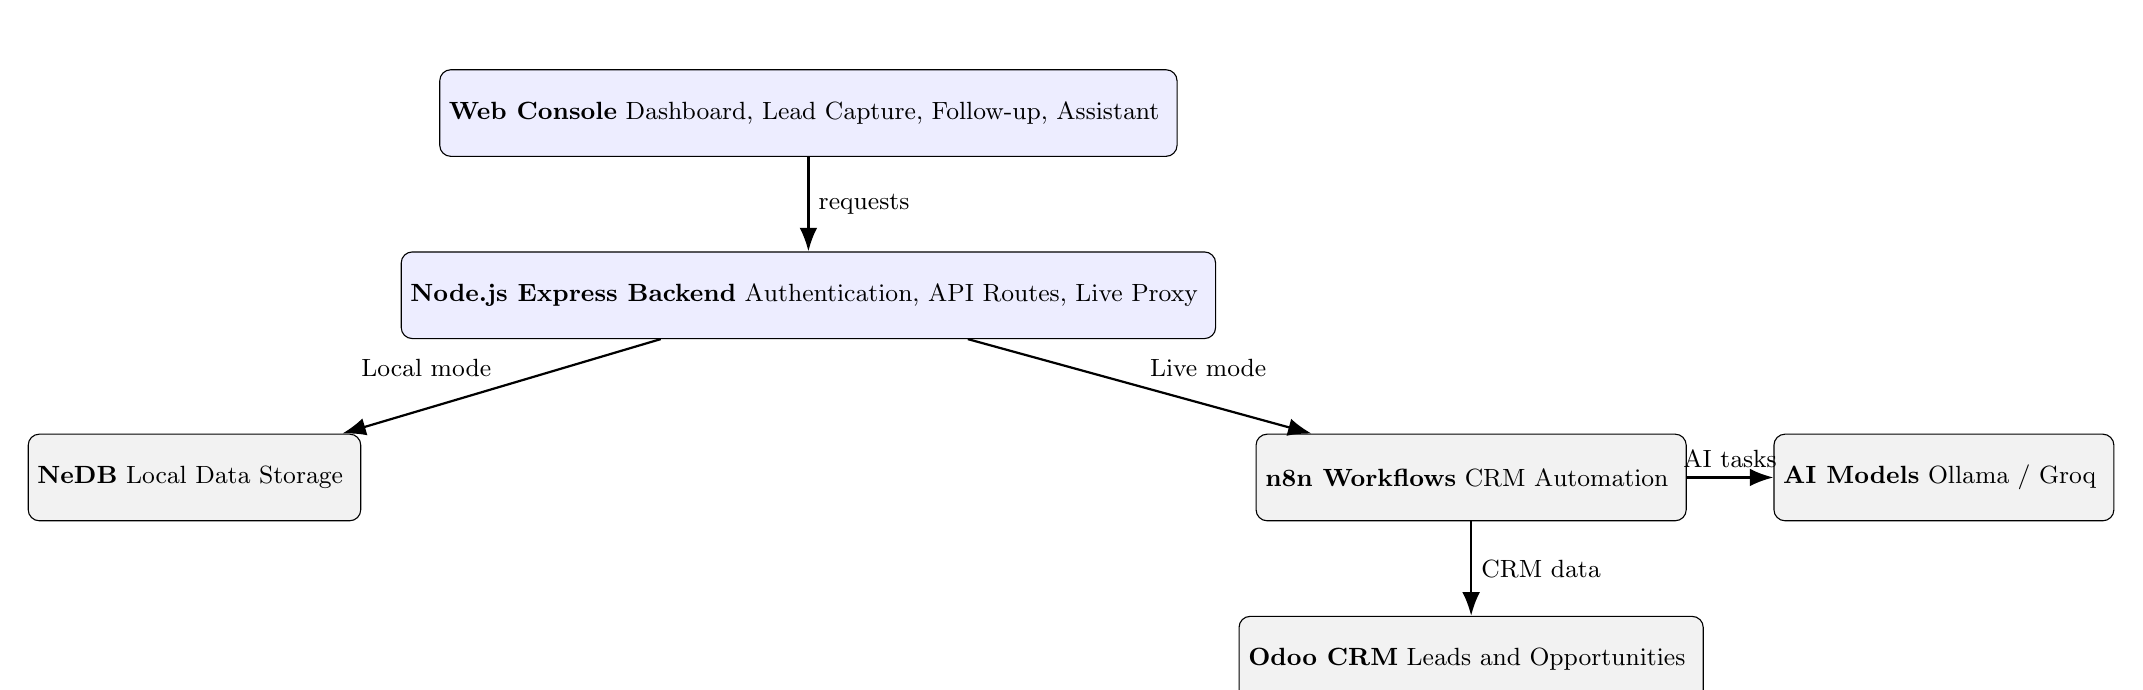
\begin{tikzpicture}[
node distance=1.2cm,
every node/.style={font=\small},
layer/.style={
draw,
rounded corners,
minimum width=5.2cm,
minimum height=1.1cm,
align=center,
fill=blue!7
},
side/.style={
draw,
rounded corners,
minimum width=4.2cm,
minimum height=1.1cm,
align=center,
fill=gray!10
},
arrow/.style={-{Latex[length=3mm]}, thick}
]

% Main layers
\node[layer] (frontend) {
\textbf{Web Console}\
Dashboard, Lead Capture, Follow-up, Assistant
};

\node[layer, below=of frontend] (backend) {
\textbf{Node.js Express Backend}\
Authentication, API Routes, Live Proxy
};

\node[side, below left=1.2cm and 0.5cm of backend] (nedb) {
\textbf{NeDB}\
Local Data Storage
};

\node[side, below right=1.2cm and 0.5cm of backend] (n8n) {
\textbf{n8n Workflows}\
CRM Automation
};

\node[side, below=of n8n] (odoo) {
\textbf{Odoo CRM}\
Leads and Opportunities
};

\node[side, right=1.1cm of n8n] (ai) {
\textbf{AI Models}\
Ollama / Groq
};

% Arrows
\draw[arrow] (frontend) -- node[right]{requests} (backend);
\draw[arrow] (backend) -- node[above left]{Local mode} (nedb);
\draw[arrow] (backend) -- node[above right]{Live mode} (n8n);
\draw[arrow] (n8n) -- node[right]{CRM data} (odoo);
\draw[arrow] (n8n) -- node[above]{AI tasks} (ai);

\end{tikzpicture}%
}
\caption{Simplified architecture of the proposed LeadDesk}
\label{fig:global-architecture}
\end{figure}
\figdesc{The diagram shows how the web console sends requests to the backend, which uses NeDB for local operations or n8n, Odoo CRM, and AI models for live operations.}


\section{Adopted Methodology: Scrum}\label{sumlbl:c1s7}
\subsection{Scrum Presentation}\label{sumlbl:c1s7ss1}
It starts with understanding the Scrum framework which is defined in The Scrum Guide and was first introduced to the world in 1995 as a better way of team collaboration for solving complex problems.  The Scrum framework is fairly simple being made up of a Scrum Team consisting of a Product Owner, a Scrum Master and Developers, each of which have specific accountabilities. The Scrum Team takes part in five events and produces three artifacts. Scrum co-creators Ken Schwaber and Jeff Sutherland wrote and maintain The Scrum Guide, which explains Scrum clearly and succinctly.  The guide contains the definition of Scrum,  describing the Scrum accountabilities, events, artifacts and the guidance that binds them together.

Scrum is an empirical process, where decisions are based on observation, experience and experimentation. Scrum has three pillars: transparency, inspection and adaptation. This supports the concept of working iteratively. Empiricism means working through small experiments, learning from that work, and adapting both the work itself and the way it is performed.~\textup{[W5]}

The figure below illustrates the Scrum framework and its main elements.

\begin{figure}[H]
\centering
\resizebox{0.96\textwidth}{!}{%
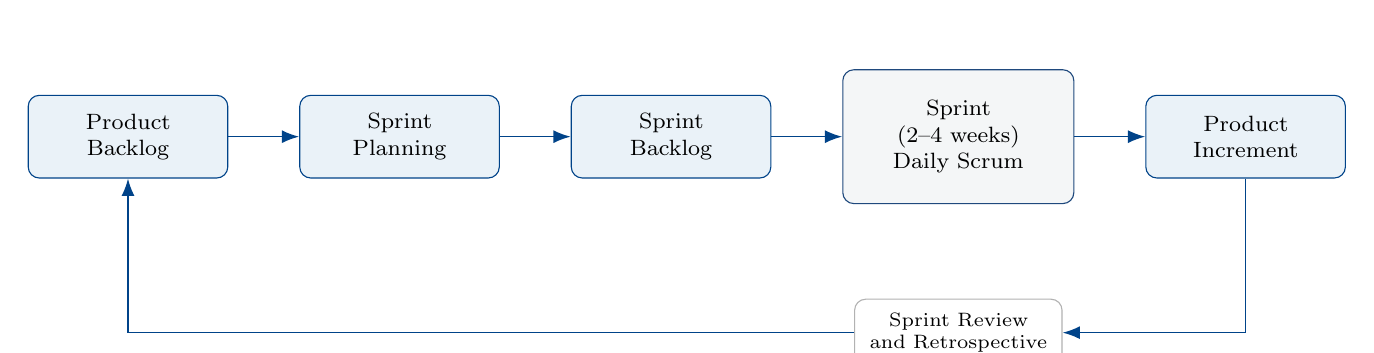
\begin{tikzpicture}[node distance=9mm, >={Latex[length=2.4mm]},
  sb/.style={draw=IITBlue, fill=SoftBlue, rounded corners, align=center, font=\footnotesize, minimum height=1.05cm, text width=2.3cm},
  sprint/.style={draw=Accent, fill=SoftGray, rounded corners, align=center, font=\footnotesize, minimum height=1.7cm, text width=2.7cm},
  ev/.style={draw=gray!60, fill=white, rounded corners, align=center, font=\scriptsize, minimum height=0.85cm, text width=2.4cm}]
\node[sb] (pb) {Product\\Backlog};
\node[sb, right=of pb] (plan) {Sprint\\Planning};
\node[sb, right=of plan] (sbk) {Sprint\\Backlog};
\node[sprint, right=of sbk] (sp) {Sprint\\(2--4 weeks)\\Daily Scrum};
\node[sb, right=of sp] (inc) {Product\\Increment};
\node[ev, below=12mm of sp] (rev) {Sprint Review\\and Retrospective};
\draw[wfarr] (pb) -- (plan);
\draw[wfarr] (plan) -- (sbk);
\draw[wfarr] (sbk) -- (sp);
\draw[wfarr] (sp) -- (inc);
\draw[wfarr] (inc) |- (rev);
\draw[wfarr] (rev) -| (pb);
\end{tikzpicture}%
}
\caption{Scrum framework}
\label{fig}
\end{figure}
\figdesc{The diagram presents the recurring Scrum cycle from backlog planning through the sprint, product increment, review, and retrospective.}


\subsection{Agile Project Breakdown}\label{sumlbl:c1s7ss2}

The table below summarizes how the project was divided into four functional sprints.

\begin{table}[H]
\centering
\begin{tabularx}{\textwidth}{|p{3cm}|X|X|}
\hline\rowcolor{TabHead}
\textbf{Sprint} & \textbf{Main objective} & \textbf{Main deliverables} \\
\hline
Sprint 1 & Platform foundation & Interface structure, navigation, authentication, local dataset \\
\hline
Sprint 2 & Lead capture & Extraction, duplicate detection, opportunity creation, capture history \\
\hline
Sprint 3 & Analytics and follow-up & KPI dashboard, summary, inactive lead detection, follow-up drafts \\
\hline
Sprint 4 & Assistant and live mode & AI assistant, n8n webhooks, backend proxy, settings, tests \\
\hline
\end{tabularx}
\caption{Agile decomposition of the project into functional sprints}
\end{table}

The Gantt chart below shows the planned schedule of the project across the sprints.
\begin{figure}[H]
\centering
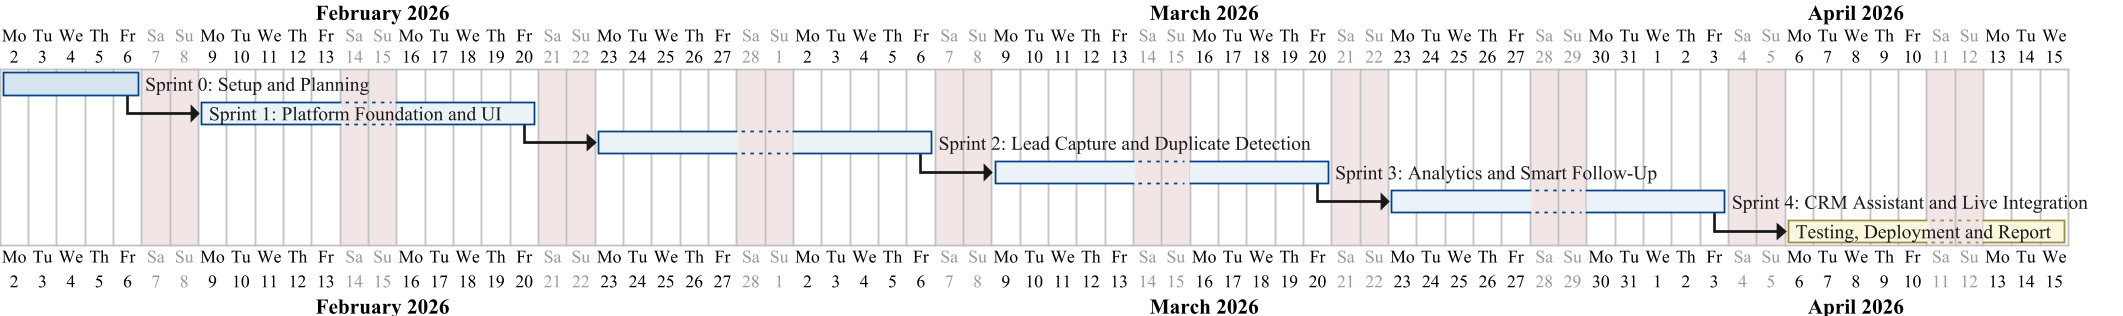
\includegraphics[width=\textwidth,height=0.5\textheight,keepaspectratio]{umls/img/gantt-project.png}
\caption{Project schedule (Gantt chart)}
\label{fig:gantt}
\end{figure}
\figdesc{The Gantt chart places the project activities on a shared timeline and shows how the four sprints follow one another.}


The work breakdown structure below decomposes the project into its main work packages.
\begin{figure}[H]
\centering
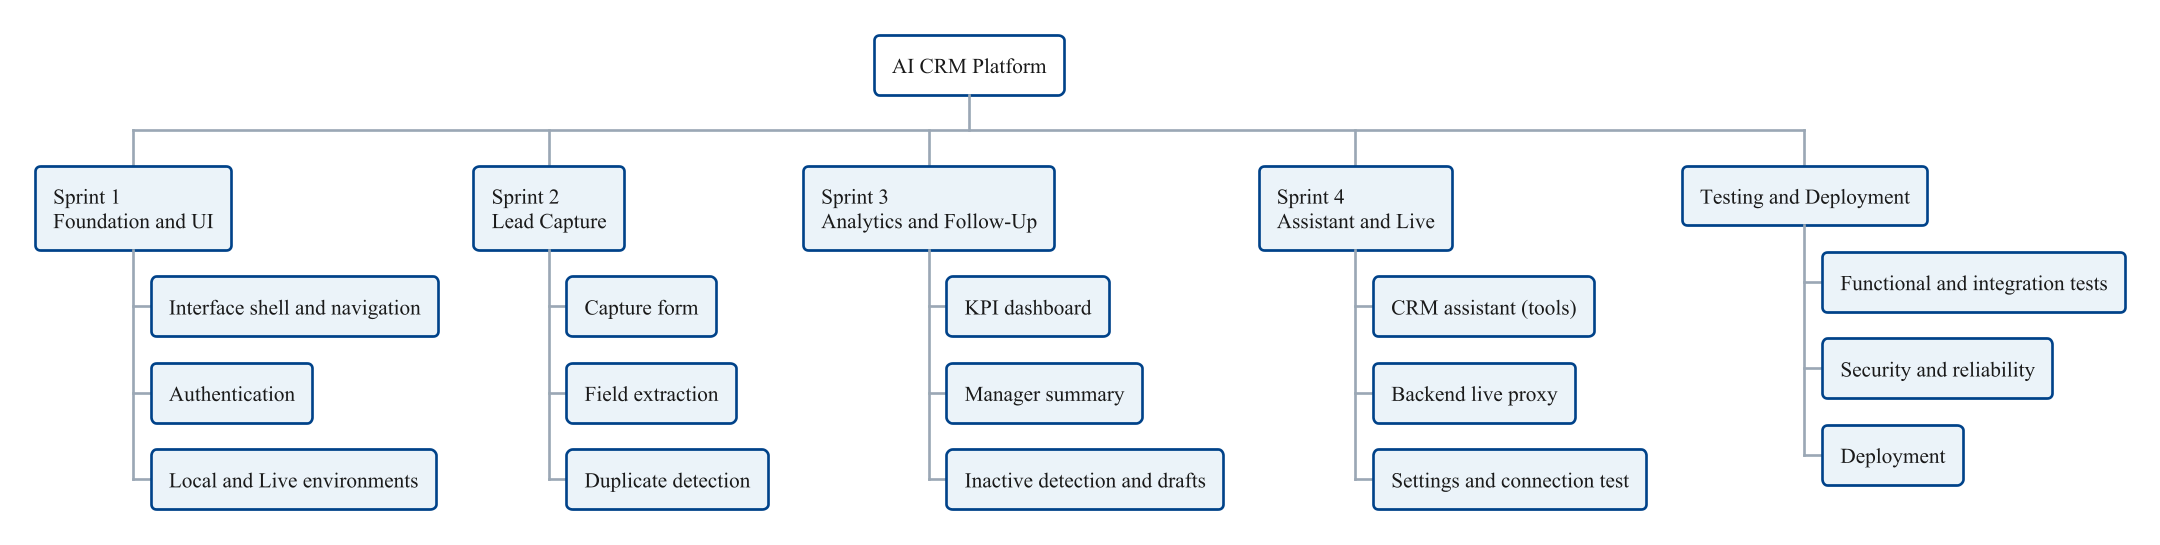
\includegraphics[width=\textwidth,height=0.55\textheight,keepaspectratio]{umls/img/wbs-project.png}
\caption{Work breakdown structure of the project}
\label{fig:wbs}
\end{figure}
\figdesc{The work breakdown structure decomposes the project into manageable work packages covering preparation, implementation, integration, testing, and documentation.}

\section{Conclusion}\label{sumlbl:c1s8}
This chapter introduced the project context, the main problems, the methodology, the needs, and the proposed solution. The next chapter focuses on a specific aspect of the project that is very important in workflow-based systems: repeated nodes and reusable patterns. Studying these nodes separately helps make the workflow architecture clearer and avoids explaining the same mechanisms many times in later chapters.


\chapter{Technical Study}

\vspace{0.35cm}
{\Large\bfseries Summary}\par
\vspace{3pt}{\color{black}\hrule height 0.6pt}\vspace{0.30cm}
{\small
\chsummaryitem{2.1}{Environment}{sumlbl:c2s1}
\chsummarysub{2.1.1}{Hardware Environment}{sumlbl:c2s1ss1}
\chsummarysub{2.1.2}{Software Environment}{sumlbl:c2s1ss2}
\chsummaryitem{2.2}{Workflow Study and Conceptual Design}{sumlbl:c2s2}
\chsummarysub{2.2.1}{Workflow Node Study}{sumlbl:c2s2ss1}
\chsummarysub{2.2.2}{Conceptual Design}{sumlbl:c2s2ss2}
}
\clearpage




\section{Environment}\label{sumlbl:c2s1}

Before starting the implementation, it was important to prepare a stable working environment. The project required a computer capable of running the web application, the backend server, the automation workflows, and the CRM system during development and testing. This environment helped me build the platform step by step, test each feature locally, and validate the platform reliably before the final version.

\subsection{Hardware Environment}\label{sumlbl:c2s1ss1}

The project was developed on my personal laptop, which was used for coding, testing, running local services, and preparing the report. Since the platform depends on a web interface, a backend server, n8n workflows, and Odoo CRM, the computer needed to handle different tools at the same time without becoming unstable. Its main specifications are listed below.

\begin{itemize}
\item \textbf{Device:} Personal development laptop.
\item \textbf{Processor:} 12th Gen Intel Core i5-1235U.
\item \textbf{CPU speed:} 1.30 GHz.
\item \textbf{RAM:} 8.00 GB.
\item \textbf{Storage:} 452 GB.
\item \textbf{Operating system:} Windows 11.
\item \textbf{Internet connection:} Used for GitHub, package installation, AI services, and live workflow testing.
\end{itemize}

This hardware was enough to develop the project, run the web application, test the backend, and validate the final version.



\subsection{Software Environment}\label{sumlbl:c2s1ss2}

The software environment was built around tools that helped me develop the application, manage the source code, run the CRM, create automation workflows, and test the platform. Each tool had a clear role in the project, from writing code to connecting the web application with Odoo and n8n.

\subsubsection{Visual Studio Code}

Visual Studio Code was used as the main code editor during the development of the project.
Visual Studio Code is a free code editor offered by Microsoft that can be used to write and manage code. It is a lightweight, standalone editor with features such as IntelliSense code completion, which provides contextual suggestions while code is being written.~\textup{[W6]}
The figure below shows its official logo.

\begin{figure}[H]
\centering

\includegraphics[height=4cm]{images/vscode.png}
\caption{Official logo of Visual Studio Code}
\label{fig:vscode_logo}
\end{figure}
\figdesc{This logo identifies Visual Studio Code, the editor used to write, inspect, and organize the project source files.}

\subsubsection{Git}

Git was used to follow the evolution of the source code during development. 
Git is a free and open source distributed version control system designed to handle everything from small to very large projects with speed and efficiency.
\textup{[W7]}
The figure below shows its official logo.

\begin{figure}[H]
\centering

\includegraphics[height=4cm]{images/git.png}
\caption{Official logo of Git}
\label{fig:git_logo}
\end{figure}
\figdesc{This logo identifies Git, the version-control tool used to track changes during development.}

\subsubsection{Node.js}

Node.js was used to run the backend part of the platform. Node.js is a free, open-source, cross-platform JavaScript runtime environment that lets developers create servers, web applications, command-line tools, and scripts.~\textup{[W8]}
The figure below shows its official logo.

\begin{figure}[H]
\centering

\includegraphics[height=4cm]{images/nodejslogo.png}
\caption{Official logo of Node.js}
\label{fig:nodejs_logo}
\end{figure}
\figdesc{This logo identifies Node.js, the runtime used to execute the platform backend.}

\subsubsection{Express.js}

This section introduces Express.js .
Express.js is the most popular Node.js web application framework, designed for building web applications and APIs.
Express provides a thin layer of fundamental web application features without obscuring Node.js features.~\textup{[W9]}
The figure below shows its official logo.

\begin{figure}[H]
\centering

\includegraphics[height=4cm]{images/express.png}
\caption{Official logo of Express.js}
\label{fig:expressjs_logo}
\end{figure}
\figdesc{This logo identifies Express.js, the framework that structures the backend routes and HTTP services.}

\subsubsection{React}

React was used to build the user interface of the platform. It supports the construction of interfaces from reusable components that can be combined into complete screens and pages.~\textup{[W10]}
The figure below shows its official logo.

\begin{figure}[H]
\centering

\includegraphics[height=4cm]{images/react.png}
\caption{Official logo of React}
\label{fig:react_logo}
\end{figure}
\figdesc{This logo identifies React, the component-based library presented as part of the front-end environment.}

\subsubsection{Vite}

Vite was used as the front-end development tool. It provides a fast development server and a production build process for modern web applications.~\textup{[W11]}
The figure below shows its official logo.

\begin{figure}[H]
\centering

\includegraphics[height=4cm]{images/vite.png}
\caption{Official logo of Vite}
\label{fig:vite_logo}
\end{figure}
\figdesc{This logo identifies Vite, the development and build tool used for the front-end workflow.}

\subsubsection{HTML}

HTML was used to structure the web pages of the platform, 
HTML (HyperText Markup Language) is the most basic building block of the Web. It defines the meaning and structure of web content.
\textup{[W12]}
The figure below shows its official logo.

\begin{figure}[H]
\centering

\includegraphics[height=4cm]{images/HTML.png}
\caption{Official logo of HTML}
\label{fig:HTML_logo}
\end{figure}
\figdesc{This logo identifies HTML, which defines the semantic structure of the platform pages.}

\subsubsection{CSS}

CSS was used to improve the visual design. 
Cascading Style Sheets (CSS) is a stylesheet language used to describe the presentation of a document written in HTML or XML (including XML dialects such as SVG, MathML or XHTML). CSS describes how elements should be rendered on screen, on paper, in speech, or on other media.
\textup{[W13]}
The figure below shows its official logo.

\begin{figure}[H]
\centering

\includegraphics[height=4cm]{images/CSS.png}
\caption{Official logo of CSS}
\label{fig:CSS_logo}
\end{figure}
\figdesc{This logo identifies CSS, which controls the visual presentation and responsive layout of the interface.}


\subsubsection{JavaScript}

JavaScript was the main programming language used in the project. It is a versatile, dynamically typed language used to build interactive web applications and supports both client-side and server-side development.~\textup{[W14]}

The figure below shows its official logo.

\begin{figure}[H]
\centering

\includegraphics[height=4cm]{images/javascript.png}
\caption{Official logo of JavaScript}
\label{fig:javascript_logo}
\end{figure}
\figdesc{This logo identifies JavaScript, the main language used for client-side interaction and server-side behavior.}

\subsubsection{n8n}

n8n was used as the workflow automation tool. 
n8n is an open-source workflow automation platform, enables users to visually create workflows with a node-based interface. Unlike typical no-code tools, it supports developers with JavaScript, API calls and self-hosting. With over 200 integrations like Google Sheets, Slack, GitHub, etc.
\textup{[W15]}
The figure below shows its official logo.

\begin{figure}[H]
\centering

\includegraphics[height=4cm]{images/n8n.png}
\caption{Official logo of n8n}
\label{fig:n8n_logo}
\end{figure}
\figdesc{This logo identifies n8n, the automation layer that coordinates webhook requests and CRM workflow steps.}

\subsubsection{Odoo CRM}

Odoo CRM was used as the CRM system connected to the platform. Odoo CRM helps businesses manage leads, track sales, and automate customer interactions. It integrates with other Odoo applications, allowing businesses to handle CRM alongside sales, marketing, and operations. This article explores Odoo CRM's core features, how it compares to dedicated CRMs, and how it connects with other business areas.
\textup{[W1]}

The figure below shows its official logo.

\begin{figure}[H]
\centering

\includegraphics[height=4cm]{images/odoo.png}
\caption{Official logo of Odoo}
\label{fig:odoo_logo}
\end{figure}
\figdesc{This logo identifies Odoo CRM, the live system of record for leads and opportunities.}

\subsubsection{PostgreSQL}

PostgreSQL was used with Odoo as the database system. PostgreSQL is a powerful, open source object-relational database system that uses and extends the SQL language combined with many features that safely store and scale the most complicated data workloads.
\textup{[W16]}
The figure below shows its official logo.

\begin{figure}[H]
\centering

\includegraphics[height=4cm]{images/postsql.png}
\caption{Official logo of PostgreSQL}
\label{fig:postsql_logo}
\end{figure}
\figdesc{This logo identifies PostgreSQL, the relational database used by the Odoo environment.}

\subsubsection{Docker Desktop}

Docker Desktop was used to run services such as Odoo, PostgreSQL, and n8n in a local environment. It enables developers to build, ship, and run containerized applications locally and provides a graphical interface for managing containers and images.~\textup{[W17]}
The figure below shows its official logo.

\begin{figure}[H]
\centering

\includegraphics[height=4cm]{images/docker.png}
\caption{Official logo of Docker}
\label{fig:docker_logo}
\end{figure}
\figdesc{This logo identifies Docker, which packages and runs the local service environment in containers.}

\subsubsection{NeDB}

NeDB was used as a local embedded database for the platform. NeDB is a lightweight embedded document DBMS written in JavaScript. It supports Node.js, nw.js, Electron, and web browser environments. It is designed to be partially compatible with MongoDB's JSON-based query API. NeDB is useful for storing small amounts of data in memory. When the amount of data exceeds the bounds of what NeDB can hold effectively, switching to MongoDB is intended to be straightforward because it uses the same API.
\textup{[W18]}

\subsubsection{REST APIs}

REST APIs were used to connect the front end with the backend and to communicate with the automation workflows. A REST API (Representational State Transfer API) enables communication between client and server over HTTP. It exchanges data typically in JSON format using standard web protocols.
\textup{[W19]}

\subsubsection{JSON}

JSON was used as the main data format exchanged between the web application, the backend, and the workflows. JSON is a text format that is completely language independent but uses conventions that are familiar to programmers of the C-family of languages, including C, C++, C\#, Java, JavaScript, Perl, Python, and many others. These properties make JSON an ideal data-interchange language.
\textup{[W20]}
The figure below shows its official logo.

\begin{figure}[H]
\centering

\includegraphics[height=4cm]{images/json.png}
\caption{Official logo of JSON}
\label{fig:json_logo}
\end{figure}
\figdesc{This logo identifies JSON, the data format exchanged between the interface, backend, workflows, and CRM services.}

\subsubsection{Ollama}

Ollama was used for AI-related tasks in the project.
Ollama is a platform for running large language models locally. It provides a command-line interface and local API through which applications can download, manage, and invoke supported models.~\textup{[W21]}
The figure below shows its official logo.

\begin{figure}[H]
\centering

\includegraphics[height=4cm]{images/ollama.png}
\caption{Official logo of Ollama}
\label{fig:ollama_logo}
\end{figure}
\figdesc{This logo identifies Ollama, the local runtime used to execute supported language models.}

\subsubsection{Groq}

Groq was used for hosted AI inference in the project. Its API gives applications access to supported language models and is integrated into the live assistant workflow for fast response generation.~\textup{[W22]}
The figure below shows its official logo.

\begin{figure}[H]
\centering

\includegraphics[height=4cm]{images/groq.png}
\caption{Official logo of Groq}
\label{fig:groq_logo}
\end{figure}
\figdesc{This logo identifies Groq, the hosted inference service used by the live CRM assistant workflow.}

\subsubsection{Web Browser}

A web browser was used to test the platform interface during development. It allowed me to check the pages, test user actions, verify API responses, and validate the final result.

\subsubsection{Python}

Python was used for small development and testing scripts around the platform. It helped prepare sample lead datasets for the demo mode, send quick test requests to the n8n webhooks, and check the AI extraction output before it was connected to the workflows. Its simple syntax made it convenient for these one-off utility tasks during development.

\begin{figure}[H]
\centering

\includegraphics[height=4cm]{images/python.png}
\caption{Official logo of Python}
\label{fig:python_logo}
\end{figure}
\figdesc{This logo identifies Python, which supported small preparation and validation scripts during development.}

\section{Workflow Study and Conceptual Design}\label{sumlbl:c2s2}

This section presents the technical logic of the platform before moving to the detailed implementation. It gives a simple view of the automation workflows, the main nodes used inside them, and the conceptual design of the system through UML diagrams.

\subsection{Workflow Node Study}\label{sumlbl:c2s2ss1}

The platform is based on n8n workflows. Each workflow is made of nodes, and each node has a clear role in the automation process. In this part, the objective is not to explain every configuration detail, but to show the main logic behind the workflows used by the application.

\subsubsection{Lead Capture Workflow}

The Lead Capture workflow is used when the user enters a customer message in the platform. Its role is to extract useful CRM information, check if the customer already exists, and create a new opportunity only when needed.

The figure below shows this workflow as built in n8n.

\begin{figure}[H]
\centering
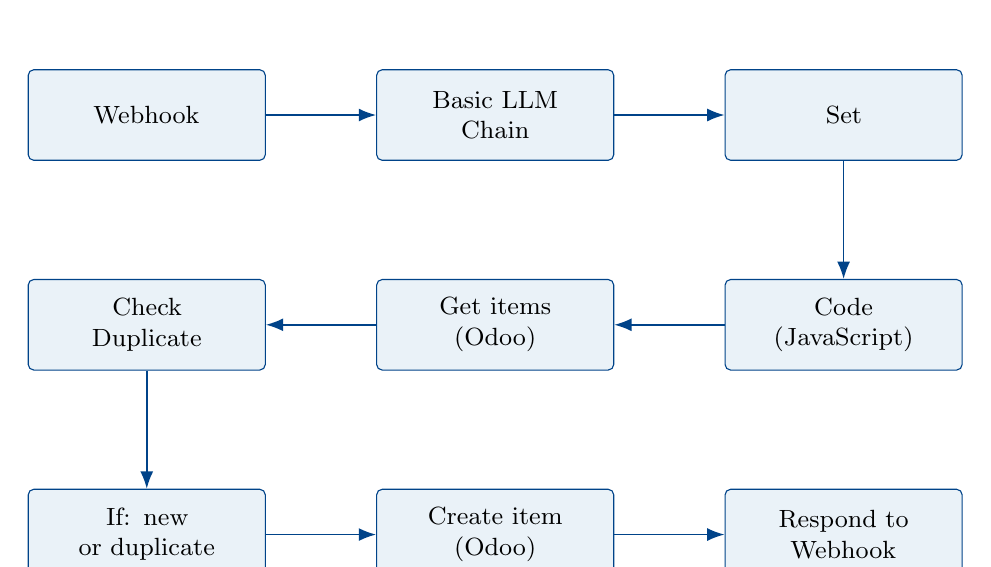
\begin{tikzpicture}[node distance=1.5cm and 1.4cm, >={Latex[length=2.6mm]},
   wf/.style={draw=IITBlue, fill=SoftBlue, rounded corners=2pt, align=center,
              font=\small, minimum height=1.15cm, text width=2.8cm, inner sep=3pt}]
% Row 1 (left to right)
\node[wf] (n1) {Webhook};
\node[wf, right=of n1] (n2) {Basic LLM\\Chain};
\node[wf, right=of n2] (n3) {Set};
% Row 2 (right to left)
\node[wf, below=of n3] (n4) {Code\\(JavaScript)};
\node[wf, left=of n4] (n5) {Get items\\(Odoo)};
\node[wf, left=of n5] (n6) {Check\\Duplicate};
% Row 3 (left to right)
\node[wf, below=of n6] (n7) {If: new\\or duplicate};
\node[wf, right=of n7] (n8) {Create item\\(Odoo)};
\node[wf, right=of n8] (n9) {Respond to\\Webhook};
% flow arrows (serpentine)
\draw[wfarr] (n1)--(n2);
\draw[wfarr] (n2)--(n3);
\draw[wfarr] (n3)--(n4);
\draw[wfarr] (n4)--(n5);
\draw[wfarr] (n5)--(n6);
\draw[wfarr] (n6)--(n7);
\draw[wfarr] (n7)--(n8);
\draw[wfarr] (n8)--(n9);
\end{tikzpicture}
\caption{Lead Capture workflow}
\label{fig:lead-capture-workflow}
\end{figure}
\figdesc{The workflow receives a customer message, extracts structured fields, checks Odoo for duplicates, and returns either a duplicate result or a newly created opportunity.}


The main nodes used in this workflow are:

\begin{itemize}
\item \textbf{Webhook:} receives the request sent by the web platform.
\item \textbf{Basic LLM Chain:} extracts useful information from the customer message.
\item \textbf{Ollama Chat Model:} provides the AI model used for text extraction.
\item \textbf{Set:} prepares the extracted fields in a cleaner format.
\item \textbf{Code in JavaScript:} applies simple rules and prepares the data.
\item \textbf{Get many items:} reads existing CRM opportunities from Odoo.
\item \textbf{Check Duplicate:} compares the new lead with existing records.
\item \textbf{If:} chooses between creating a new opportunity or returning a duplicate result.
\item \textbf{Create an item:} creates the opportunity in Odoo when no duplicate is found.
\item \textbf{Respond to Webhook:} sends the final result back to the platform.
\end{itemize}

\subsubsection{CRM Analytics Summary Workflow}

The CRM Analytics Summary workflow is used to give the manager a clearer view of the sales pipeline. It reads CRM records, calculates indicators, and prepares a readable summary.

The figure below shows this workflow as built in n8n.

\begin{figure}[H]
\centering
\resizebox{\textwidth}{!}{%
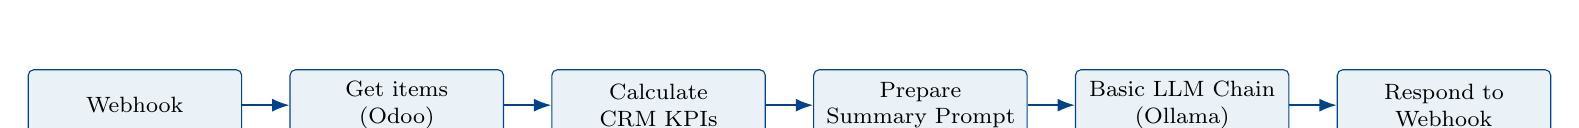
\begin{tikzpicture}[start chain=going right, node distance=6mm, >={Latex[length=2.2mm]}, every join/.style={wfarr}]
\node[wfnode, on chain] {Webhook};
\node[wfnode, on chain, join] {Get items\\(Odoo)};
\node[wfnode, on chain, join] {Calculate\\CRM KPIs};
\node[wfnode, on chain, join] {Prepare\\Summary Prompt};
\node[wfnode, on chain, join] {Basic LLM Chain\\(Ollama)};
\node[wfnode, on chain, join] {Respond to\\Webhook};
\end{tikzpicture}%
}
\caption{CRM Analytics Summary workflow}
\label{fig:crm analytics workflow}
\end{figure}
\figdesc{The workflow reads CRM opportunities, calculates reliable indicators, and converts the completed metrics into a concise management summary.}

The main nodes used in this workflow are:

\begin{itemize}
\item \textbf{Webhook:} starts the workflow when the platform requests a summary.
\item \textbf{Get many items:} retrieves CRM opportunities from Odoo.
\item \textbf{Calculate CRM KPIs:} calculates useful indicators from CRM data.
\item \textbf{Prepare Summary Prompt:} prepares the text sent to the AI model.
\item \textbf{Basic LLM Chain:} generates a readable CRM summary.
\item \textbf{Ollama Model:} provides the AI model used for summarization.
\item \textbf{Respond to Webhook:} returns the summary to the web platform.
\end{itemize}

\subsubsection{Smart Follow-Up Workflow}

The Smart Follow-Up workflow helps the user detect leads that have not been updated for a period of time. It also prepares a follow-up message that can be used to contact the customer again.

The figure below shows this workflow as built in n8n.

\begin{figure}[H]
\centering
\resizebox{\textwidth}{!}{%
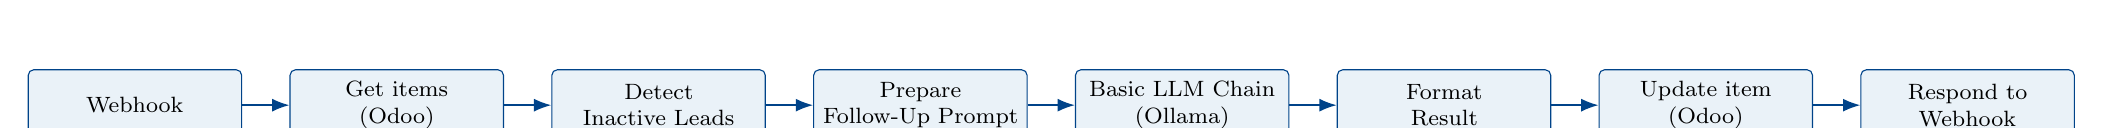
\begin{tikzpicture}[start chain=going right, node distance=6mm, >={Latex[length=2.2mm]}, every join/.style={wfarr}]
\node[wfnode, on chain] {Webhook};
\node[wfnode, on chain, join] {Get items\\(Odoo)};
\node[wfnode, on chain, join] {Detect\\Inactive Leads};
\node[wfnode, on chain, join] {Prepare\\Follow-Up Prompt};
\node[wfnode, on chain, join] {Basic LLM Chain\\(Ollama)};
\node[wfnode, on chain, join] {Format\\Result};
\node[wfnode, on chain, join] {Update item\\(Odoo)};
\node[wfnode, on chain, join] {Respond to\\Webhook};
\end{tikzpicture}%
}
\caption{Smart Follow-Up workflow}
\label{fig:smart followup workflow}
\end{figure}
\figdesc{The workflow finds inactive opportunities, prepares a follow-up draft for each one, and returns the reviewable results to the platform.}


The main nodes used in this workflow are:

\begin{itemize}
\item \textbf{Webhook:} receives the follow-up request from the platform.
\item \textbf{Get many items:} reads the CRM opportunities.
\item \textbf{Detect Inactive Leads:} identifies leads that need attention.
\item \textbf{Prepare Follow-Up Prompt:} prepares the information for the AI model.
\item \textbf{Basic LLM Chain:} generates a follow-up message.
\item \textbf{Ollama Model:} provides the AI model used to write the message.
\item \textbf{Format Follow-Up Result:} organizes the final response.
\item \textbf{Update an item:} updates the CRM record when needed.
\item \textbf{Respond to Webhook:} sends the result back to the platform.
\end{itemize}

\subsubsection{AI Assistant Workflow}

The AI Assistant workflow allows the user to ask CRM-related questions in natural language. It connects the assistant to CRM tools so that the user can search, create, or update opportunities more easily.

The figure below shows this workflow as built in n8n.

\begin{figure}[H]
\centering
\resizebox{\textwidth}{!}{%
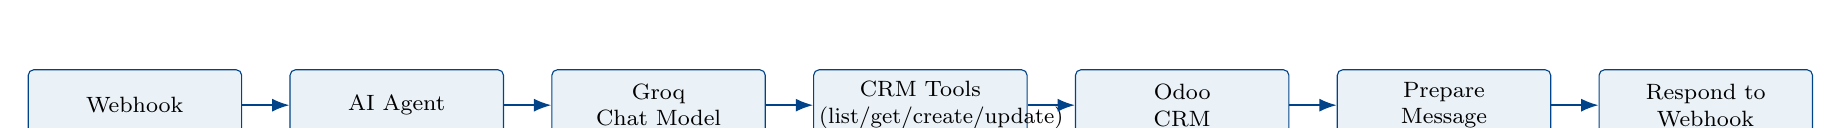
\begin{tikzpicture}[start chain=going right, node distance=6mm, >={Latex[length=2.2mm]}, every join/.style={wfarr}]
\node[wfnode, on chain] {Webhook};
\node[wfnode, on chain, join] {AI Agent};
\node[wfnode, on chain, join] {Groq\\Chat Model};
\node[wfnode, on chain, join] {CRM Tools\\(list/get/create/update)};
\node[wfnode, on chain, join] {Odoo\\CRM};
\node[wfnode, on chain, join] {Prepare\\Message};
\node[wfnode, on chain, join] {Respond to\\Webhook};
\end{tikzpicture}%
}
\caption{AI Assistant workflow}
\label{fig:ai assistant workflow}
\end{figure}
\figdesc{The workflow sends the user's question to a controlled agent, lets the agent select approved CRM tools, and returns a clean answer to the interface.}


The main nodes used in this workflow are:

\begin{itemize}
\item \textbf{Webhook:} receives the user question from the web platform.
\item \textbf{AI Agent:} understands the question and decides which CRM action is needed.
\item \textbf{Groq Chat Model:} provides the AI model used by the assistant.
\item \textbf{List Opportunities:} retrieves CRM opportunities.
\item \textbf{Create Opportunity:} creates a new CRM opportunity when requested.
\item \textbf{Get Opportunity:} retrieves the details of a specific opportunity.
\item \textbf{Get CRM Notes:} reads notes related to CRM records.
\item \textbf{Update Opportunity Phone:} updates the phone number of an opportunity.
\item \textbf{Update Opportunity Name:} updates the customer name.
\item \textbf{Update Opportunity Email:} updates the customer email address.
\item \textbf{Prepare Website Message:} prepares a clean answer for the user interface.
\item \textbf{Respond to Webhook:} sends the assistant response back to the platform.
\end{itemize}

\subsubsection{CRM List Leads Workflow}

The CRM List Leads workflow is used to display CRM opportunities inside the platform. It gives the user a simple way to view CRM records without navigating directly inside Odoo.

The figure below shows this workflow as built in n8n.

\begin{figure}[H]
\centering
\resizebox{\textwidth}{!}{%
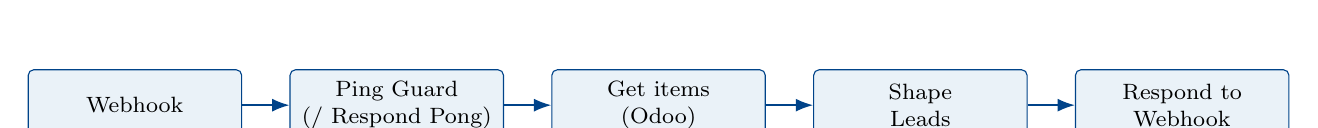
\begin{tikzpicture}[start chain=going right, node distance=6mm, >={Latex[length=2.2mm]}, every join/.style={wfarr}]
\node[wfnode, on chain] {Webhook};
\node[wfnode, on chain, join] {Ping Guard\\(/ Respond Pong)};
\node[wfnode, on chain, join] {Get items\\(Odoo)};
\node[wfnode, on chain, join] {Shape\\Leads};
\node[wfnode, on chain, join] {Respond to\\Webhook};
\end{tikzpicture}%
}
\caption{CRM List Leads workflow}
\label{fig:crm list leads workflow}
\end{figure}
\figdesc{The workflow performs a read-only retrieval of CRM opportunities, reshapes the records, and returns a consistent list for the workspace.}


The main nodes used in this workflow are:

\begin{itemize}
\item \textbf{Webhook:} receives the request to list CRM leads.
\item \textbf{Ping Guard:} checks if the request is only a connection test.
\item \textbf{Respond Pong:} confirms that the workflow is active.
\item \textbf{Get many items:} reads the CRM opportunities from Odoo.
\item \textbf{Shape Leads:} formats the records before sending them to the platform.
\item \textbf{Respond to Webhook:} returns the list of leads to the web platform.
\end{itemize}

\subsection{Conceptual Design}\label{sumlbl:c2s2ss2}

The conceptual design presents the platform from a functional point of view before moving to the implementation sprints. It helps explain what the user can do inside the system and how the main features are connected. In this part, the focus is placed on the global use case diagram. The sequence diagrams are presented later inside each sprint, because each sprint contains a specific workflow with its own execution logic.

\subsubsection{Global Use Case Diagram}

The global use case diagram presents the main actions that can be performed by the user inside the platform. The main actor is the platform user, who can sign in, capture a lead, check duplicates, create opportunities, view CRM indicators, generate follow-up messages, ask the CRM assistant, and manage the live CRM connection.


The main use cases of the platform are:

\begin{itemize}
\item \textbf{Sign in:} allows the user to access the platform securely.
\item \textbf{Capture lead:} allows the user to transform a customer message into CRM data.
\item \textbf{Check duplicate:} verifies if the customer already exists in the CRM.
\item \textbf{Create opportunity:} creates a new opportunity when no duplicate is found.
\item \textbf{View dashboard:} displays CRM indicators and sales information.
\item \textbf{Generate follow-up:} helps the user contact inactive leads.
\item \textbf{Ask CRM assistant:} allows the user to ask CRM questions in natural language.
\item \textbf{Manage live connection:} allows the platform to communicate with n8n workflows and Odoo CRM.
\end{itemize}

\begin{figure}[H]
\centering
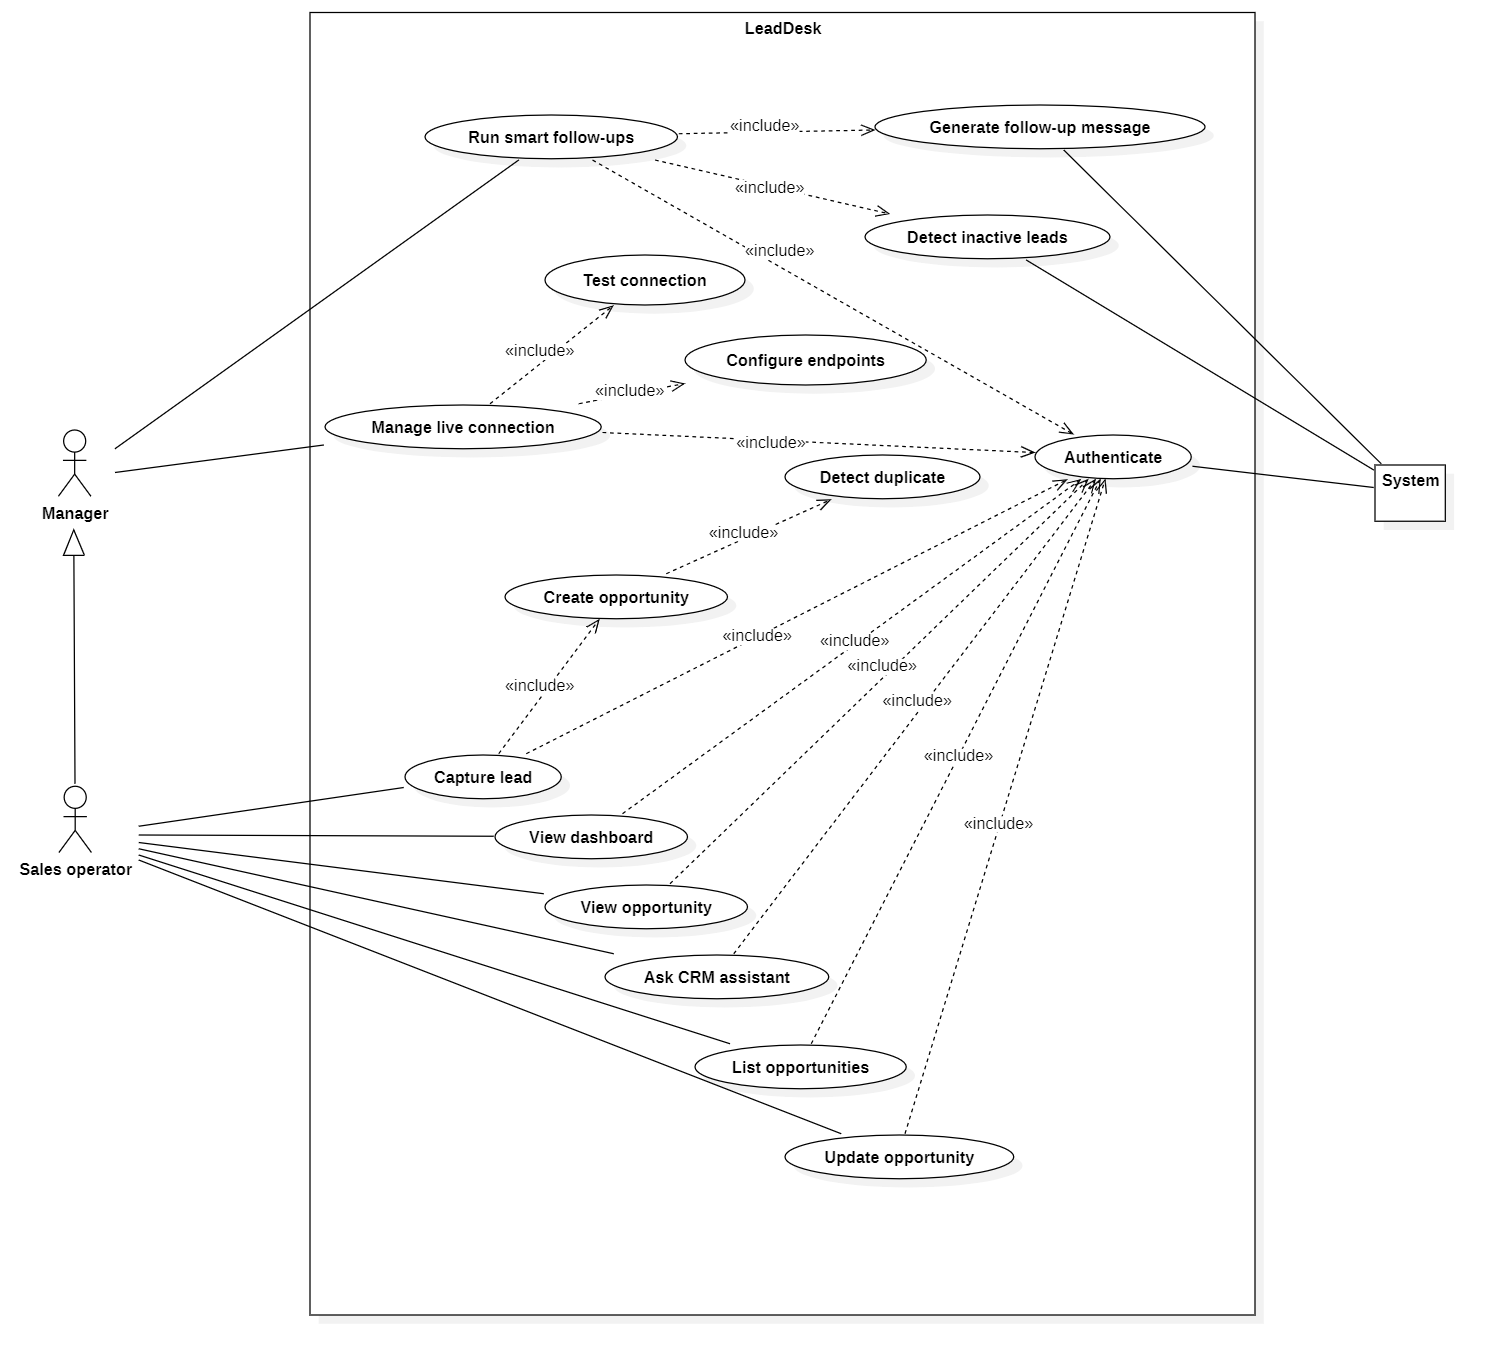
\includegraphics[width=\textwidth,height=0.9\textheight,keepaspectratio]{umls/img/uc-global.png}
\caption{Global use case diagram of LeadDesk}
\label{fig:uc-global}
\end{figure}
\figdesc{The diagram consolidates the principal actions available across the platform and the automated services that support them.}

\noindent\textbf{Actor responsibilities.}
\begin{itemize}
\item \textbf{Manager:} supervises CRM activity by viewing the dashboard and opportunities, running follow-ups, using the assistant, updating records, and managing the live connection.
\item \textbf{Sales operator:} performs daily sales work by creating an account, signing in, capturing leads, consulting and updating opportunities, viewing the dashboard, and asking the assistant for CRM information.
\item \textbf{System:} represents the backend automation composed of the server, n8n workflows, Odoo CRM, and language models; it authenticates requests, processes CRM data, detects duplicates and inactivity, and executes approved operations.
\end{itemize}


% ===== Sequence-diagram helper macros =====
\newcommand{\lifeline}[2]{\draw[lifeline] (#1.south) -- (#1 |- 0,#2);}
\newcommand{\msgR}[4]{\draw[smsg] (#1 |- 0,#3) -- (#2 |- 0,#3) node[midway,above,font=\scriptsize,text=black]{#4};}
\newcommand{\msgL}[4]{\draw[rmsg] (#1 |- 0,#3) -- (#2 |- 0,#3) node[midway,above,font=\scriptsize,text=black]{#4};}
\newcommand{\selfstep}[3]{\node[snote] at (#1 |- 0,#2) {#3};}

\chapter{Business Workflows of the Platform}

\vspace{0.35cm}
{\Large\bfseries Summary}\par
\vspace{3pt}{\color{black}\hrule height 0.6pt}\vspace{0.30cm}
{\small
\chsummaryitem{3.1}{Introduction}{sumlbl:c3s1}
\chsummaryitem{3.2}{Lead Capture Workflow}{sumlbl:c3s2}
\chsummaryitem{3.3}{CRM Analytics Summary Workflow}{sumlbl:c3s3}
\chsummaryitem{3.4}{Smart Follow-Up Workflow}{sumlbl:c3s4}
\chsummaryitem{3.5}{AI Assistant Workflow}{sumlbl:c3s5}
\chsummaryitem{3.6}{CRM List Leads Workflow}{sumlbl:c3s6}
\chsummaryitem{3.7}{Internal Chat Workflow}{sumlbl:c3s7}
\chsummaryitem{3.8}{Workflow Overview}{sumlbl:c3s8}
\chsummaryitem{3.9}{Conclusion}{sumlbl:c3s9}
}
\clearpage

\section{Introduction}\label{sumlbl:c3s1}
This chapter presents the workflows that carry the business logic of the platform. Each workflow turns a user action into a concrete CRM result, such as capturing a lead, computing a summary, drafting a follow-up message, or answering a question. The goal here is to explain what each workflow does and when it runs, in clear terms. The detailed step-by-step exchanges are shown later as sequence diagrams inside the sprint chapters, where each feature is built.

The platform uses six workflows. Five of them are reached through a webhook and are used by the web console. The sixth one is a chat-based version of the assistant that was used during development.

\section{Lead Capture Workflow}\label{sumlbl:c3s2}
The lead capture workflow is the entry point for new customers. It receives a free-text message written by a sales operator, asks the language model to read the message and return clean fields, and then checks whether the customer already exists. The fields are the name, the email, the phone, the interest, the intent, and a priority. A short piece of logic compares the new email and phone with the opportunities already stored in Odoo. When the customer is new, the workflow creates the opportunity. When the customer already exists, it returns a duplicate result instead of creating a second record. The model is used only to read the message; the duplicate decision is made by code so that the result stays predictable.

\section{CRM Analytics Summary Workflow}\label{sumlbl:c3s3}
The analytics workflow gives the manager a quick view of the pipeline. It reads the opportunities from Odoo and computes five indicators: the total number of opportunities, the opportunities that have an email, the opportunities that have a phone, the inactive opportunities, and the opportunities created during the current week. The numbers are calculated by code first. Only after that, the model receives the finished numbers and writes a short readable summary. The prompt forbids the model from inventing values, so the summary always matches the real data.

\section{Smart Follow-Up Workflow}\label{sumlbl:c3s4}
The follow-up workflow helps the team contact leads that went quiet. It reads the opportunities, keeps the ones whose last update is at least seven days old, and keeps a single record per email so the same person is not contacted twice. For each selected lead, the model drafts a short professional message that uses the lead name, recalls the previous interest, and asks whether the customer wants to continue. The drafted message is then saved back to the description of the opportunity in Odoo.

\section{AI Assistant Workflow}\label{sumlbl:c3s5}
The assistant workflow lets a user talk to the CRM in natural language. It is built around an agent that can call a small set of controlled tools: list opportunities, read one opportunity, create an opportunity, read CRM notes, and update a name, a phone, or an email. The agent does not have free access to the system. It can only use the tools it was given, and its answers follow strict formatting rules so the reply is clean and easy to read in the interface. This makes the assistant useful and safe to explain.

\section{CRM List Leads Workflow}\label{sumlbl:c3s6}
This read-only workflow feeds the workspace page. It reads the opportunities from Odoo, keeps the records that are real opportunities, fills empty fields with safe defaults, maps the priority values, cleans the descriptions, and returns a list in the exact shape the interface expects. Because it only reads data, it is a safe workflow to call often.

\section{Internal Chat Workflow}\label{sumlbl:c3s7}
The internal chat workflow is a chat-trigger version of the assistant. It is not the main endpoint used by the console, but it helped shape the idea of a CRM agent connected to Odoo tools. It stays in the project as a development and experimentation workflow.

\section{Workflow Overview}\label{sumlbl:c3s8}
The table below summarizes the six workflows, what each one does, and when it runs.

\begin{table}[H]
\centering
\small
\begin{tabularx}{\textwidth}{|p{3.4cm}|X|p{4.1cm}|}
\hline\rowcolor{TabHead}
\textbf{Workflow} & \textbf{What it does} & \textbf{Runs when} \\
\hline
Lead Capture & Reads a customer message and creates a new opportunity while avoiding duplicates & A new lead message is submitted \\
\hline
CRM Analytics Summary & Computes the pipeline indicators and writes a short summary & The dashboard is opened \\
\hline
Smart Follow-Up & Finds inactive leads and drafts a polite follow-up message & The follow-up center is opened \\
\hline
AI Assistant & Answers CRM questions and performs controlled actions through tools & The user asks the assistant \\
\hline
CRM List Leads & Returns a clean list of opportunities for the workspace & The workspace loads live data \\
\hline
Internal Chat & A chat-based assistant used during development & Used for internal testing \\
\hline
\end{tabularx}
\caption{Overview of the platform workflows}
\end{table}

\section{Conclusion}\label{sumlbl:c3s9}
This chapter described the role of each workflow in plain terms. Lead capture creates clean opportunities, the analytics workflow reports trustworthy numbers, the follow-up workflow reactivates quiet leads, and the assistant gives a conversational way to work with CRM data. The next chapter presents the system architecture and the technologies that hold these workflows together.


\chapter{System Architecture and Technologies}

\vspace{0.35cm}
{\Large\bfseries Summary}\par
\vspace{3pt}{\color{black}\hrule height 0.6pt}\vspace{0.30cm}
{\small
\chsummaryitem{4.1}{Introduction}{sumlbl:c4s1}
\chsummaryitem{4.2}{Development Environment}{sumlbl:c4s2}
\chsummaryitem{4.3}{Front-End Technologies}{sumlbl:c4s3}
\chsummaryitem{4.4}{Backend Technologies}{sumlbl:c4s4}
\chsummaryitem{4.5}{Database and Persistence}{sumlbl:c4s5}
\chsummaryitem{4.6}{Automation and CRM Tools}{sumlbl:c4s6}
\chsummaryitem{4.7}{AI Models}{sumlbl:c4s7}
\chsummaryitem{4.8}{Global Architecture}{sumlbl:c4s8}
\chsummaryitem{4.9}{Conclusion}{sumlbl:c4s9}
}
\clearpage

\section{Introduction}\label{sumlbl:c4s1}
This chapter presents the technologies and the architecture used to build LeadDesk. The stack was chosen to stay clear for a student project while remaining realistic for a business application. The platform combines simple web technologies, a structured backend, and a workflow automation layer, so each part has one clear job.

\section{Development Environment}\label{sumlbl:c4s2}
The development environment was kept light. The application runs locally with Node.js, and the automation layer connects to n8n and Odoo when real CRM tests are needed. This setup made it possible to build the platform step by step and to test each feature on a normal laptop.

The table below lists the main tools and technologies of the development environment.

\begin{table}[H]
\centering
\begin{tabularx}{\textwidth}{|p{4cm}|X|}
\hline\rowcolor{TabHead}
\textbf{Category} & \textbf{Tools and technologies} \\
\hline
Code editor & Visual Studio Code or another modern editor \\
\hline
Runtime & Node.js with an Express backend \\
\hline
Front-end & HTML, CSS, JavaScript, and SVG charts \\
\hline
Local database & NeDB files stored on the server \\
\hline
Automation & n8n workflows \\
\hline
CRM & Odoo CRM, on the crm.lead model \\
\hline
AI & Ollama local models and a Groq model for the assistant \\
\hline
\end{tabularx}
\caption{Software environment used during development}
\end{table}

\section{Front-End Technologies}\label{sumlbl:c4s3}
The front end is a web console built with HTML, CSS, and plain JavaScript. This choice was on purpose. Instead of a heavy framework, the project uses a clear structure based on the Model, View, and Controller idea. The Model holds the data and the calls to the backend. The View holds the rendering, the charts, and the formatting. The Controller handles navigation, events, and the link between the View and the Model.

The interface was designed for a sales team. It has a sidebar, a dashboard, a lead capture form, a lead workspace, a follow-up center, a CRM assistant, an architecture page, and a settings page. The navigation is grouped into Operations, Intelligence, and System sections, so the user always knows where each feature belongs.

The figure below shows the front-end organization based on the Model-View-Controller idea.

\begin{figure}[H]
\centering
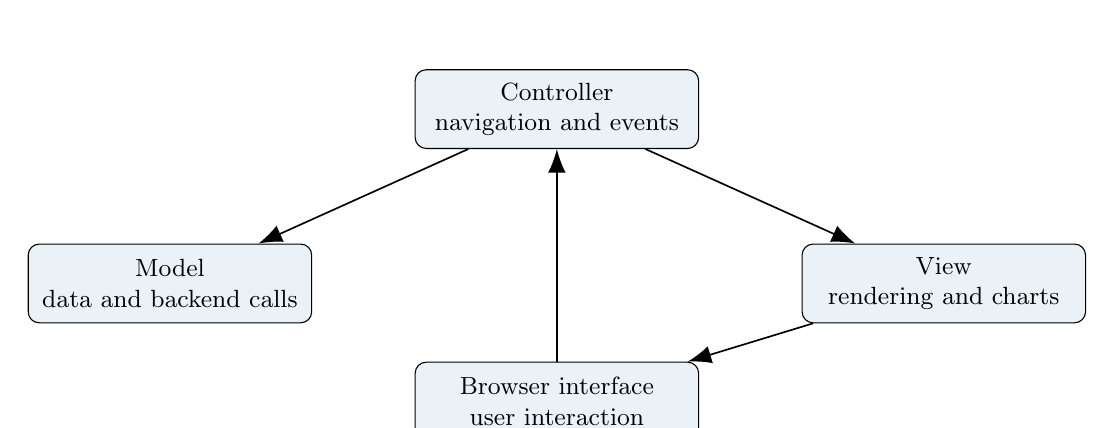
\begin{tikzpicture}[node distance=1.3cm, every node/.style={font=\small}]
\tikzset{box/.style={draw, rounded corners, fill=SoftBlue, minimum width=3.6cm, minimum height=1cm, align=center}}
\tikzset{arrow/.style={-{Latex[length=3mm]}, semithick}}
\node[box] (controller) {Controller\\navigation and events};
\node[box, below left=1.2cm and 1.3cm of controller] (model) {Model\\data and backend calls};
\node[box, below right=1.2cm and 1.3cm of controller] (view) {View\\rendering and charts};
\node[box, below=2.7cm of controller] (browser) {Browser interface\\user interaction};
\draw[arrow] (controller) -- (model);
\draw[arrow] (controller) -- (view);
\draw[arrow] (view) -- (browser);
\draw[arrow] (browser) -- (controller);
\end{tikzpicture}
\caption{Front-end organization based on a simple Model-View-Controller separation}
\end{figure}
\figdesc{The diagram separates stored state and API access in the model, interface rendering in the view, and user-action coordination in the controller.}

\section{Backend Technologies}\label{sumlbl:c4s4}
The backend is built with Node.js and Express. It serves the web application, exposes the API, handles authentication, stores the local data, computes local summaries, runs the local assistant behaviour, and forwards live requests to n8n. The backend keeps three clear layers. The routes receive the requests and check the input. The services hold the business logic. The repositories are the only part that reads and writes the local database. This separation avoids mixing the web code, the logic, and the data access in the same place, and it makes the project easier to explain.

The table below describes the three backend layers and their responsibilities.

\begin{table}[H]
\centering
\begin{tabularx}{\textwidth}{|p{3.6cm}|X|}
\hline\rowcolor{TabHead}
\textbf{Layer} & \textbf{Responsibility} \\
\hline
Routes & Receive the API calls, check the input, and call the right service \\
\hline
Services & Hold the logic for authentication, lead capture, analytics, the assistant, and live calls \\
\hline
Repositories & The only layer that reads and writes the local database \\
\hline
\end{tabularx}
\caption{Backend layers and their responsibilities}
\end{table}

\section{Database and Persistence}\label{sumlbl:c4s5}
For the local version, the platform uses NeDB, a small embedded database that stores its collections as files. This fits the project because the application must be simple to run. The local database holds the users, the opportunities, the captures, and the settings. On the first start, the backend creates an initial user and a starter set of opportunities so the interface is ready to use.

The CRM system of record for the live integration is Odoo. The workflows then work on the crm.lead model and treat the records marked as opportunities. The local database and Odoo are not meant to replace each other. The local store keeps the application easy to run, while Odoo provides the real CRM integration.

The local data model is presented below in three complementary views: a class diagram, an entity--association view, and a database view. All three share the same central \emph{Database} that stores the four collections (users, opportunities, captures, and settings).

\begin{figure}[H]
\centering
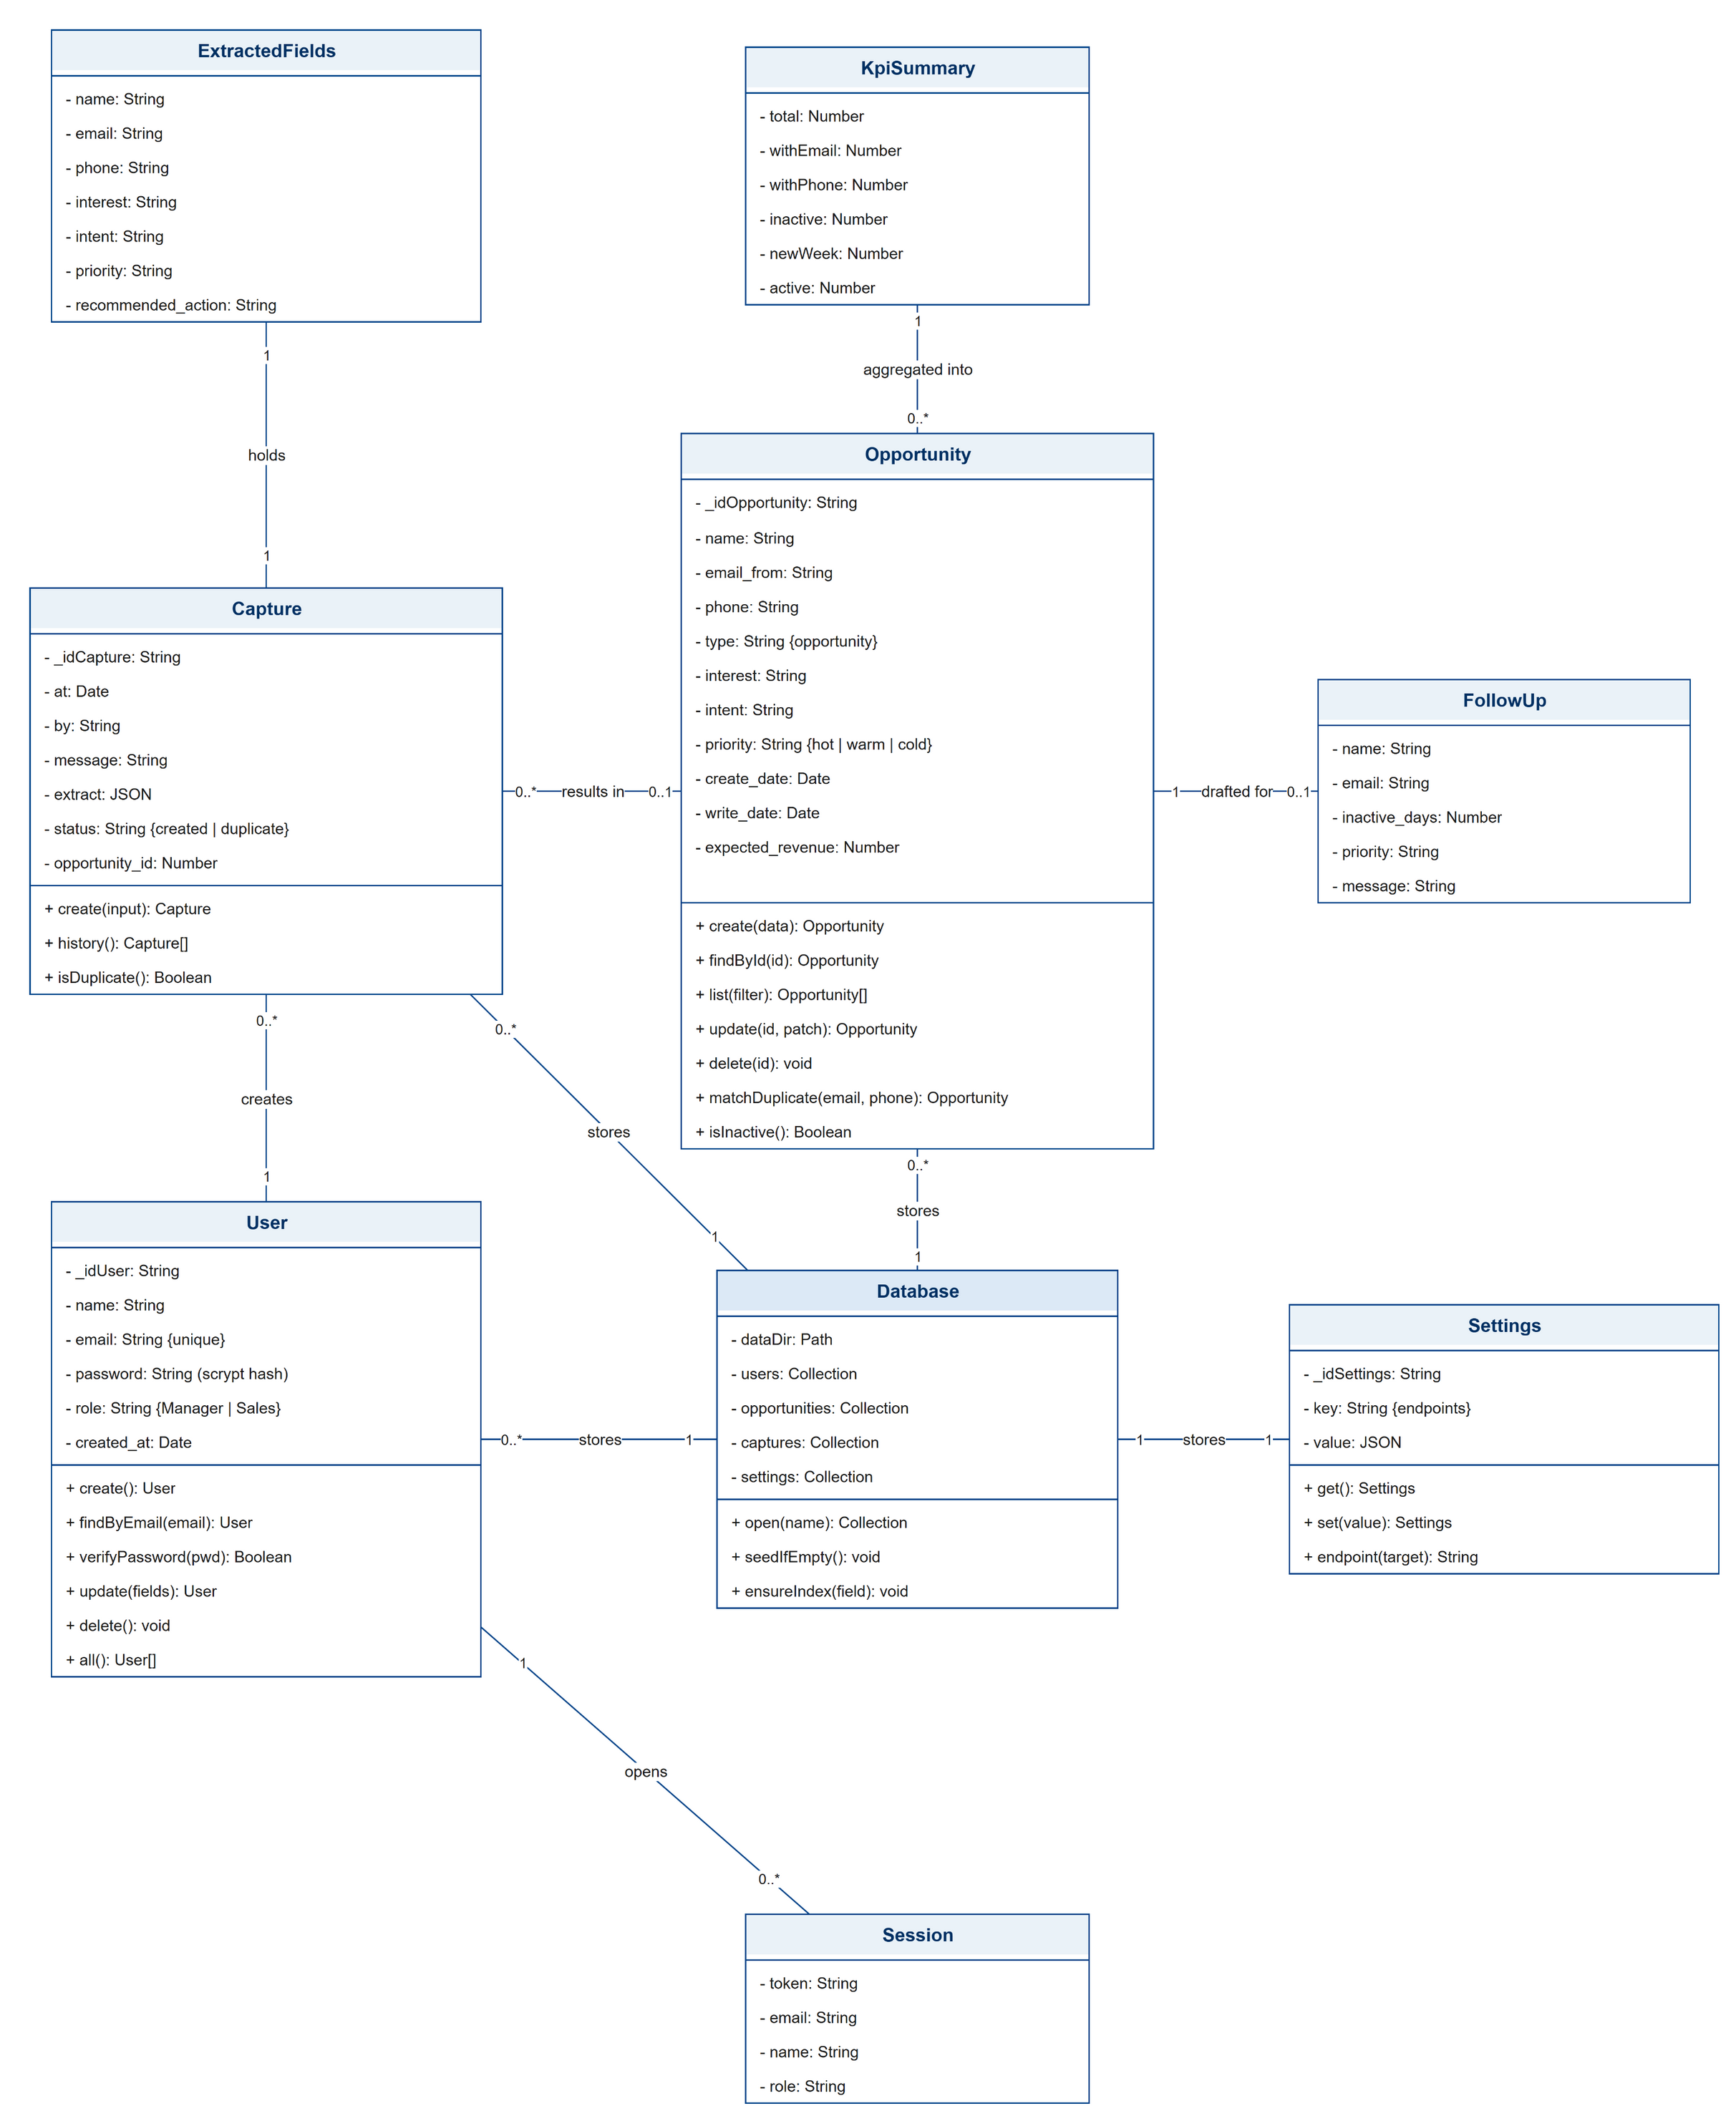
\includegraphics[width=\textwidth,height=0.85\textheight,keepaspectratio]{umls/img/class-domain.png}
\caption{Class diagram of the local data model used by NeDB}
\end{figure}
\figdesc{The class diagram presents the main local entities, their attributes, and the relationships used to persist accounts, sessions, opportunities, and capture records.}

The entity--association view highlights the entities and the associations between them together with their cardinalities.

\begin{figure}[H]
\centering
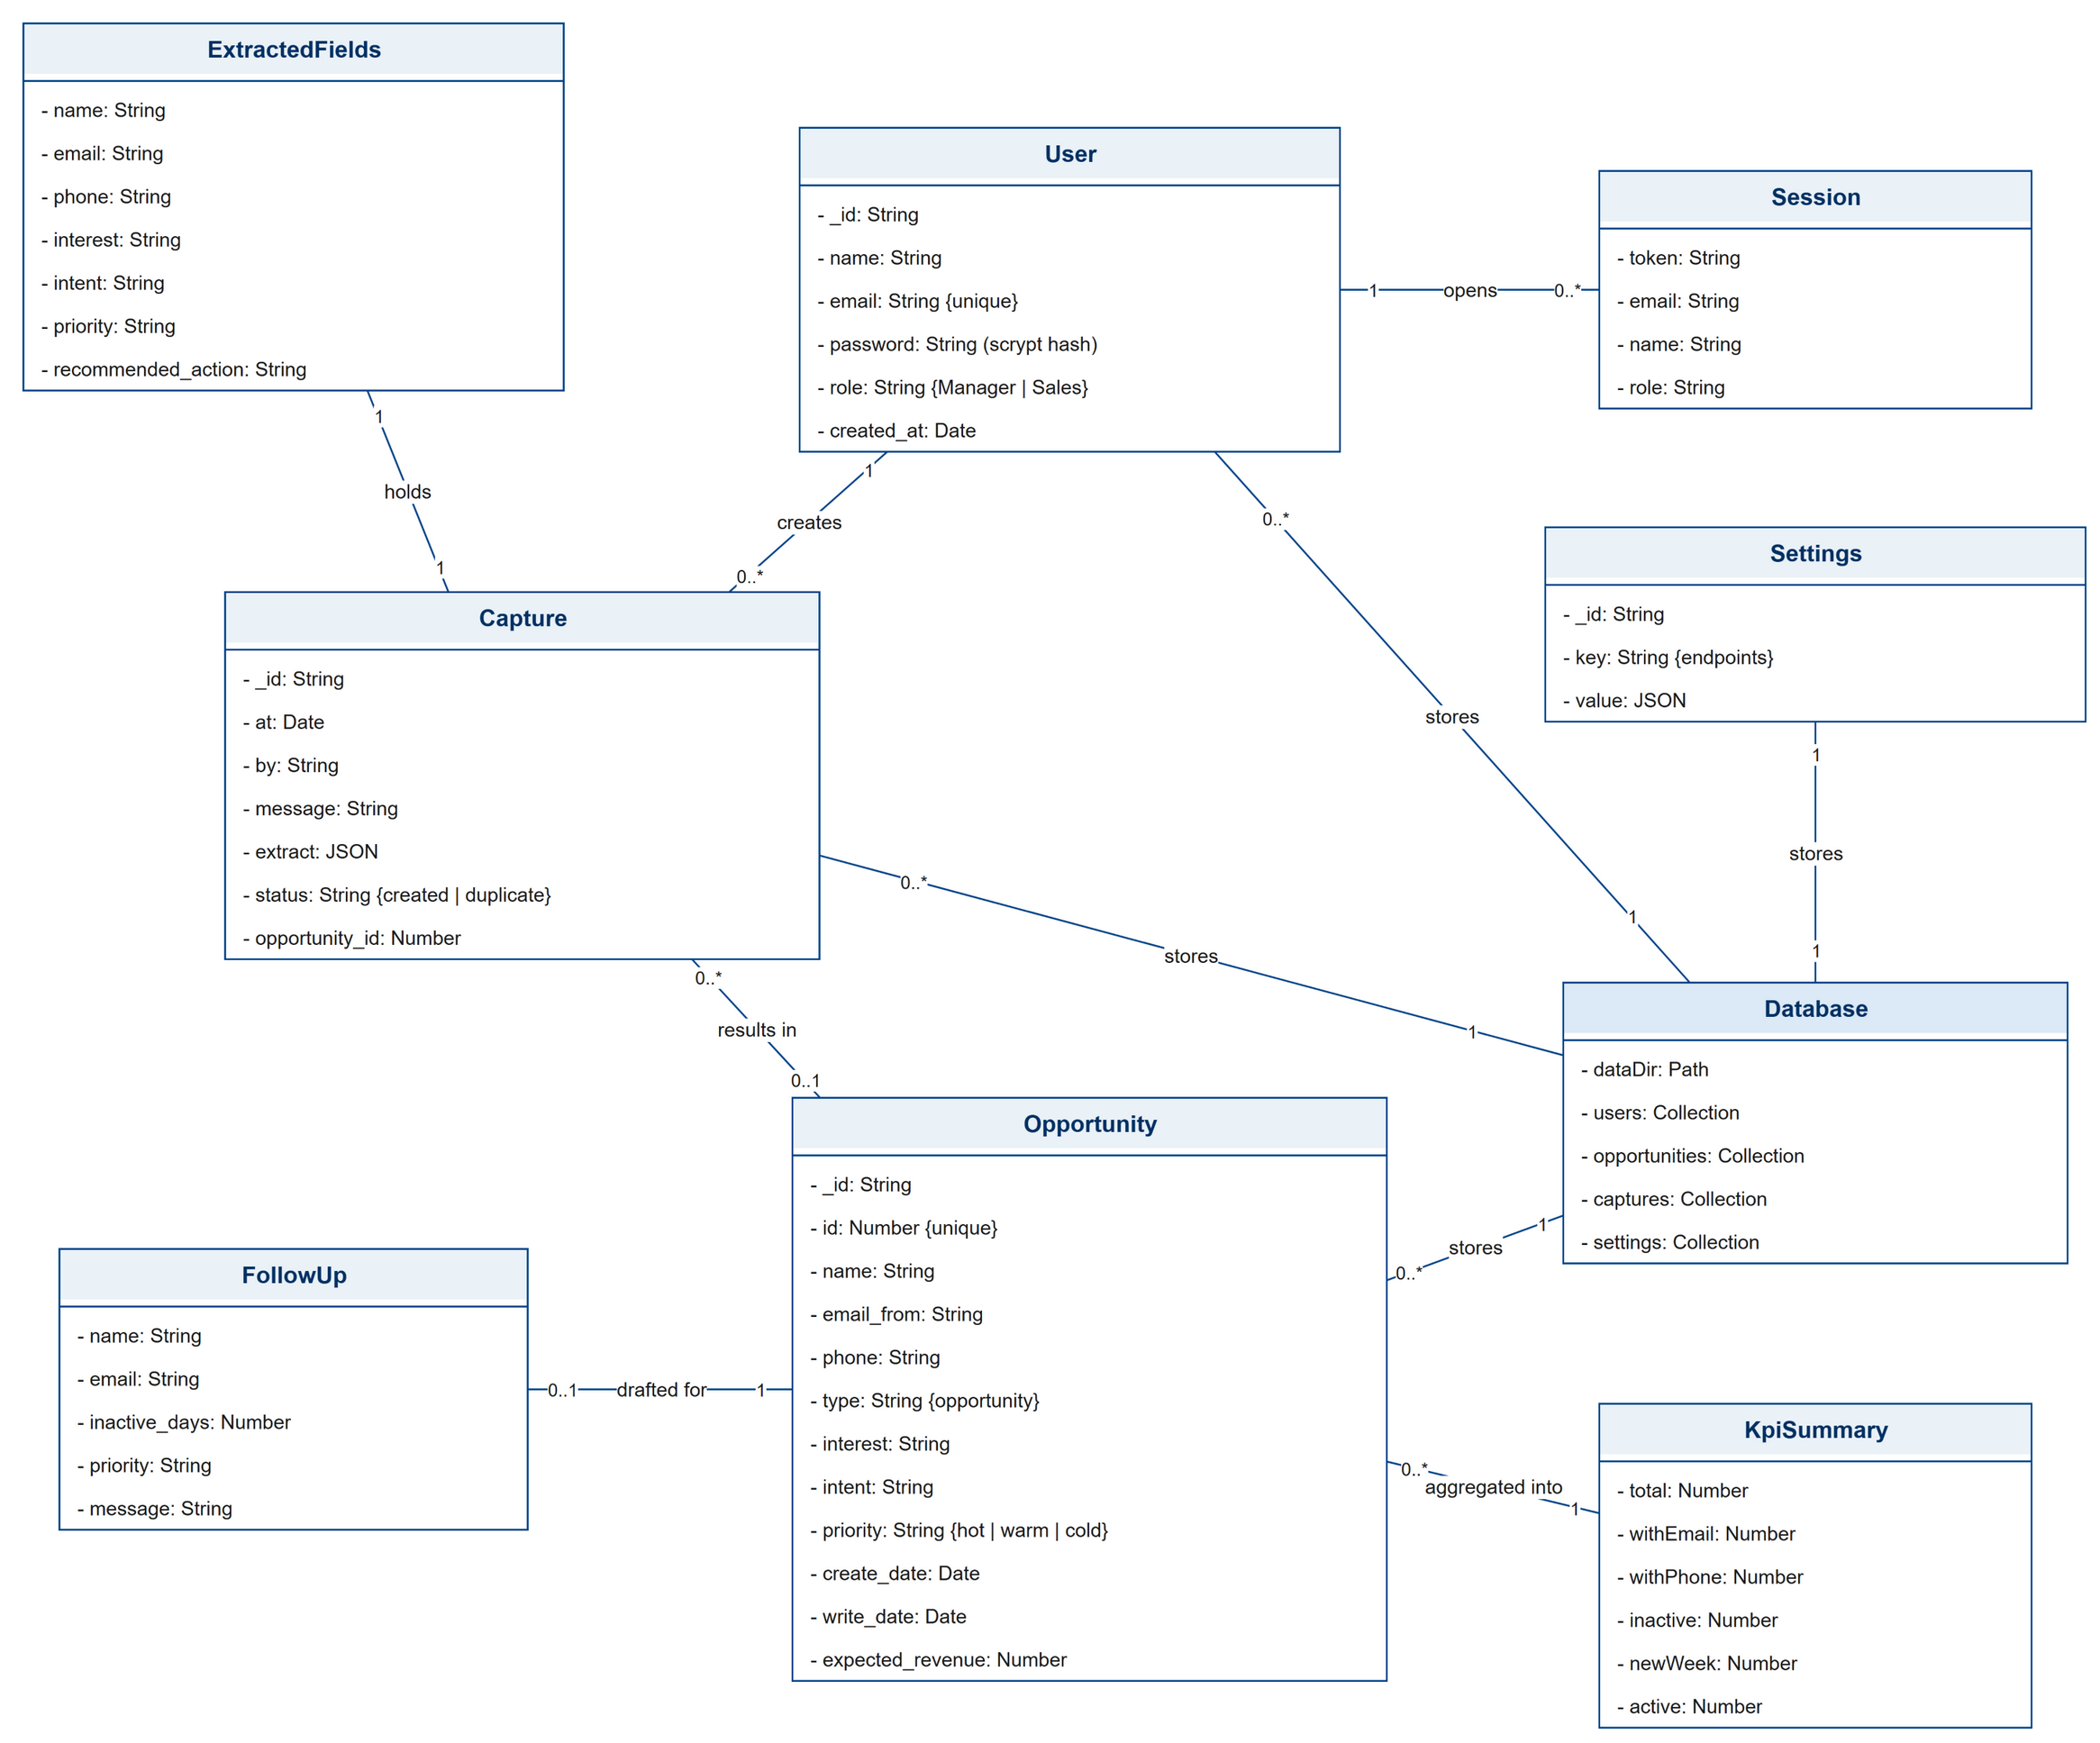
\includegraphics[width=\textwidth,height=0.85\textheight,keepaspectratio]{umls/img/entity-association.png}
\caption{Entity--association view of the local data model}
\end{figure}
\figdesc{The entity--association view emphasizes how the local entities connect and shows the cardinality of each relationship.}

The database view presents the four collections as they are physically stored, with their primary keys and the foreign-key references between them.

\begin{figure}[H]
\centering
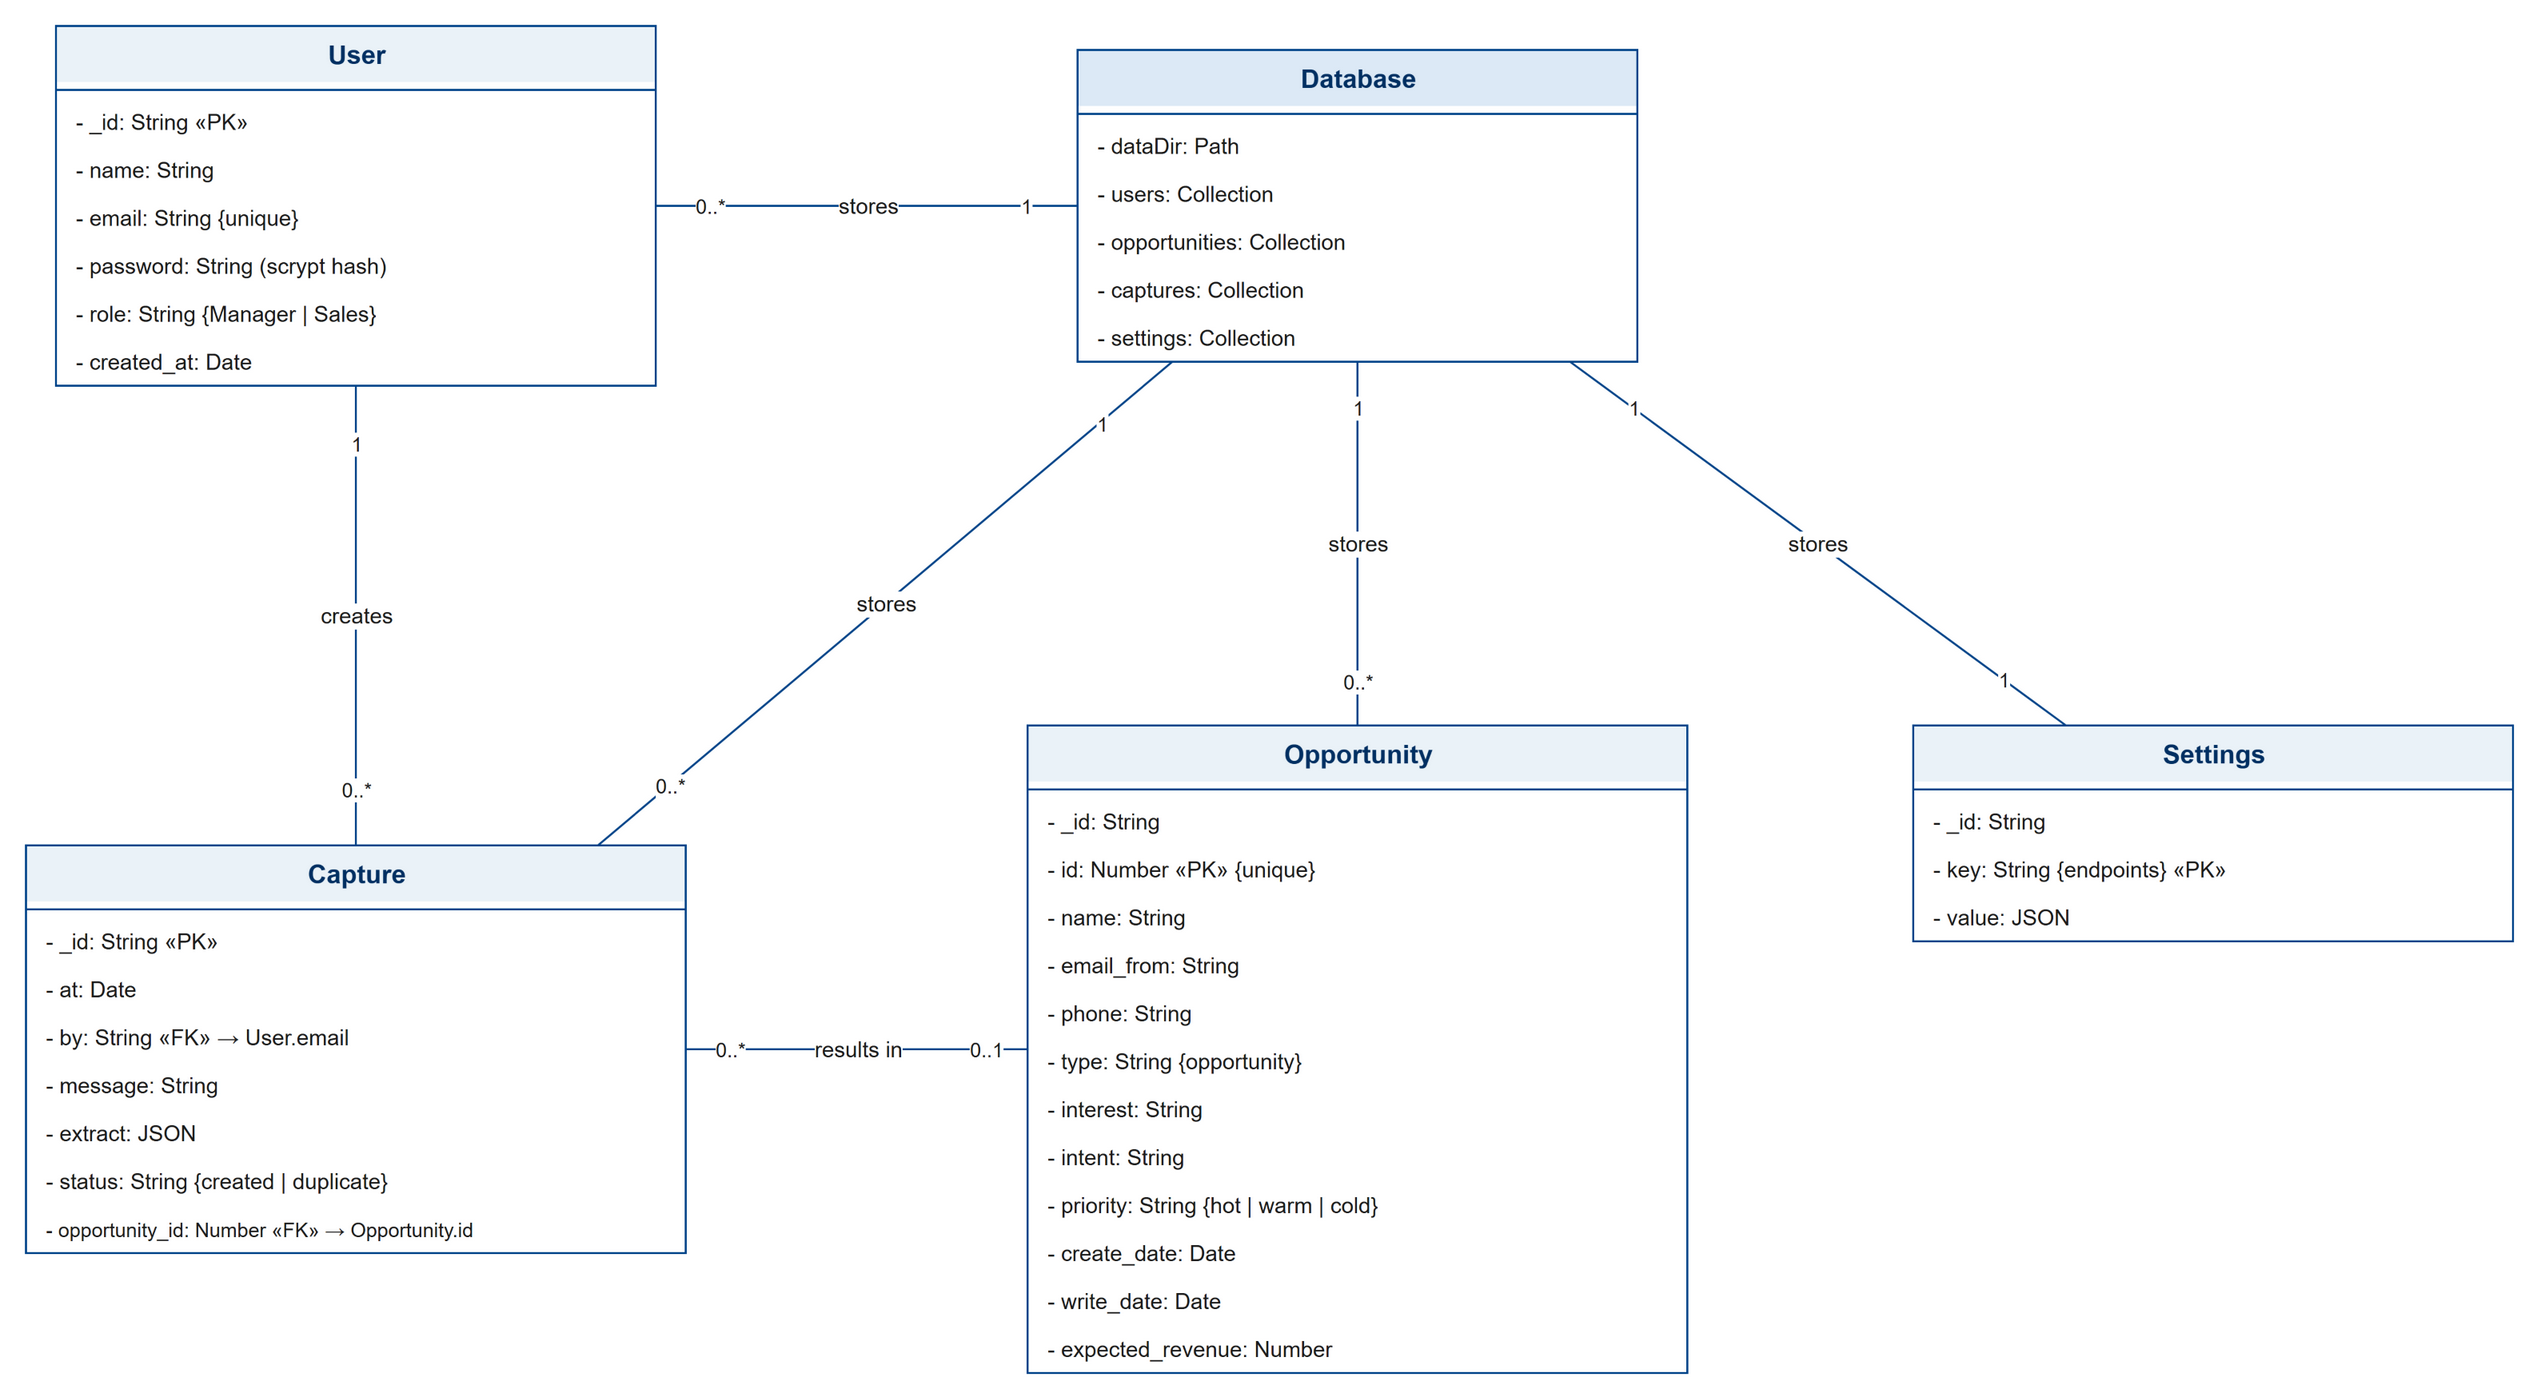
\includegraphics[width=\textwidth,height=0.85\textheight,keepaspectratio]{umls/img/database.png}
\caption{Database view of the local data model (collections, keys, and references)}
\end{figure}
\figdesc{The database view translates the conceptual model into NeDB collections and identifies the keys and references used to connect stored documents.}

\section{Automation and CRM Tools}\label{sumlbl:c4s6}
The automation layer is built with n8n. This tool was chosen because it gives a visual and readable way to connect webhooks, code steps, CRM actions, and AI steps. Each workflow can be opened and checked step by step, which helps during debugging and during the oral presentation. Odoo CRM holds the real records. The workflows act on crm.lead opportunities, so the project stays compatible with a standard CRM structure.

The table below lists the workflows and the webhook path used to reach each one.

\begin{table}[H]
\centering
\small
\begin{tabularx}{\textwidth}{|p{4cm}|X|p{3.3cm}|}
\hline\rowcolor{TabHead}
\textbf{Workflow} & \textbf{Purpose} & \textbf{Webhook path} \\
\hline
Lead Capture & Capture a lead and check duplicates & /lead-capture \\
\hline
CRM Analytics Summary & Compute KPIs and a summary & /crm-summary \\
\hline
Smart Follow-Up & Find inactive leads and draft messages & /smart-follow-up \\
\hline
AI Assistant & Conversational CRM actions & /crm-ai-assistant \\
\hline
CRM List Leads & Read opportunities for the workspace & /crm-list-leads \\
\hline
Internal Chat & Development assistant & chat trigger \\
\hline
\end{tabularx}
\caption{The platform workflows and how they are reached}
\end{table}

\section{AI Models}\label{sumlbl:c4s7}
AI is used only where it adds real value: reading fields from a customer message, writing a manager summary, drafting follow-up messages, and answering CRM questions through tools. The model is never allowed to decide business facts on its own. The workflows use a temperature of zero so the same input gives the same output, which is important for a CRM. When the assistant uses a larger model, it still works through defined tools and a strict system prompt.

\section{Global Architecture}\label{sumlbl:c4s8}
The architecture is split into a presentation layer, a backend layer, an automation layer, and a CRM layer, so each part has a clear job. The front end never reaches Odoo directly. It calls the backend. The backend either answers locally or forwards the request to n8n. n8n holds the workflow logic and talks to Odoo and to the model.

The live proxy is an important part of this design. When a browser calls n8n directly, it can hit CORS errors or long waits when the model is slow. The backend proxy solves this: the browser calls the backend on the same origin, and the backend makes the request to n8n with a timeout. The response is then cleaned so the interface can show a clear success or a clear error.

\section{Conclusion}\label{sumlbl:c4s9}
This chapter presented the tools, the architecture, and the development setup of the project. The next chapters describe the implementation through four sprints, starting with the platform foundation and the user interface.


\chapter{Sprint 1: Platform Foundation and User Interface}

\vspace{0.35cm}
{\Large\bfseries Summary}\par
\vspace{3pt}{\color{black}\hrule height 0.6pt}\vspace{0.30cm}
{\small
\chsummaryitem{5.1}{Introduction}{sumlbl:c5s1}
\chsummaryitem{5.2}{Objectives and Task Identification}{sumlbl:c5s2}
\chsummarysub{5.2.1}{Sprint Objective}{sumlbl:c5s2ss1}
\chsummarysub{5.2.2}{Sprint Backlog}{sumlbl:c5s2ss2}
\chsummaryitem{5.3}{Functional Analysis}{sumlbl:c5s3}
\chsummarysub{5.3.1}{Use Case Diagram}{sumlbl:c5s3ss1}
\chsummarysub{5.3.2}{Use Case Descriptions}{sumlbl:c5s3ss2}
\chsummaryitem{5.4}{Conceptual Modeling}{sumlbl:c5s4}
\chsummarysub{5.4.1}{Class Diagram}{sumlbl:c5s4ssC}
\chsummarysub{5.4.2}{Sequence Diagram}{sumlbl:c5s4ss1}
\chsummaryitem{5.5}{Realization}{sumlbl:c5s5}
\chsummarysub{5.5.1}{Screenshots}{sumlbl:c5s5ss1}
\chsummaryitem{5.6}{Conclusion}{sumlbl:c5s6}
}
\clearpage

\section{Introduction}\label{sumlbl:c5s1}
The first sprint built the foundation of the platform. Before adding any CRM automation, the project needed a stable interface, a navigation structure, sign-in, and a clear visual identity. This sprint created the base on which every later feature was added.

\section{Objectives and Task Identification}\label{sumlbl:c5s2}
\subsection{Sprint Objective}\label{sumlbl:c5s2ss1}
The main goal of Sprint 1 was to turn the project from a set of workflows into a usable application. A workflow on its own is not easy for a sales operator to operate. The user needs buttons, forms, dashboards, and clear feedback. The platform therefore needed a web console that could present the automation results in a clean and readable way. A second goal was to give the application a consistent structure, so the CRM features could be added later without rebuilding the interface.

\subsection{Sprint Backlog}\label{sumlbl:c5s2ss2}
The table below lists the tasks planned for this sprint.

\begin{table}[H]
\centering
\small
\begin{tabularx}{\textwidth}{|p{1.4cm}|X|p{2cm}|p{2cm}|}
\hline\rowcolor{TabHead}
\textbf{ID} & \textbf{Task} & \textbf{Priority} & \textbf{Status} \\
\hline
T1.1 & Create the main interface shell and layout & Critical & Done \\
\hline
T1.2 & Build the sidebar navigation and page switching & Critical & Done \\
\hline
T1.4 & Set up the Local and Live execution environments & Critical & Done \\
\hline
T1.3 & Add the sign-in and sign-up screens & High & Done \\
\hline
T1.5 & Add the interface components for cards, charts, and tables & High & Done \\
\hline
T1.6 & Prepare the architecture page and the settings page & Medium & Done \\
\hline
\end{tabularx}
\caption{Sprint 1 backlog}
\end{table}

The Gantt chart below shows the schedule of the tasks planned for this sprint.
\begin{figure}[H]
\centering
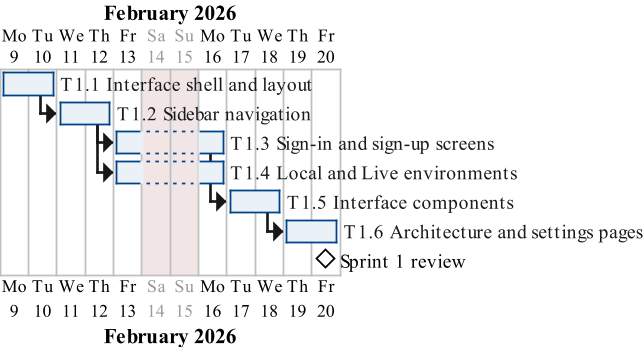
\includegraphics[width=\textwidth,height=0.42\textheight,keepaspectratio]{umls/img/gantt-sprint1.png}
\caption{Sprint 1 schedule (Gantt chart)}
\end{figure}
\figdesc{The chart schedules the foundation work, including interface setup, authentication, navigation, local data, and initial validation.}

\section{Functional Analysis}\label{sumlbl:c5s3}
The main actor in this sprint is the platform user, who can be a sales employee or a manager. The user signs in, lands on the dashboard, moves between the pages, chooses the execution environment, and opens the settings page. The application can run in two environments: a Local one, where the Node.js backend handles the logic and the data, and a Live one, where the backend forwards the request to the n8n workflows. The same interface is used in both, so the experience stays consistent.

\subsection{Use Case Diagram}\label{sumlbl:c5s3ss1}
The figure below presents the use case diagram of this sprint.

\begin{figure}[H]
\centering
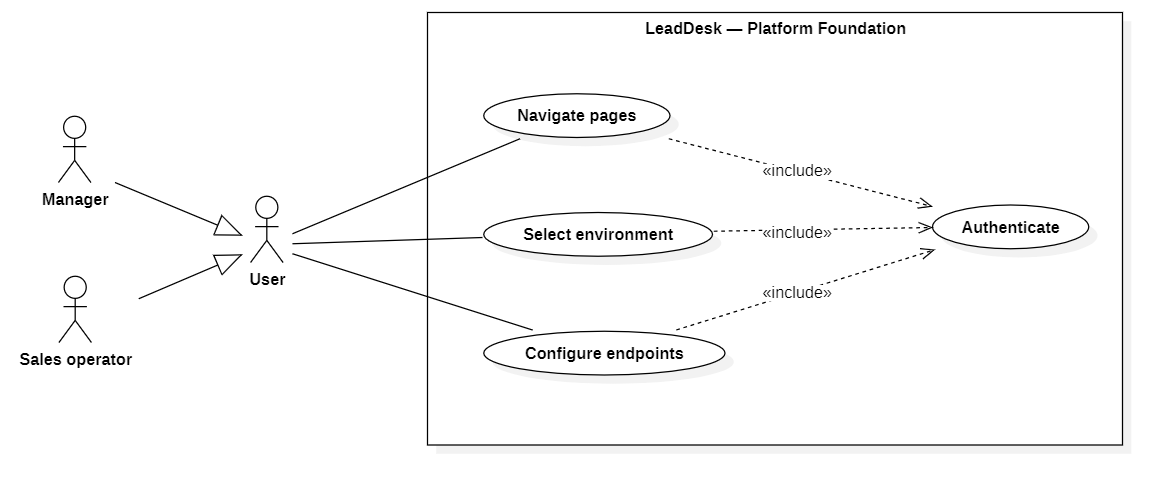
\includegraphics[width=\textwidth,height=0.9\textheight,keepaspectratio]{umls/img/uc-platform-foundation.png}
\caption{Use case diagram of the platform foundation}
\end{figure}
\figdesc{The diagram groups the common platform actions that both operational roles inherit through the general User actor.}

\noindent\textbf{Actor responsibilities.}
\begin{itemize}
\item \textbf{User:} performs the shared actions of navigating pages, selecting the execution environment, and configuring workflow endpoints.
\item \textbf{Manager:} specializes the User role and uses the common foundation while supervising dashboard, follow-up, and configuration activities.
\item \textbf{Sales operator:} specializes the User role and uses the same foundation while carrying out lead capture and daily CRM operations.
\end{itemize}

The two roles, the manager and the sales operator, are generalized into a single \emph{User} actor, because they sign in and use the platform the same way. The authentication use cases are grouped in their own diagram below.

\begin{figure}[H]
\centering
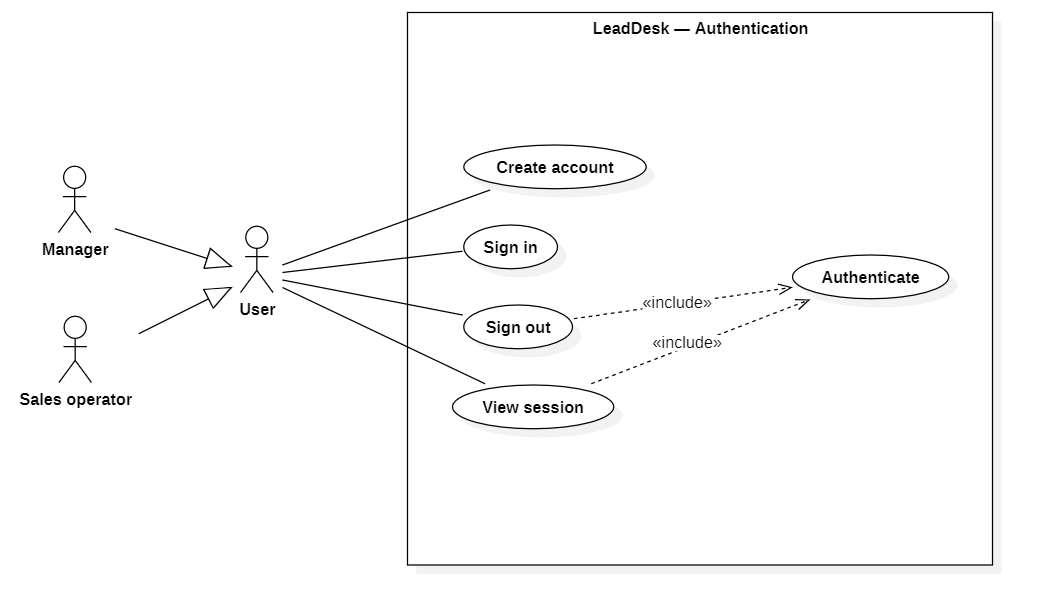
\includegraphics[width=\textwidth,height=0.9\textheight,keepaspectratio]{umls/img/uc-authentication.png}
\caption{Use case diagram of the authentication module}
\end{figure}
\figdesc{The diagram shows the account and session actions that control access to protected platform functions.}

\noindent\textbf{Actor responsibilities.}
\begin{itemize}
\item \textbf{User:} creates an account, signs in, signs out, and restores the active session when the application reloads.
\item \textbf{Manager:} inherits the User authentication behavior before accessing management functions.
\item \textbf{Sales operator:} inherits the User authentication behavior before accessing operational sales functions.
\end{itemize}

A self-service account management area is also planned, so that each user can view their profile and change their username, password, or picture, or delete their account. The diagram below models this planned feature.

\begin{figure}[H]
\centering
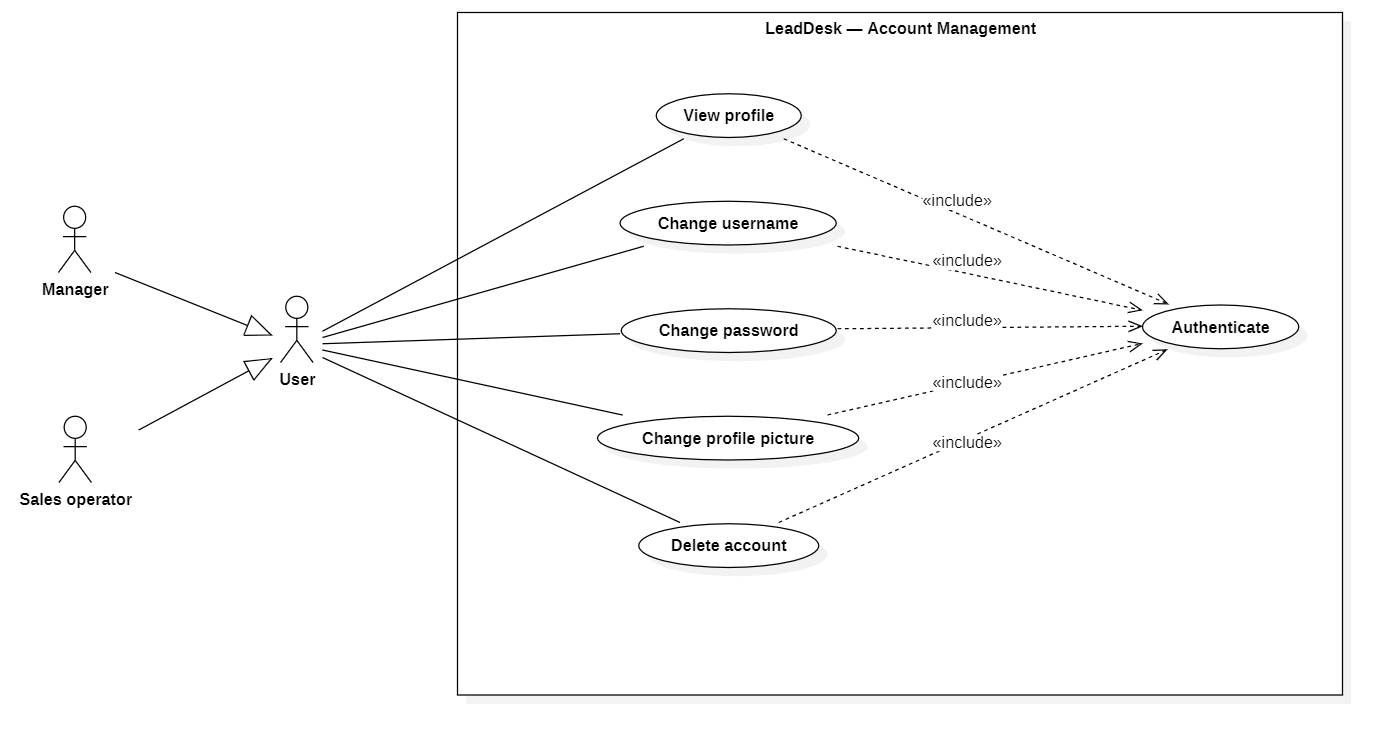
\includegraphics[width=\textwidth,height=0.9\textheight,keepaspectratio]{umls/img/uc-account-management.png}
\caption{Use case diagram of the planned account management module}
\end{figure}
\figdesc{The diagram models the planned self-service actions through which an authenticated user will maintain or remove an account.}

\noindent\textbf{Actor responsibilities.}
\begin{itemize}
\item \textbf{User:} views the profile and requests changes to the username, password, profile picture, or account status.
\item \textbf{Manager:} inherits the User account-management actions for the manager's own profile.
\item \textbf{Sales operator:} inherits the User account-management actions for the sales operator's own profile.
\end{itemize}

\subsection{Use Case Descriptions}\label{sumlbl:c5s3ss2}
The table below describes the use cases shown in the three diagrams above. Here the \emph{User} actor stands for both roles (manager and sales operator), which are generalized into it. The account management use cases are planned and not yet implemented.

\begin{table}[H]
\centering
\small
\begin{tabularx}{\textwidth}{|p{3.9cm}|p{2.2cm}|X|}
\hline\rowcolor{TabHead}
\textbf{Use case} & \textbf{Actor} & \textbf{Description} \\
\hline
Navigate pages & User & Move between the dashboard, capture, workspace, follow-up, assistant, and system pages. \\
\hline
Select environment & User & Choose the Local or Live execution context used by the interface. \\
\hline
Configure endpoints & User & Open the settings page to set and check the workflow endpoints. \\
\hline
Create account & User & Register with a name, an email, and a password; the account gets the Sales role. \\
\hline
Sign in & User & Authenticate with an email and a password to open a session and reach the dashboard. \\
\hline
Sign out & User & Close the current session and return to the sign-in screen. \\
\hline
View session & User & Read the currently signed-in account to restore the session on reload. \\
\hline
Authenticate & System & Guard every protected page and request through the backend session check; included by the protected use cases. \\
\hline
View profile \emph{(planned)} & User & See the current account details. \\
\hline
Change username \emph{(planned)} & User & Update the account name. \\
\hline
Change password \emph{(planned)} & User & Update the account password. \\
\hline
Change profile picture \emph{(planned)} & User & Update the account picture. \\
\hline
Delete account \emph{(planned)} & User & Permanently remove the account. \\
\hline
\end{tabularx}
\caption{Use case descriptions for the platform foundation, authentication, and account management}
\end{table}

\section{Conceptual Modeling}\label{sumlbl:c5s4}
\subsection{Class Diagram}\label{sumlbl:c5s4ssC}
The class diagram below shows the classes involved in this sprint: the user account and the session opened when the user signs in.

\begin{figure}[H]
\centering
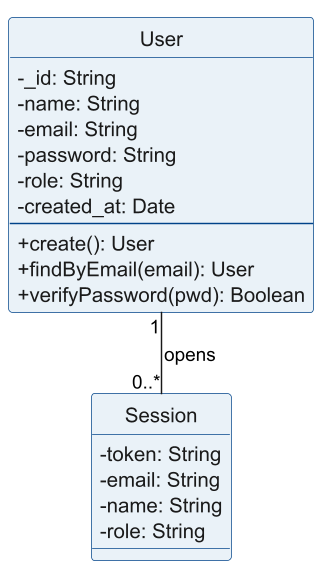
\includegraphics[width=0.8\textwidth,height=0.5\textheight,keepaspectratio]{umls/img/class-auth.png}
\caption{Class diagram of the authentication module}
\end{figure}
\figdesc{The diagram relates the user account to its authenticated session and shows the data required to identify the user and maintain access.}

\subsection{Sequence Diagram}\label{sumlbl:c5s4ss1}
The sign-in flow is the first exchange between the user and the system. The user sends the email and the password to the interface, the interface forwards them to the backend, and the backend checks the stored password before opening a session.

The figure below presents the sequence diagram of the sign-in workflow.

\begin{figure}[H]
\centering
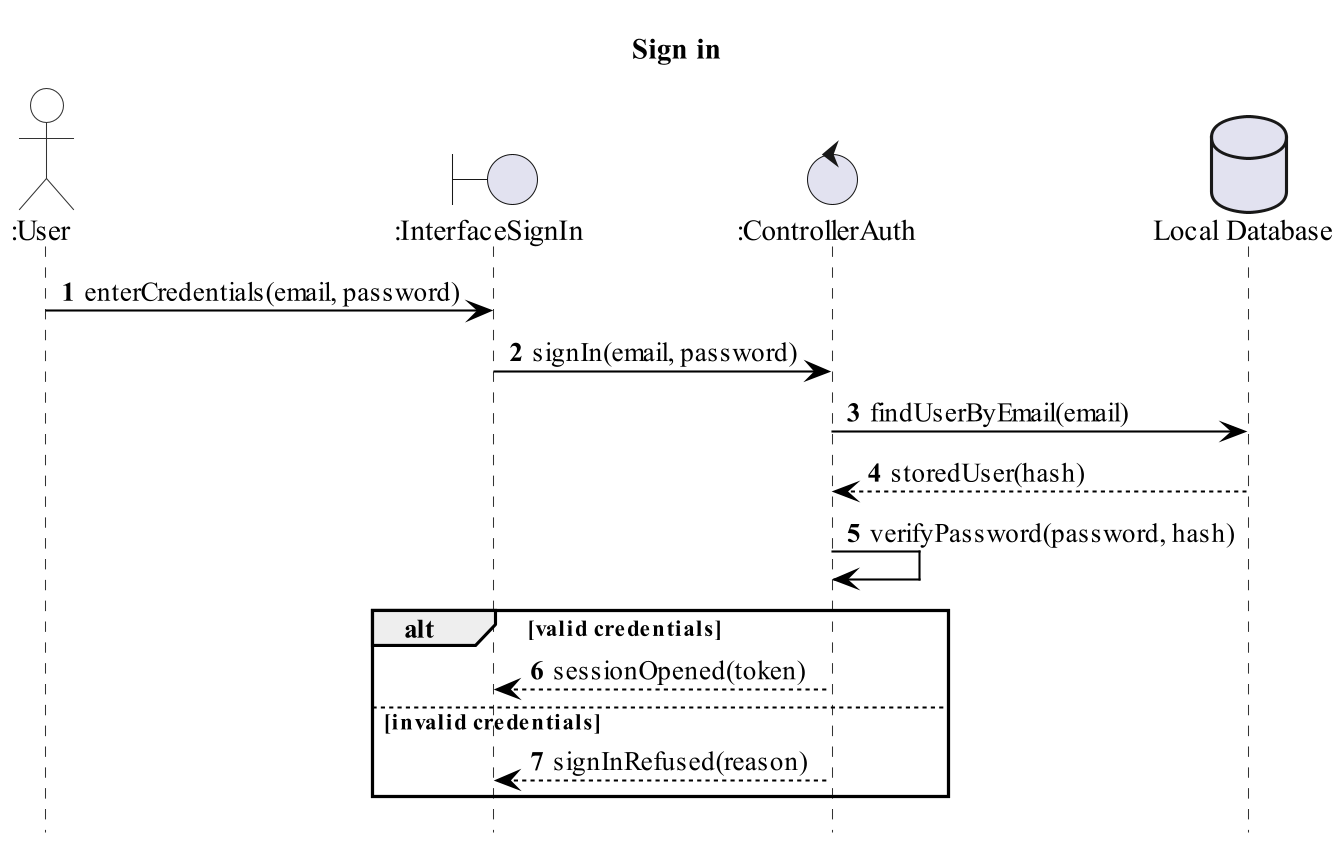
\includegraphics[width=0.92\textwidth,height=0.62\textheight,keepaspectratio]{umls/img/seq-signin.png}
\caption{Sequence diagram of the sign-in workflow}
\end{figure}
\figdesc{The sequence follows credentials from the interface to the backend, through password verification, and back as either a valid session or an authentication error.}

The sequence below shows the sign-up flow, where a visitor creates a new account before signing in for the first time.

\begin{figure}[H]
\centering
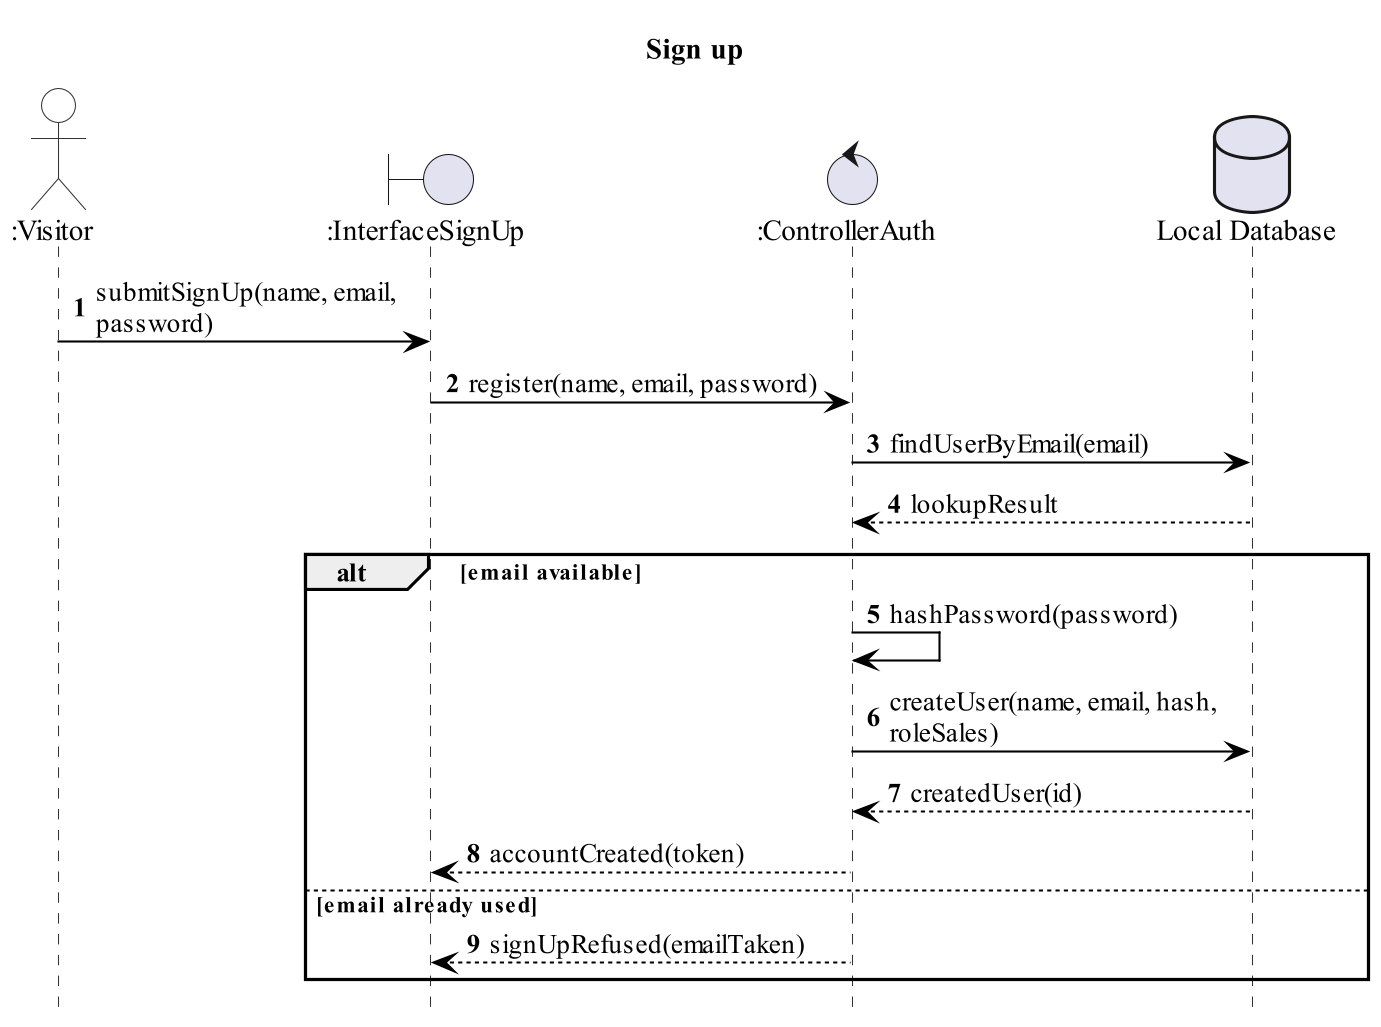
\includegraphics[width=0.92\textwidth,height=0.62\textheight,keepaspectratio]{umls/img/seq-signup.png}
\caption{Sequence diagram of the sign-up (account creation) workflow}
\end{figure}
\figdesc{The sequence shows how registration data is validated, securely stored, and returned as a newly created sales account.}


\section{Realization}\label{sumlbl:c5s5}
The interface follows a modular organization even without a large framework. The constants, the data, and the backend calls sit in the Model. The rendering functions sit in the View. The events and the user actions are handled by the Controller. The visual design uses a professional style with cards, tables, badges, and charts, so the result looks like an operations console rather than a generic landing page. On the backend side, the passwords are hashed with scrypt and the sessions use bearer tokens.

\subsection{Screenshots}\label{sumlbl:c5s5ss1}
The screenshots below show the first results of Sprint 1: the landing page, the sign-in screen, and the main dashboard that becomes the entry point of the application.

\shot{01-landing.png}{Landing page}{This screenshot showcases the landing page. It introduces the platform and its main promise, turning a customer message into a qualified opportunity, and gives the user a clear entry point into the console.}

\shot{03-login.png}{Sign-in screen}{This screenshot showcases the sign-in screen. The user enters an email and a password to open the console, and the demo accounts shown below make the platform easy to test.}

\shot{04-dashboard.png}{Main dashboard (entry point after sign-in)}{This screenshot showcases the main dashboard, which the user reaches right after signing in. The sidebar gives access to every module, and the central area is the working space where the CRM results are displayed.}

\section{Conclusion}\label{sumlbl:c5s6}
Sprint 1 delivered the foundation of the application: the interface, the navigation, the sign-in, and the system pages. These elements made it possible to add the CRM modules in the next sprints without rebuilding the structure.


\chapter{Sprint 2: Lead Capture and Duplicate Detection}

\vspace{0.35cm}
{\Large\bfseries Summary}\par
\vspace{3pt}{\color{black}\hrule height 0.6pt}\vspace{0.30cm}
{\small
\chsummaryitem{6.1}{Introduction}{sumlbl:c6s1}
\chsummaryitem{6.2}{Objectives and Task Identification}{sumlbl:c6s2}
\chsummarysub{6.2.1}{Sprint Objective}{sumlbl:c6s2ss1}
\chsummarysub{6.2.2}{Sprint Backlog}{sumlbl:c6s2ss2}
\chsummaryitem{6.3}{Functional Analysis}{sumlbl:c6s3}
\chsummarysub{6.3.1}{Use Case Diagram}{sumlbl:c6s3ss1}
\chsummarysub{6.3.2}{Use Case Descriptions}{sumlbl:c6s3ss2}
\chsummaryitem{6.4}{Conceptual Modeling}{sumlbl:c6s4}
\chsummarysub{6.4.1}{Class Diagram}{sumlbl:c6s4ssC}
\chsummarysub{6.4.2}{Sequence Diagram}{sumlbl:c6s4ss1}
\chsummaryitem{6.5}{Realization}{sumlbl:c6s5}
\chsummarysub{6.5.1}{Screenshots}{sumlbl:c6s5ss1}
\chsummaryitem{6.6}{Conclusion}{sumlbl:c6s6}
}
\clearpage

\section{Introduction}\label{sumlbl:c6s1}
The second sprint built one of the most important features of the platform: lead capture. The goal was to let a sales operator type a normal customer message and turn it into clean CRM data. This feature is central because it shows the practical value of AI in the project.

\section{Objectives and Task Identification}\label{sumlbl:c6s2}
\subsection{Sprint Objective}\label{sumlbl:c6s2ss1}
The goal of Sprint 2 was to reduce manual data entry and to improve data quality. A customer may write a message that contains a name, an email, a phone number, an interest, and an urgency. Instead of copying each field by hand, the system reads the message and fills the fields. The workflow also checks whether the email or the phone already exists in the CRM before creating a new opportunity.

\subsection{Sprint Backlog}\label{sumlbl:c6s2ss2}
The table below lists the tasks planned for this sprint.

\begin{table}[H]
\centering
\small
\begin{tabularx}{\textwidth}{|p{1.4cm}|X|p{2cm}|p{2cm}|}
\hline\rowcolor{TabHead}
\textbf{ID} & \textbf{Task} & \textbf{Priority} & \textbf{Status} \\
\hline
T2.1 & Build the lead capture form in the interface & Critical & Done \\
\hline
T2.3 & Create the backend capture service and the capture history & Critical & Done \\
\hline
T2.4 & Set up the n8n lead capture workflow & Critical & Done \\
\hline
T2.5 & Add duplicate detection by email and phone & Critical & Done \\
\hline
T2.2 & Implement the local field extraction logic & High & Done \\
\hline
T2.6 & Show the created or duplicate result clearly & High & Done \\
\hline
\end{tabularx}
\caption{Sprint 2 backlog}
\end{table}

The Gantt chart below shows the schedule of the tasks planned for this sprint.
\begin{figure}[H]
\centering
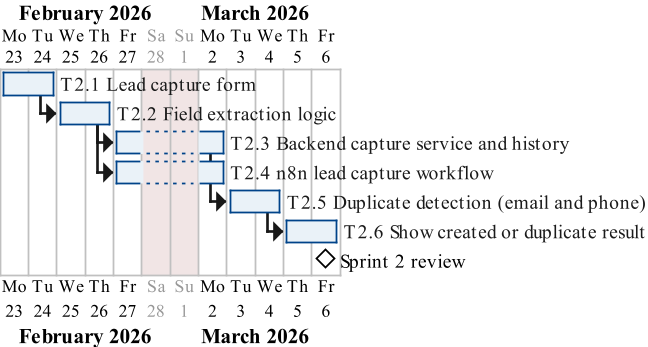
\includegraphics[width=\textwidth,height=0.42\textheight,keepaspectratio]{umls/img/gantt-sprint2.png}
\caption{Sprint 2 schedule (Gantt chart)}
\end{figure}
\figdesc{The chart organizes the lead-capture sprint from message extraction and duplicate detection through opportunity creation, workspace listing, and tests.}

\section{Functional Analysis}\label{sumlbl:c6s3}
The capture process starts when the sales operator receives a customer message. The message can be informal and may hold the information in any order. The system reads a name when possible, an email, a phone number, an interest, an intent, a priority, and a recommended action, then shows the result to the user. The duplicate check is essential: a CRM with repeated opportunities becomes hard to manage. The workflow compares the new email and phone with the opportunities already in Odoo, returns a duplicate result when a match is found, and creates a new opportunity when there is none.

\subsection{Use Case Diagram}\label{sumlbl:c6s3ss1}
The figure below presents the use case diagram of this sprint.

\begin{figure}[H]
\centering
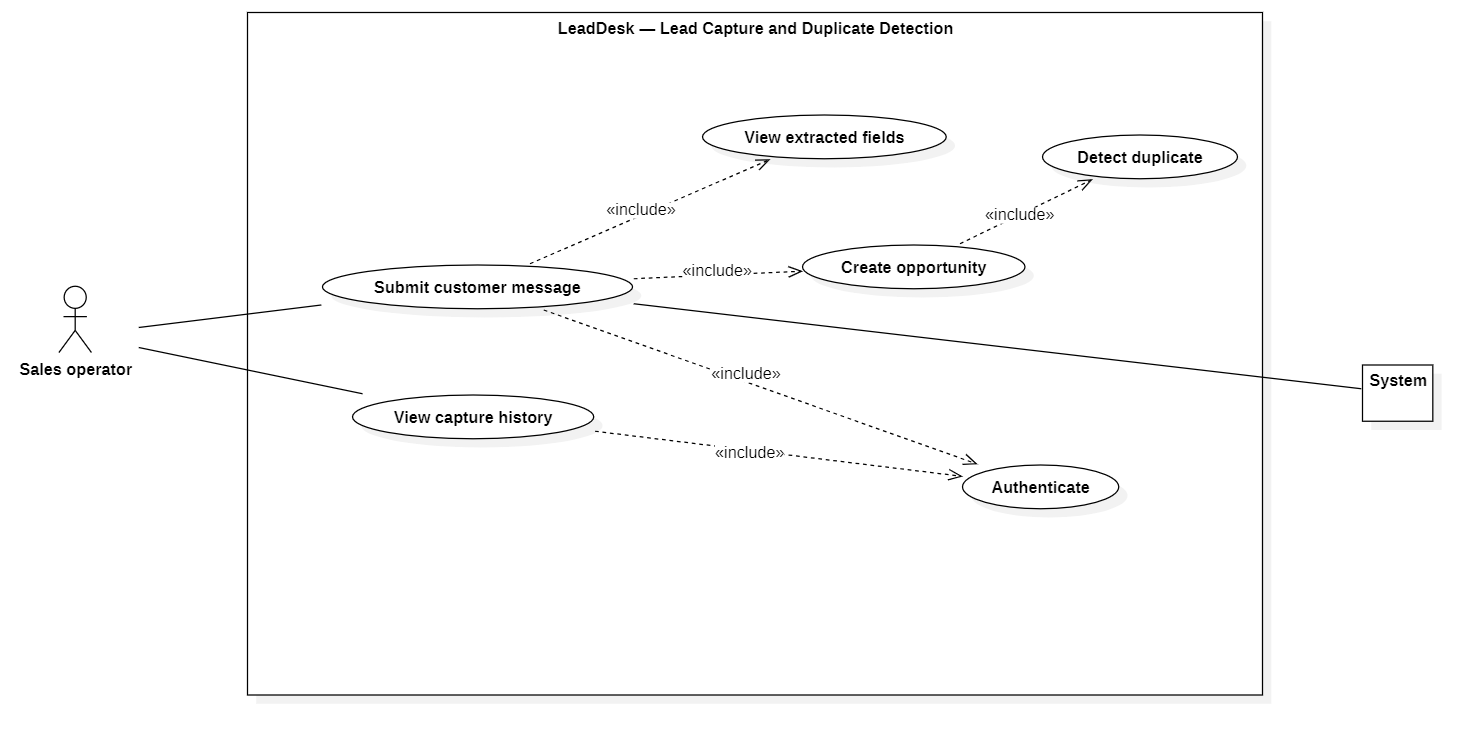
\includegraphics[width=\textwidth,height=0.9\textheight,keepaspectratio]{umls/img/uc-lead-capture.png}
\caption{Use case diagram of the lead capture module}
\end{figure}
\figdesc{The diagram connects the sales operator's capture actions with the automated CRM processing performed by the system.}

\noindent\textbf{Actor responsibilities.}
\begin{itemize}
\item \textbf{Sales operator:} submits the customer message, reviews the extracted information, and consults the capture history and result.
\item \textbf{System:} authenticates the request, extracts structured fields, compares the lead with existing CRM records, and creates the opportunity only when no duplicate exists.
\end{itemize}

\subsection{Use Case Descriptions}\label{sumlbl:c6s3ss2}
The table below describes the use cases shown in the diagram above.

\begin{table}[H]
\centering
\small
\begin{tabularx}{\textwidth}{|p{3.6cm}|p{2.2cm}|X|}
\hline\rowcolor{TabHead}
\textbf{Use case} & \textbf{Actor} & \textbf{Description} \\
\hline
Submit customer message & Sales operator & Paste a free-text customer message into the capture form. \\
\hline
View extracted fields & Sales operator & See the name, email, phone, interest, intent, and priority read from the message. \\
\hline
Create opportunity & System & Save a new opportunity in the CRM when the lead is new. \\
\hline
Detect duplicate & System & Compare the email and phone with existing records and avoid repeated opportunities. \\
\hline
View capture history & Sales operator & Browse the list of past captures and their results. \\
\hline
Authenticate & System & Guard every capture action through the backend session check; included by the use cases above. \\
\hline
\end{tabularx}
\caption{Use case descriptions for the lead capture module}
\end{table}

\section{Conceptual Modeling}\label{sumlbl:c6s4}
\subsection{Class Diagram}\label{sumlbl:c6s4ssC}
The class diagram below shows the classes involved in lead capture: the capture record, the fields extracted from the customer message, and the opportunity it can create.

\begin{figure}[H]
\centering
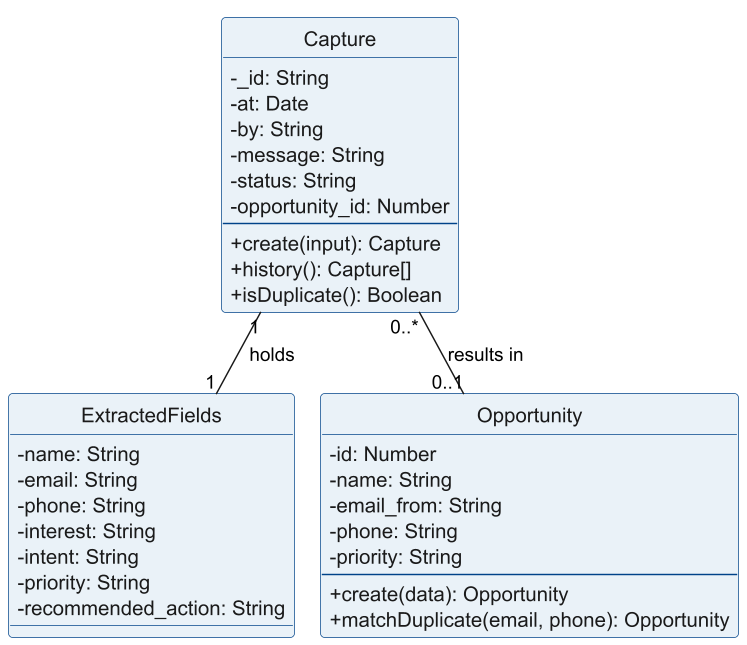
\includegraphics[width=0.8\textwidth,height=0.5\textheight,keepaspectratio]{umls/img/class-capture.png}
\caption{Class diagram of the lead capture module}
\end{figure}
\figdesc{The diagram links the original capture record to its extracted fields and to the CRM opportunity produced when validation succeeds.}

\subsection{Sequence Diagram}\label{sumlbl:c6s4ss1}
The sequence diagram below shows the full exchange, from the customer message to the created or duplicate result. The model reads the fields, a code step validates them, and the duplicate decision is made by code rather than by the model.

\begin{figure}[H]
\centering
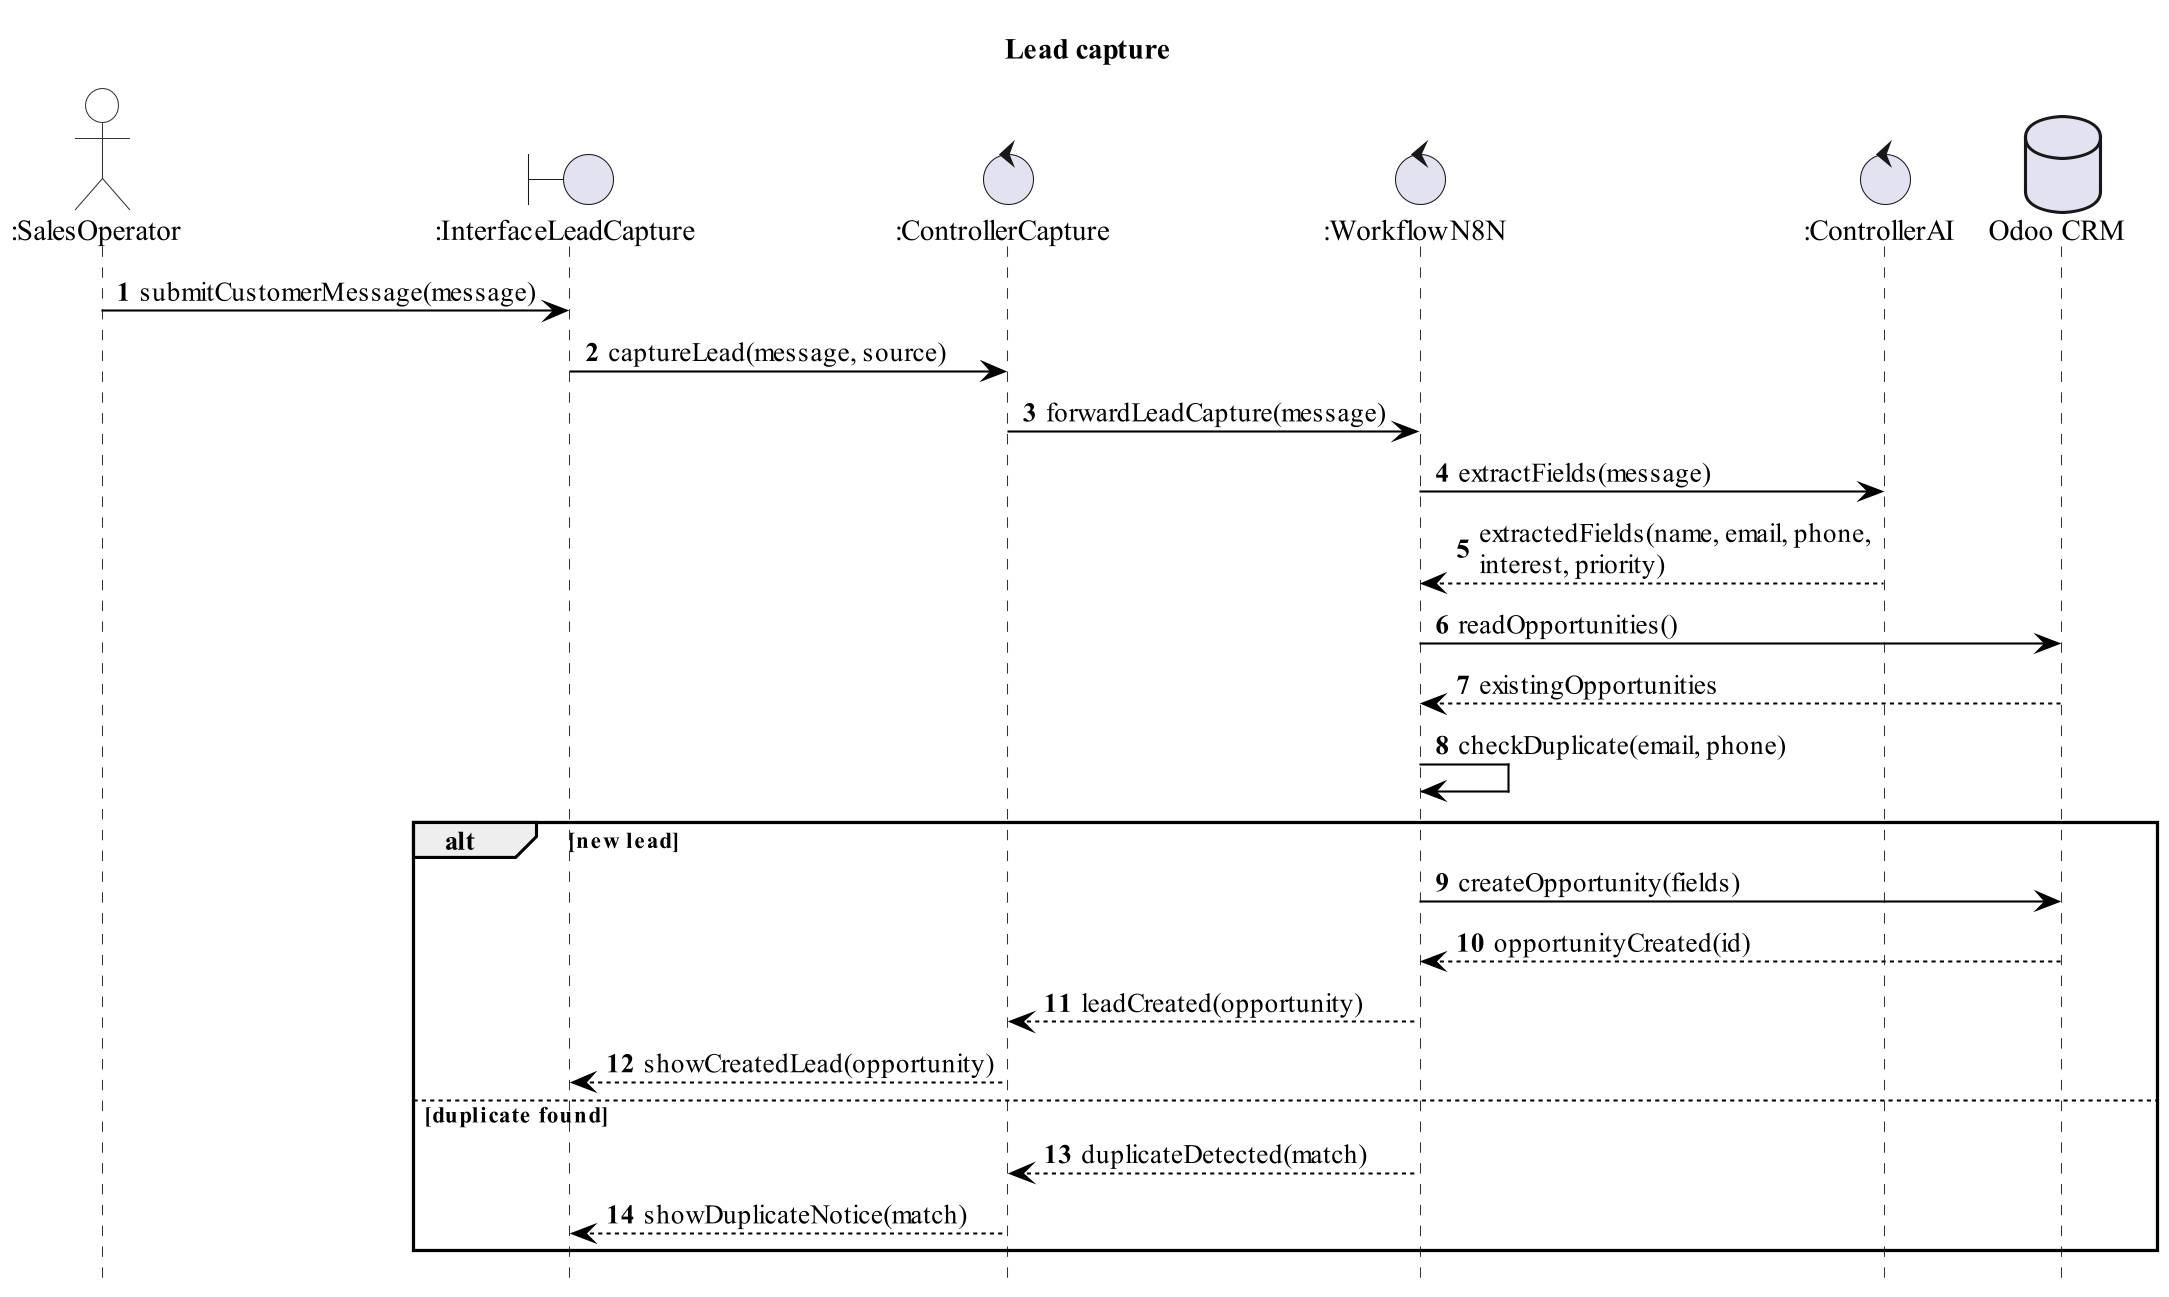
\includegraphics[width=0.92\textwidth,height=0.62\textheight,keepaspectratio]{umls/img/seq-lead-capture.png}
\caption{Sequence diagram of the lead capture and duplicate detection workflow}
\end{figure}
\figdesc{The sequence traces a customer message through extraction, duplicate comparison, conditional CRM creation, and the final status returned to the operator.}

The workspace also lists the existing opportunities. The sequence below shows the read-only lead listing flow that feeds the workspace.

\begin{figure}[H]
\centering
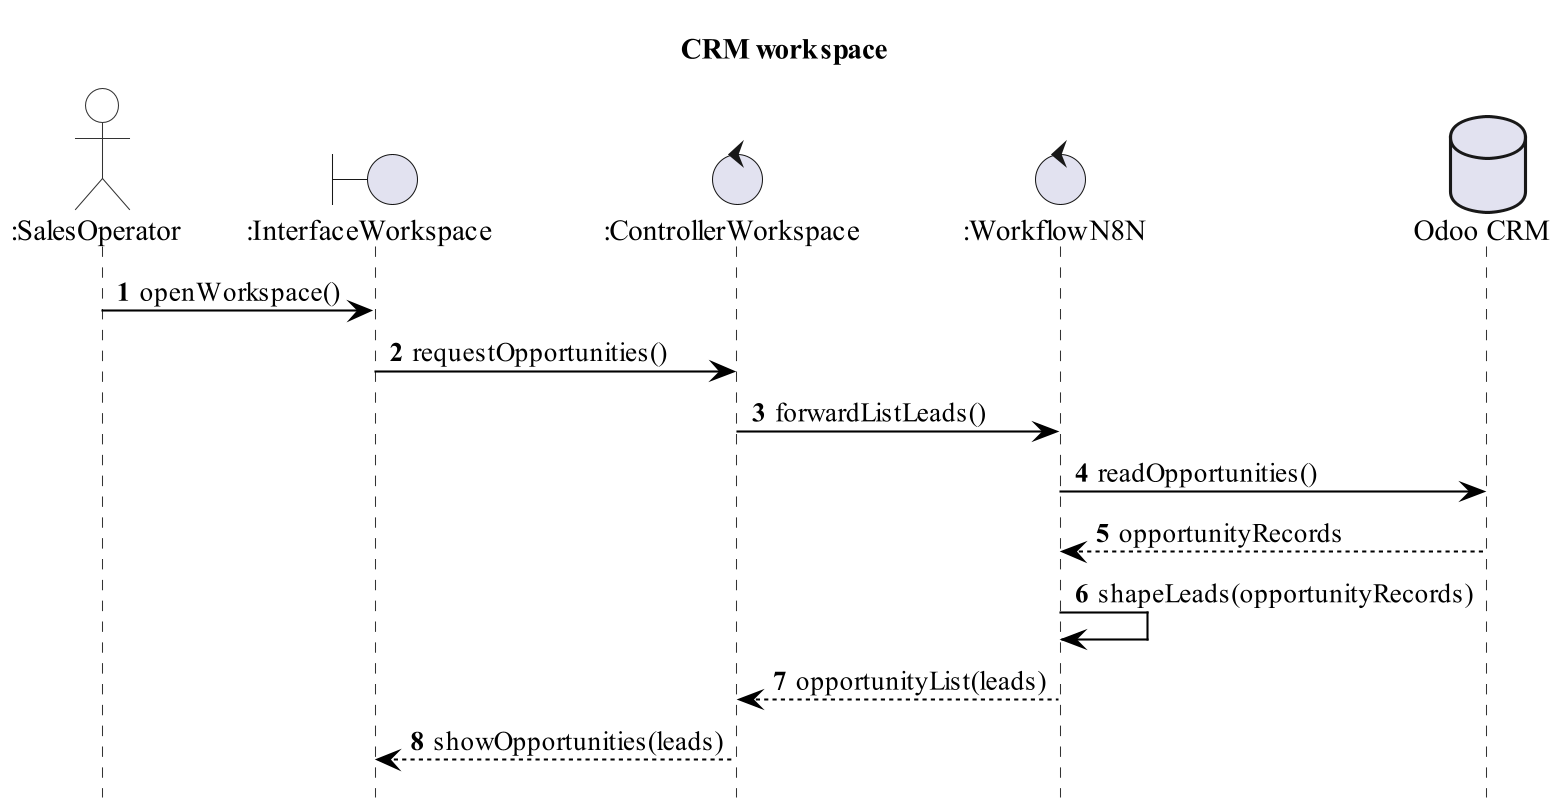
\includegraphics[width=0.92\textwidth,height=0.62\textheight,keepaspectratio]{umls/img/seq-list-leads.png}
\caption{Sequence diagram of the workspace lead listing workflow}
\end{figure}
\figdesc{The sequence shows the authenticated, read-only request used to retrieve, shape, and display opportunities in the workspace.}


\section{Realization}\label{sumlbl:c6s5}
The local environment offers the same feature. The capture service receives a message, reads the useful fields, prepares an opportunity, calls the opportunity service, and writes a capture record for the history. This means the user can test lead capture even when n8n or Odoo is not running. The front end shows the extracted fields and the final status: a created lead with its structured data, or a clear duplicate notice that explains why no new record was created.

\subsection{Screenshots}\label{sumlbl:c6s5ss1}
The screenshots below show the two capture cases and the workspace where the captured leads are listed.

\shot{06-capture-created.png}{Lead capture: opportunity created}{This screenshot showcases a successful capture. The operator pastes a raw customer message, the AI extraction fills the structured fields, and the panel confirms that a new opportunity was created in the CRM.}

\shot{07-capture-duplicate.png}{Lead capture: duplicate detected}{This screenshot showcases the duplicate protection. When the email or the phone already exists, the system stops the creation and shows a clear duplicate notice instead of adding a repeated record.}

\shot{08-workspace.png}{Lead workspace}{This screenshot showcases the lead workspace, where the captured opportunities are listed. The operator can browse the leads and open one of them to read its detailed information.}

\section{Conclusion}\label{sumlbl:c6s6}
Sprint 2 delivered the lead capture feature and the duplicate detection. This sprint showed that AI can reduce manual entry while code protects the integrity of the CRM data. The next sprint focuses on analytics and follow-up.


\chapter{Sprint 3: Analytics and Smart Follow-Up}

\vspace{0.35cm}
{\Large\bfseries Summary}\par
\vspace{3pt}{\color{black}\hrule height 0.6pt}\vspace{0.30cm}
{\small
\chsummaryitem{7.1}{Introduction}{sumlbl:c7s1}
\chsummaryitem{7.2}{Objectives and Task Identification}{sumlbl:c7s2}
\chsummarysub{7.2.1}{Sprint Objective}{sumlbl:c7s2ss1}
\chsummarysub{7.2.2}{Sprint Backlog}{sumlbl:c7s2ss2}
\chsummaryitem{7.3}{Functional Analysis}{sumlbl:c7s3}
\chsummarysub{7.3.1}{Use Case Diagram}{sumlbl:c7s3ss1}
\chsummarysub{7.3.2}{Use Case Descriptions}{sumlbl:c7s3ss2}
\chsummaryitem{7.4}{Conceptual Modeling}{sumlbl:c7s4}
\chsummarysub{7.4.1}{Class Diagram}{sumlbl:c7s4ssC}
\chsummarysub{7.4.2}{Sequence Diagrams}{sumlbl:c7s4ss1}
\chsummaryitem{7.5}{Realization}{sumlbl:c7s5}
\chsummarysub{7.5.1}{Screenshots}{sumlbl:c7s5ss1}
\chsummaryitem{7.6}{Conclusion}{sumlbl:c7s6}
}
\clearpage

\section{Introduction}\label{sumlbl:c7s1}
After lead capture, the next step was to give the team and the manager more visibility. Sprint 3 built the CRM analytics and the smart follow-up. These features read the CRM records to show the state of the pipeline and to help the team contact quiet leads.

\section{Objectives and Task Identification}\label{sumlbl:c7s2}
\subsection{Sprint Objective}\label{sumlbl:c7s2ss1}
The goal of Sprint 3 was to turn raw opportunities into useful information. A manager does not only need a table of leads. The manager needs to know how large the pipeline is, how complete the contact data is, and how active the leads are. The sales employee also needs help deciding which leads to contact.

\subsection{Sprint Backlog}\label{sumlbl:c7s2ss2}
The table below lists the tasks planned for this sprint.

\begin{table}[H]
\centering
\small
\begin{tabularx}{\textwidth}{|p{1.4cm}|X|p{2cm}|p{2cm}|}
\hline\rowcolor{TabHead}
\textbf{ID} & \textbf{Task} & \textbf{Priority} & \textbf{Status} \\
\hline
T3.1 & Compute the CRM indicators from the opportunity records & Critical & Done \\
\hline
T3.4 & Detect inactive opportunities after seven days & Critical & Done \\
\hline
T3.2 & Create the dashboard cards and charts & High & Done \\
\hline
T3.3 & Generate a readable manager summary & High & Done \\
\hline
T3.5 & Generate follow-up messages & High & Done \\
\hline
T3.6 & Present the follow-up results in the interface & High & Done \\
\hline
\end{tabularx}
\caption{Sprint 3 backlog}
\end{table}

The Gantt chart below shows the schedule of the tasks planned for this sprint.
\begin{figure}[H]
\centering
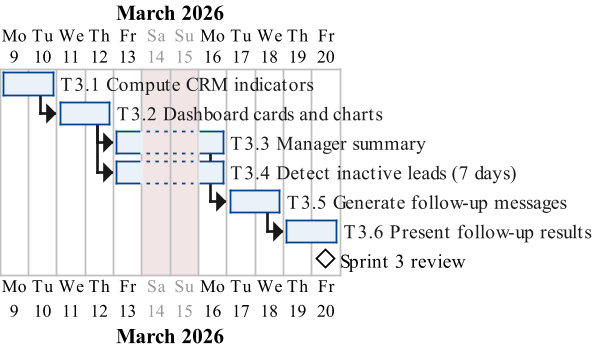
\includegraphics[width=\textwidth,height=0.42\textheight,keepaspectratio]{umls/img/gantt-sprint3.png}
\caption{Sprint 3 schedule (Gantt chart)}
\end{figure}
\figdesc{The chart schedules dashboard indicators, analytical summaries, inactivity detection, follow-up drafting, and their integration tests.}

\section{Functional Analysis}\label{sumlbl:c7s3}
This sprint serves two actors. The manager opens the dashboard, reads the indicators, and asks for a written summary of the pipeline. The sales operator opens the follow-up center, where the system detects the inactive leads and drafts a message for each one. The indicators are computed by code, and the model is used only to turn the finished numbers into a readable summary and to draft the follow-up messages.

\subsection{Use Case Diagram}\label{sumlbl:c7s3ss1}
The figure below presents the use case diagram of this sprint.

\begin{figure}[H]
\centering
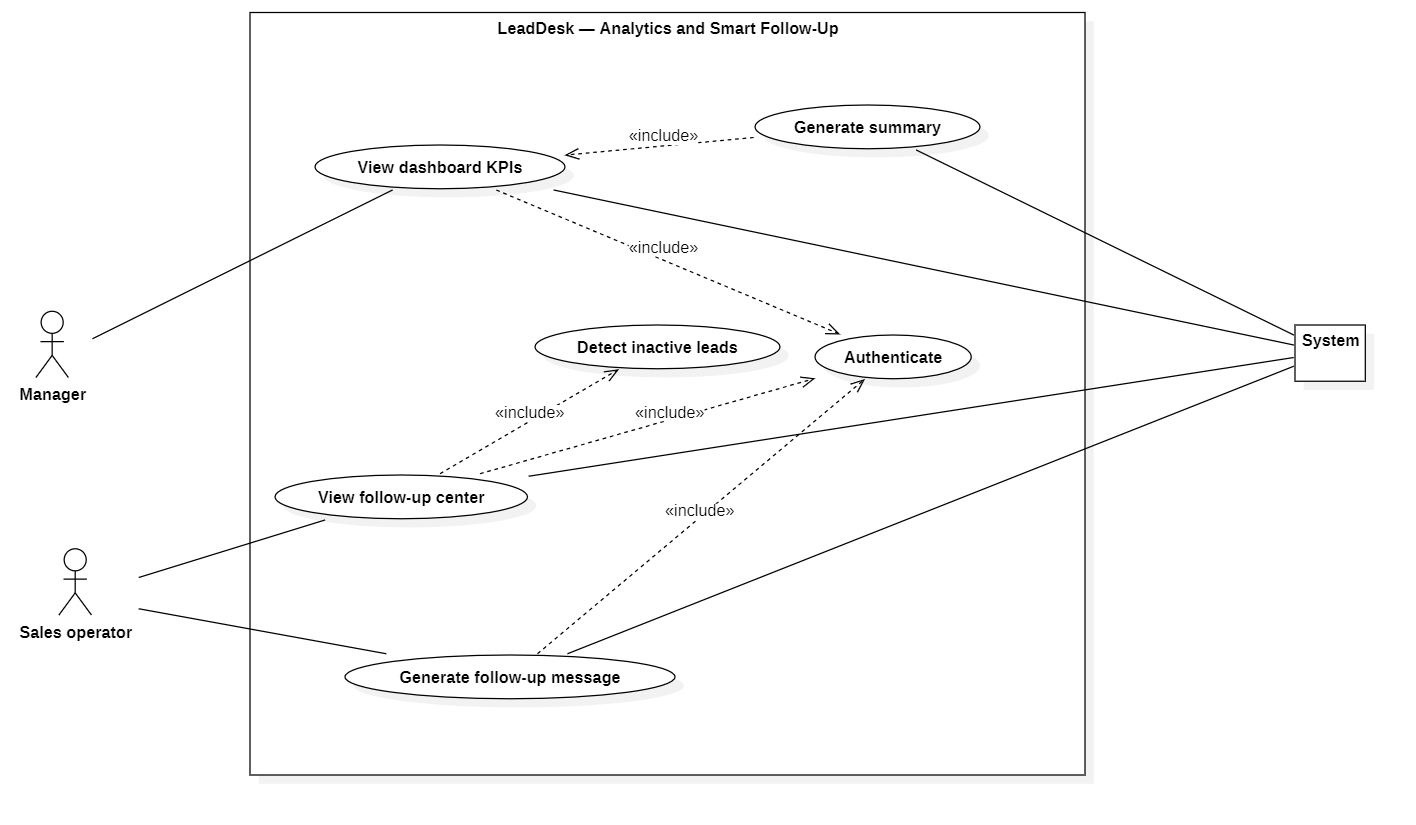
\includegraphics[width=\textwidth,height=0.9\textheight,keepaspectratio]{umls/img/uc-analytics-followup.png}
\caption{Use case diagram of the analytics and follow-up module}
\end{figure}
\figdesc{The diagram separates the manager's analytical tasks from the sales operator's follow-up tasks while showing the automation that supports both roles.}

\noindent\textbf{Actor responsibilities.}
\begin{itemize}
\item \textbf{Manager:} views pipeline KPIs and requests a written summary to supervise CRM activity and identify priorities.
\item \textbf{Sales operator:} opens the follow-up center, reviews inactive opportunities, and uses the generated messages to prepare renewed contact.
\item \textbf{System:} authenticates requests, computes indicators, detects leads inactive for at least seven days, and drafts the summaries and follow-up messages returned to users.
\end{itemize}

\subsection{Use Case Descriptions}\label{sumlbl:c7s3ss2}
The table below describes the use cases shown in the diagram above.

\begin{table}[H]
\centering
\small
\begin{tabularx}{\textwidth}{|p{3.8cm}|p{2.2cm}|X|}
\hline\rowcolor{TabHead}
\textbf{Use case} & \textbf{Actor} & \textbf{Description} \\
\hline
View dashboard KPIs & Manager & See the pipeline indicators as cards and charts. \\
\hline
Generate summary & Manager & Ask for a short written summary based on the computed numbers. \\
\hline
Detect inactive leads & System & Find opportunities whose last update is seven days old or more. \\
\hline
Generate follow-up message & Sales operator & Draft a polite message for each inactive lead. \\
\hline
View follow-up center & Sales operator & Review the inactive leads and their drafted messages. \\
\hline
Authenticate & System & Guard every analytics and follow-up action through the backend session check; included by the use cases above. \\
\hline
\end{tabularx}
\caption{Use case descriptions for the analytics and follow-up module}
\end{table}

\section{Conceptual Modeling}\label{sumlbl:c7s4}
\subsection{Class Diagram}\label{sumlbl:c7s4ssC}
The class diagram below shows the classes involved in analytics and follow-up: the opportunity, the KPI summary computed from the pipeline, and the follow-up drafted for an inactive lead.

\begin{figure}[H]
\centering
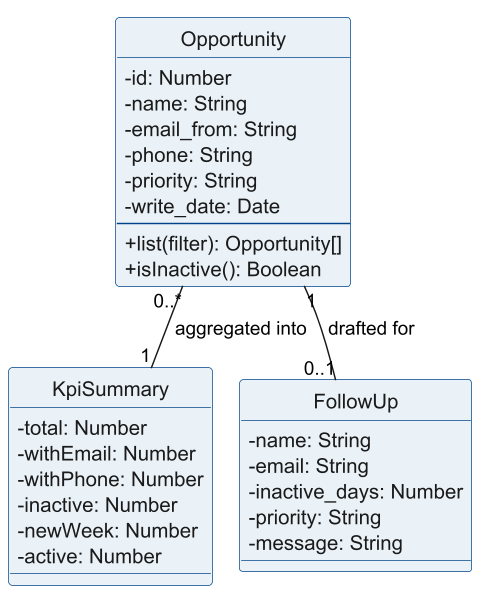
\includegraphics[width=0.8\textwidth,height=0.5\textheight,keepaspectratio]{umls/img/class-analytics.png}
\caption{Class diagram of the analytics and follow-up module}
\end{figure}
\figdesc{The diagram connects opportunities to the computed KPI summary and to follow-up drafts created for records that meet the inactivity rule.}

\subsection{Sequence Diagrams}\label{sumlbl:c7s4ss1}
The first sequence diagram shows how the analytics summary is produced when the dashboard is opened: the numbers are computed by code, and the model only writes the summary.

\begin{figure}[H]
\centering
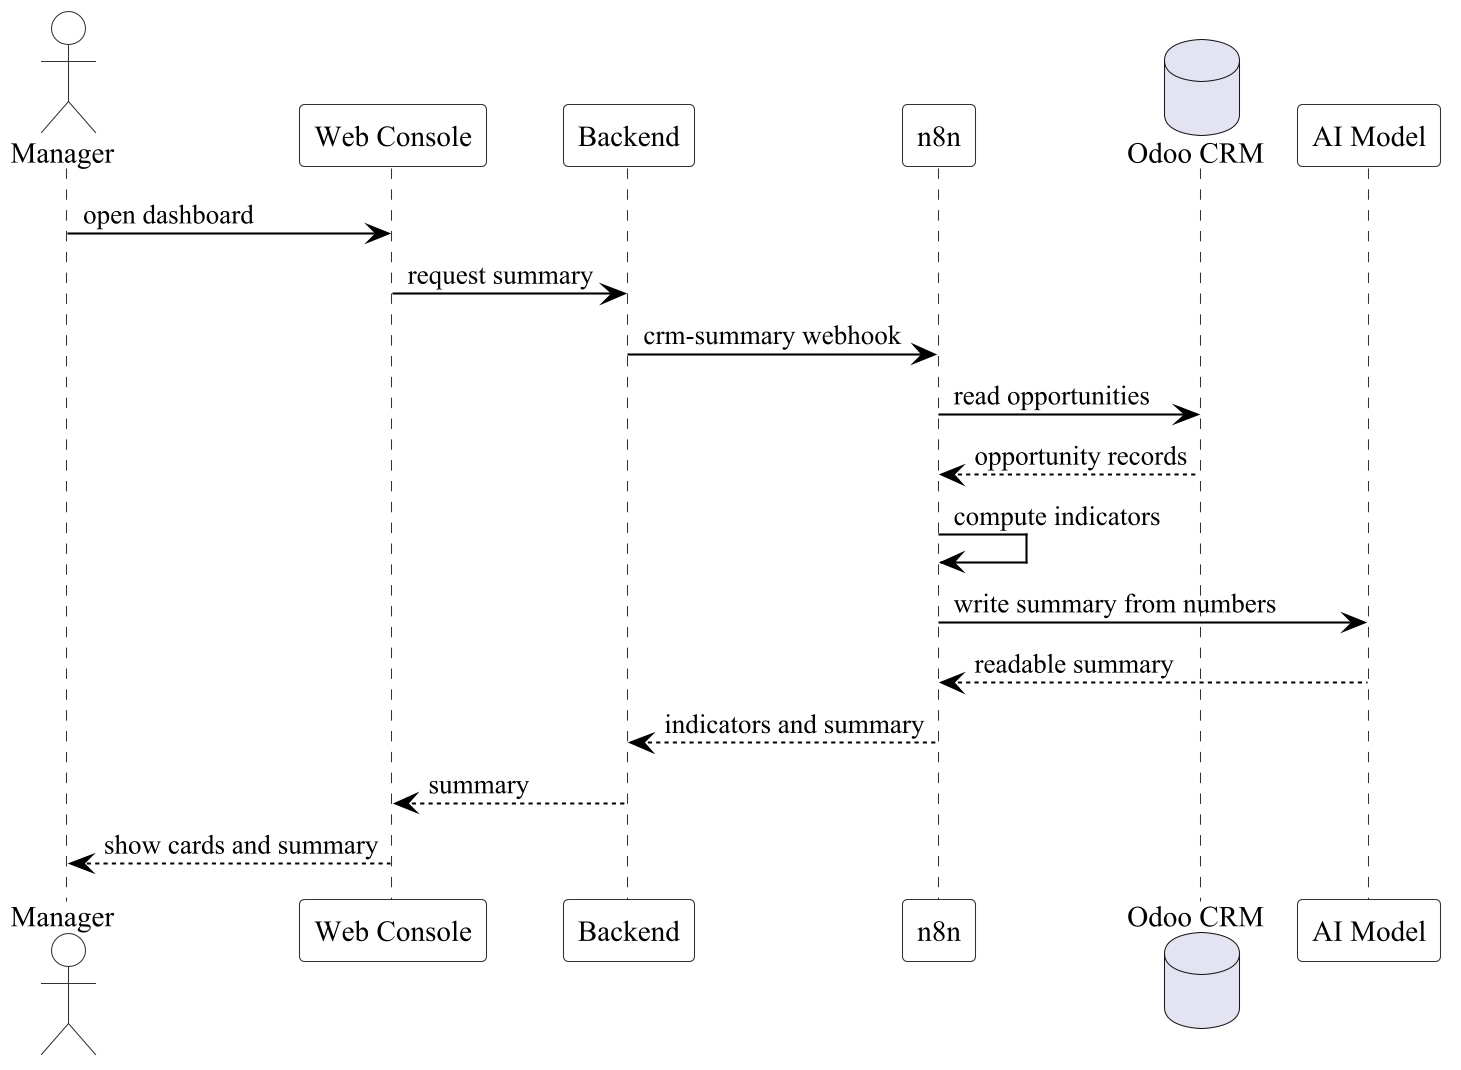
\includegraphics[width=0.92\textwidth,height=0.62\textheight,keepaspectratio]{umls/img/seq-analytics.png}
\caption{Sequence diagram of the CRM analytics summary workflow}
\end{figure}
\figdesc{The sequence shows CRM records being retrieved, converted into deterministic indicators, summarized in readable text, and returned to the manager.}

The second sequence diagram shows the smart follow-up, from the user request to the saved message.

\begin{figure}[H]
\centering
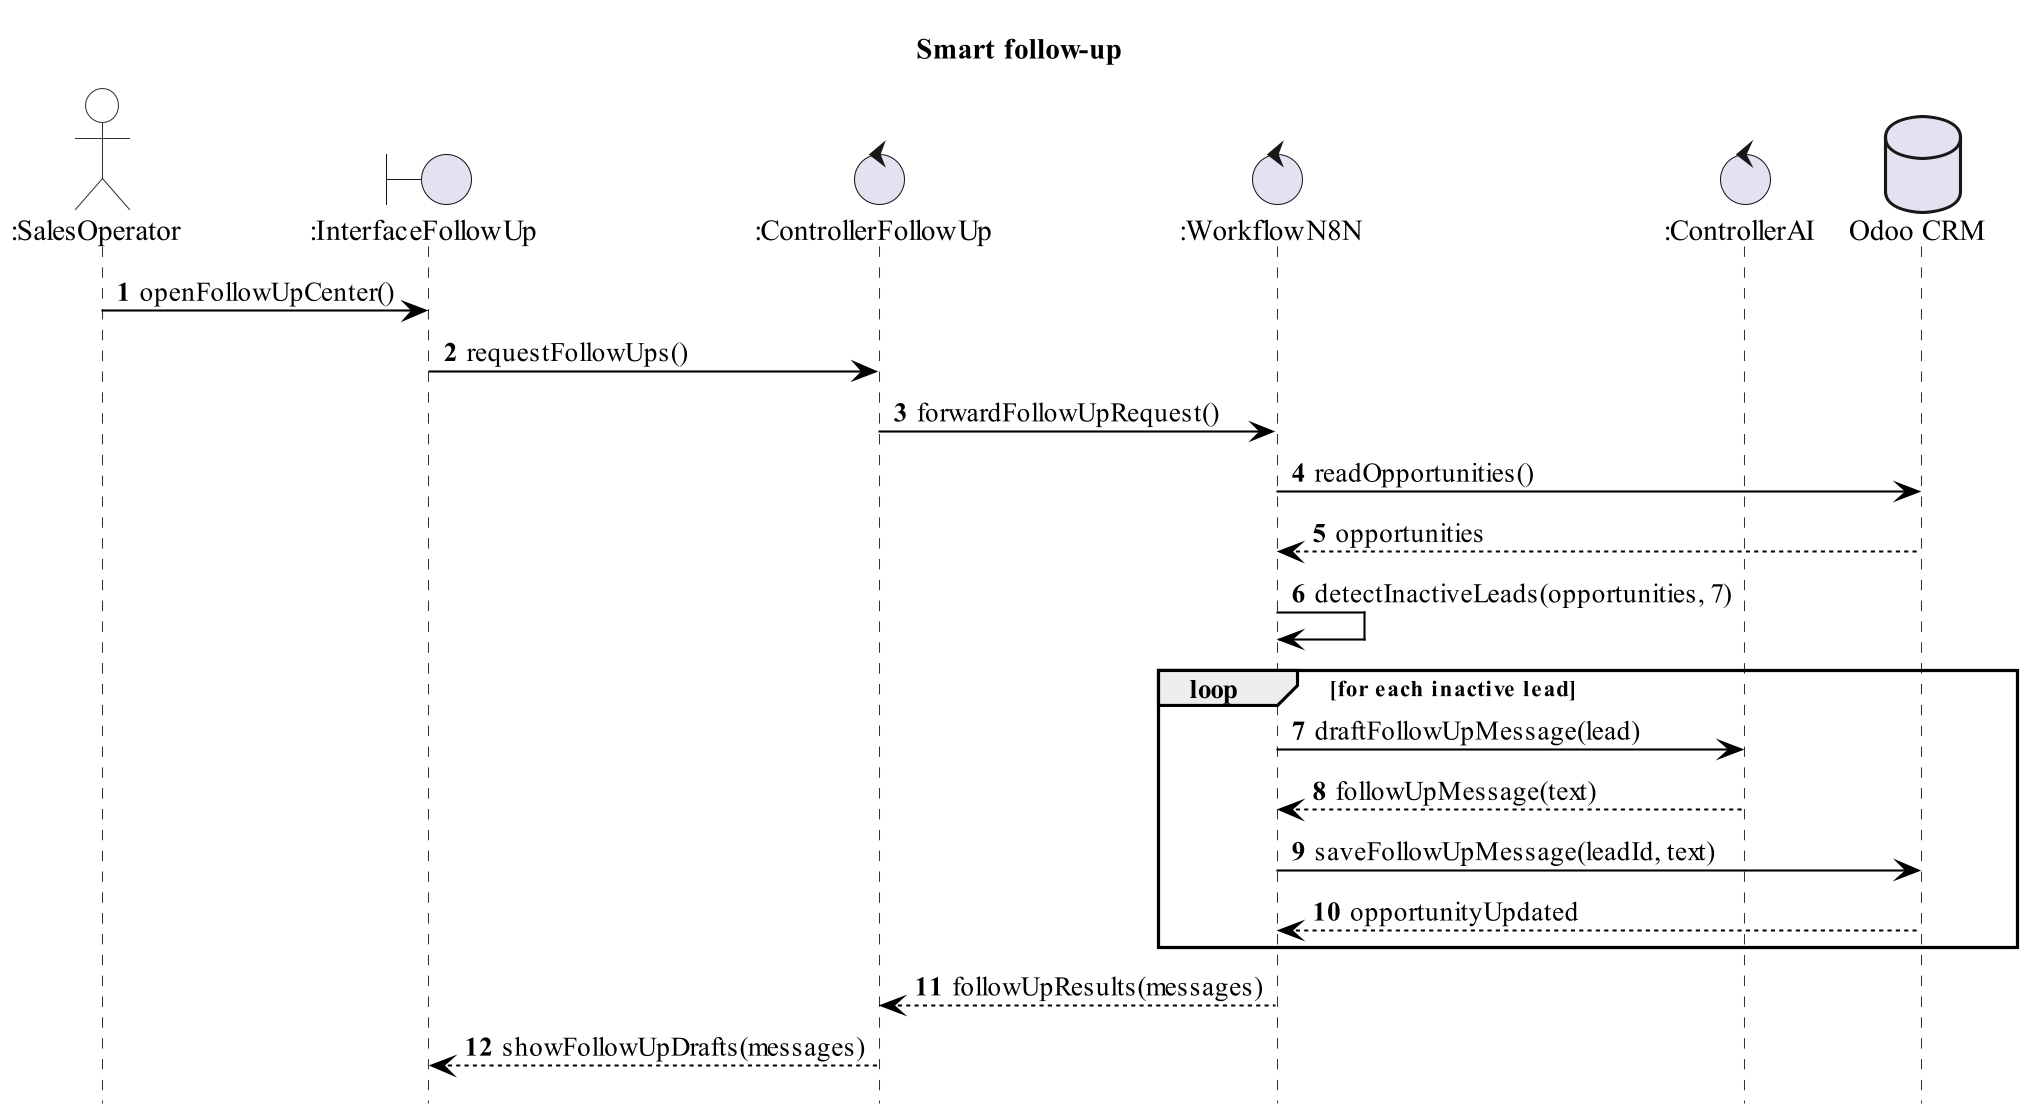
\includegraphics[width=0.92\textwidth,height=0.62\textheight,keepaspectratio]{umls/img/seq-followup.png}
\caption{Sequence diagram of the smart follow-up workflow}
\end{figure}
\figdesc{The sequence follows inactive-lead detection, message generation, optional CRM update, and presentation of the drafts to the sales operator.}


\section{Realization}\label{sumlbl:c7s5}
The dashboard and the follow-up center were built in the interface. The dashboard shows the indicator cards and the charts. The follow-up center shows the inactive leads and the drafted messages. In the local environment, the backend computes the result; in the live environment, the matching n8n workflows are called through the backend proxy. The work also needed careful date handling, because the inactive days depend on the difference between the current date and the last update date.

\subsection{Screenshots}\label{sumlbl:c7s5ss1}
The screenshots below show the analytics dashboard and the follow-up center delivered in this sprint.

\shot{05-dashboard-analytics.png}{Analytics dashboard with AI summary}{This screenshot showcases the analytics dashboard. The cards and charts summarize the pipeline, and the AI analytics summary turns the computed indicators into a short readable review for the manager.}

\shot{10-followup.png}{Follow-up center}{This screenshot showcases the follow-up center. The system detects the inactive leads and drafts a ready-to-send message for each one, so the sales team can re-engage quiet contacts quickly.}

\section{Conclusion}\label{sumlbl:c7s6}
Sprint 3 added value for both managers and sales employees. Managers receive readable summaries, and sales employees receive ready follow-up drafts. The next sprint focuses on the CRM assistant and the live integration.


\chapter{Sprint 4: CRM Assistant and Live Integration}

\vspace{0.35cm}
{\Large\bfseries Summary}\par
\vspace{3pt}{\color{black}\hrule height 0.6pt}\vspace{0.30cm}
{\small
\chsummaryitem{8.1}{Introduction}{sumlbl:c8s1}
\chsummaryitem{8.2}{Objectives and Task Identification}{sumlbl:c8s2}
\chsummarysub{8.2.1}{Sprint Objective}{sumlbl:c8s2ss1}
\chsummarysub{8.2.2}{Sprint Backlog}{sumlbl:c8s2ss2}
\chsummaryitem{8.3}{Functional Analysis}{sumlbl:c8s3}
\chsummarysub{8.3.1}{Use Case Diagram}{sumlbl:c8s3ss1}
\chsummarysub{8.3.2}{Use Case Descriptions}{sumlbl:c8s3ss2}
\chsummaryitem{8.4}{Conceptual Modeling}{sumlbl:c8s4}
\chsummarysub{8.4.1}{Class Diagram}{sumlbl:c8s4ssC}
\chsummarysub{8.4.2}{Sequence Diagram}{sumlbl:c8s4ss1}
\chsummaryitem{8.5}{Realization}{sumlbl:c8s5}
\chsummarysub{8.5.1}{Screenshots}{sumlbl:c8s5ss1}
\chsummaryitem{8.6}{Conclusion}{sumlbl:c8s6}
}
\clearpage

\section{Introduction}\label{sumlbl:c8s1}
The fourth sprint completed the platform by adding a CRM assistant and by improving the live integration. The assistant lets a user ask questions in natural language, and the live integration lets the platform call the real n8n workflows without a direct browser-to-n8n connection.

\section{Objectives and Task Identification}\label{sumlbl:c8s2}
\subsection{Sprint Objective}\label{sumlbl:c8s2ss1}
The main goal was to offer a simple conversational way to work with the opportunities. Instead of searching records by hand, the user can ask the assistant to list the opportunities, show one record, count the pipeline, or update a field. The second goal was to make the live integration more robust by using the backend as a server-side proxy.

\subsection{Sprint Backlog}\label{sumlbl:c8s2ss2}
The table below lists the tasks planned for this sprint.

\begin{table}[H]
\centering
\small
\begin{tabularx}{\textwidth}{|p{1.4cm}|X|p{2cm}|p{2cm}|}
\hline\rowcolor{TabHead}
\textbf{ID} & \textbf{Task} & \textbf{Priority} & \textbf{Status} \\
\hline
T4.2 & Set up the tool-based assistant workflow in n8n & Critical & Done \\
\hline
T4.3 & Add the Odoo tools for list, get, create, and update & Critical & Done \\
\hline
T4.4 & Add the backend live proxy with a timeout & Critical & Done \\
\hline
T4.1 & Implement the local assistant responses & High & Done \\
\hline
T4.5 & Add the settings page for the workflow endpoints & High & Done \\
\hline
T4.6 & Add safe connection testing with a ping guard & High & Done \\
\hline
\end{tabularx}
\caption{Sprint 4 backlog}
\end{table}

The Gantt chart below shows the schedule of the tasks planned for this sprint.
\begin{figure}[H]
\centering
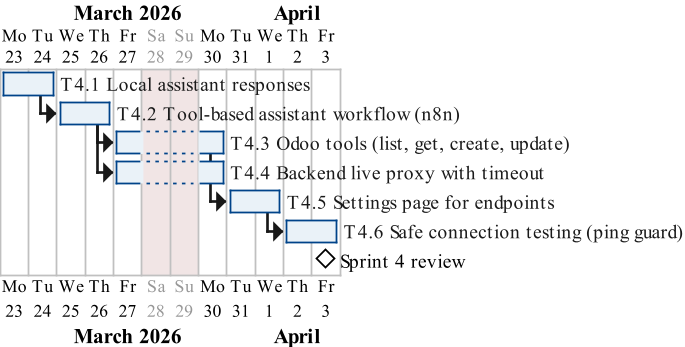
\includegraphics[width=\textwidth,height=0.42\textheight,keepaspectratio]{umls/img/gantt-sprint4.png}
\caption{Sprint 4 schedule (Gantt chart)}
\end{figure}
\figdesc{The chart organizes assistant integration, controlled CRM tools, live endpoint configuration, safe connection testing, and final validation.}

\section{Functional Analysis}\label{sumlbl:c8s3}
The assistant answers CRM questions and performs controlled actions through tools. It does not get free access to the system. It is connected to a fixed set of Odoo tools, each with a clear description: list the opportunities, read one opportunity, create an opportunity, read the CRM notes, and update a name, a phone, or an email. The assistant also follows strict output rules, so the answer is clean for the interface. The user can also configure the workflow endpoints and test the connection from the settings page.

\subsection{Use Case Diagram}\label{sumlbl:c8s3ss1}
The figure below presents the use case diagram of this sprint.

\begin{figure}[H]
\centering
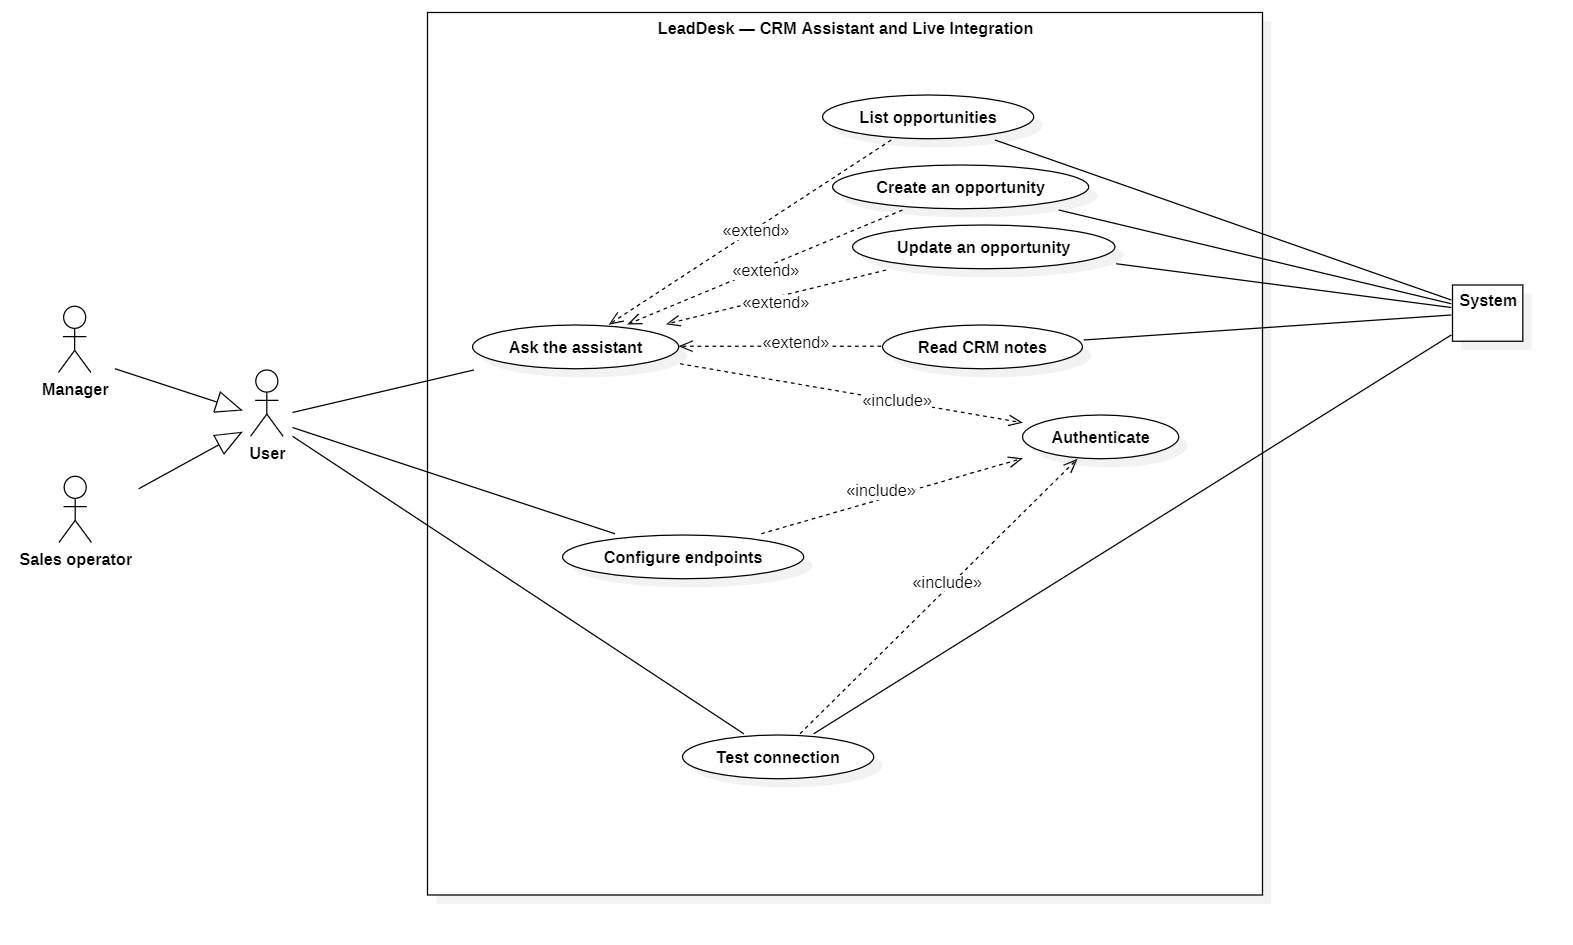
\includegraphics[width=\textwidth,height=0.9\textheight,keepaspectratio]{umls/img/uc-assistant-live.png}
\caption{Use case diagram of the assistant and live integration module}
\end{figure}
\figdesc{The diagram presents the questions and configuration actions initiated by the user and the controlled CRM services executed by the system.}

\noindent\textbf{Actor responsibilities.}
\begin{itemize}
\item \textbf{User:} asks CRM questions, requests supported opportunity operations, configures live endpoints, and starts the safe connection test.
\item \textbf{Manager:} specializes the User role and uses the assistant and live settings while supervising CRM activity and integration availability.
\item \textbf{Sales operator:} specializes the User role and uses the assistant to retrieve or maintain opportunity information during daily sales work.
\item \textbf{System:} authenticates the request, routes it through the live proxy and n8n, lets the assistant invoke only approved Odoo tools, and returns the formatted result or a clear error.
\end{itemize}

\subsection{Use Case Descriptions}\label{sumlbl:c8s3ss2}
The table below describes the use cases shown in the diagram above.

\begin{table}[H]
\centering
\small
\begin{tabularx}{\textwidth}{|p{3.6cm}|p{2.2cm}|X|}
\hline\rowcolor{TabHead}
\textbf{Use case} & \textbf{Actor} & \textbf{Description} \\
\hline
Ask the assistant & User & Send a CRM question in natural language and read a clean answer. \\
\hline
List opportunities & User & Ask the assistant to return the opportunities as cards (all of them, or a single record looked up by name or identifier). \\
\hline
Create an opportunity & User & Ask the assistant to add a new opportunity to the CRM when no duplicate exists. \\
\hline
Update an opportunity & User & Ask the assistant to change a name, a phone, or an email. \\
\hline
Read CRM notes & User & Ask the assistant to summarize the CRM notes of an opportunity. \\
\hline
Configure endpoints & User & Set the workflow endpoints used by the live integration. \\
\hline
Test connection & User & Run a safe read-only check that does not change CRM data. \\
\hline
Authenticate & System & Guard the assistant and settings actions through the backend session check. \\
\hline
\end{tabularx}
\caption{Use case descriptions for the assistant and live integration module}
\end{table}

The assistant is built around an agent connected to a small set of controlled tools. The diagram below shows this structure.

\begin{figure}[H]
\centering
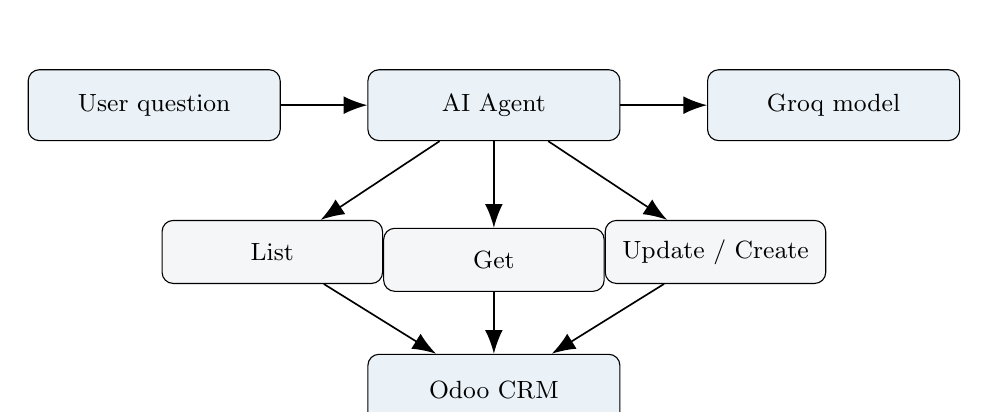
\begin{tikzpicture}[node distance=1.1cm, every node/.style={font=\small}]
\tikzset{box/.style={draw, rounded corners, fill=SoftBlue, minimum width=3.2cm, minimum height=0.9cm, align=center}}
\tikzset{tool/.style={draw, rounded corners, fill=SoftGray, minimum width=2.8cm, minimum height=0.8cm, align=center}}
\tikzset{arrow/.style={-{Latex[length=3mm]}, semithick}}
\node[box] (user) {User question};
\node[box, right=of user] (agent) {AI Agent};
\node[box, right=of agent] (model) {Groq model};
\node[tool, below left=1cm and -0.2cm of agent] (list) {List};
\node[tool, below=of agent] (get) {Get};
\node[tool, below right=1cm and -0.2cm of agent] (update) {Update / Create};
\node[box, below=2.7cm of agent] (odoo) {Odoo CRM};
\draw[arrow] (user) -- (agent);
\draw[arrow] (agent) -- (model);
\draw[arrow] (agent) -- (list);
\draw[arrow] (agent) -- (get);
\draw[arrow] (agent) -- (update);
\draw[arrow] (list) -- (odoo);
\draw[arrow] (get) -- (odoo);
\draw[arrow] (update) -- (odoo);
\end{tikzpicture}
\caption{Tool-based CRM assistant architecture}
\end{figure}
\figdesc{The architecture constrains the assistant to a defined set of CRM tools so that each read or write action remains explicit, traceable, and limited in scope.}

\section{Conceptual Modeling}\label{sumlbl:c8s4}
\subsection{Class Diagram}\label{sumlbl:c8s4ssC}
The class diagram below shows the classes involved in the assistant: the assistant with its controlled tools, and the opportunity records it reads and updates.

\begin{figure}[H]
\centering
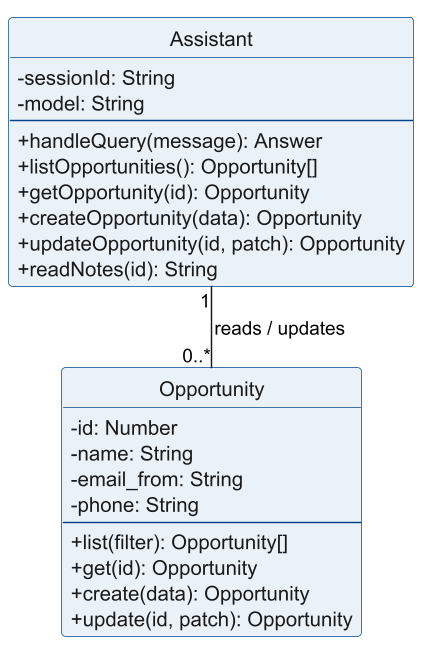
\includegraphics[width=0.8\textwidth,height=0.5\textheight,keepaspectratio]{umls/img/class-assistant.png}
\caption{Class diagram of the CRM assistant module}
\end{figure}
\figdesc{The diagram models the assistant session, user message, generated response, and controlled tool calls used to access CRM information.}

\subsection{Sequence Diagram}\label{sumlbl:c8s4ss1}
The sequence diagram below shows a full question, from the user to the displayed answer, including the live proxy and a tool call.

\begin{figure}[H]
\centering
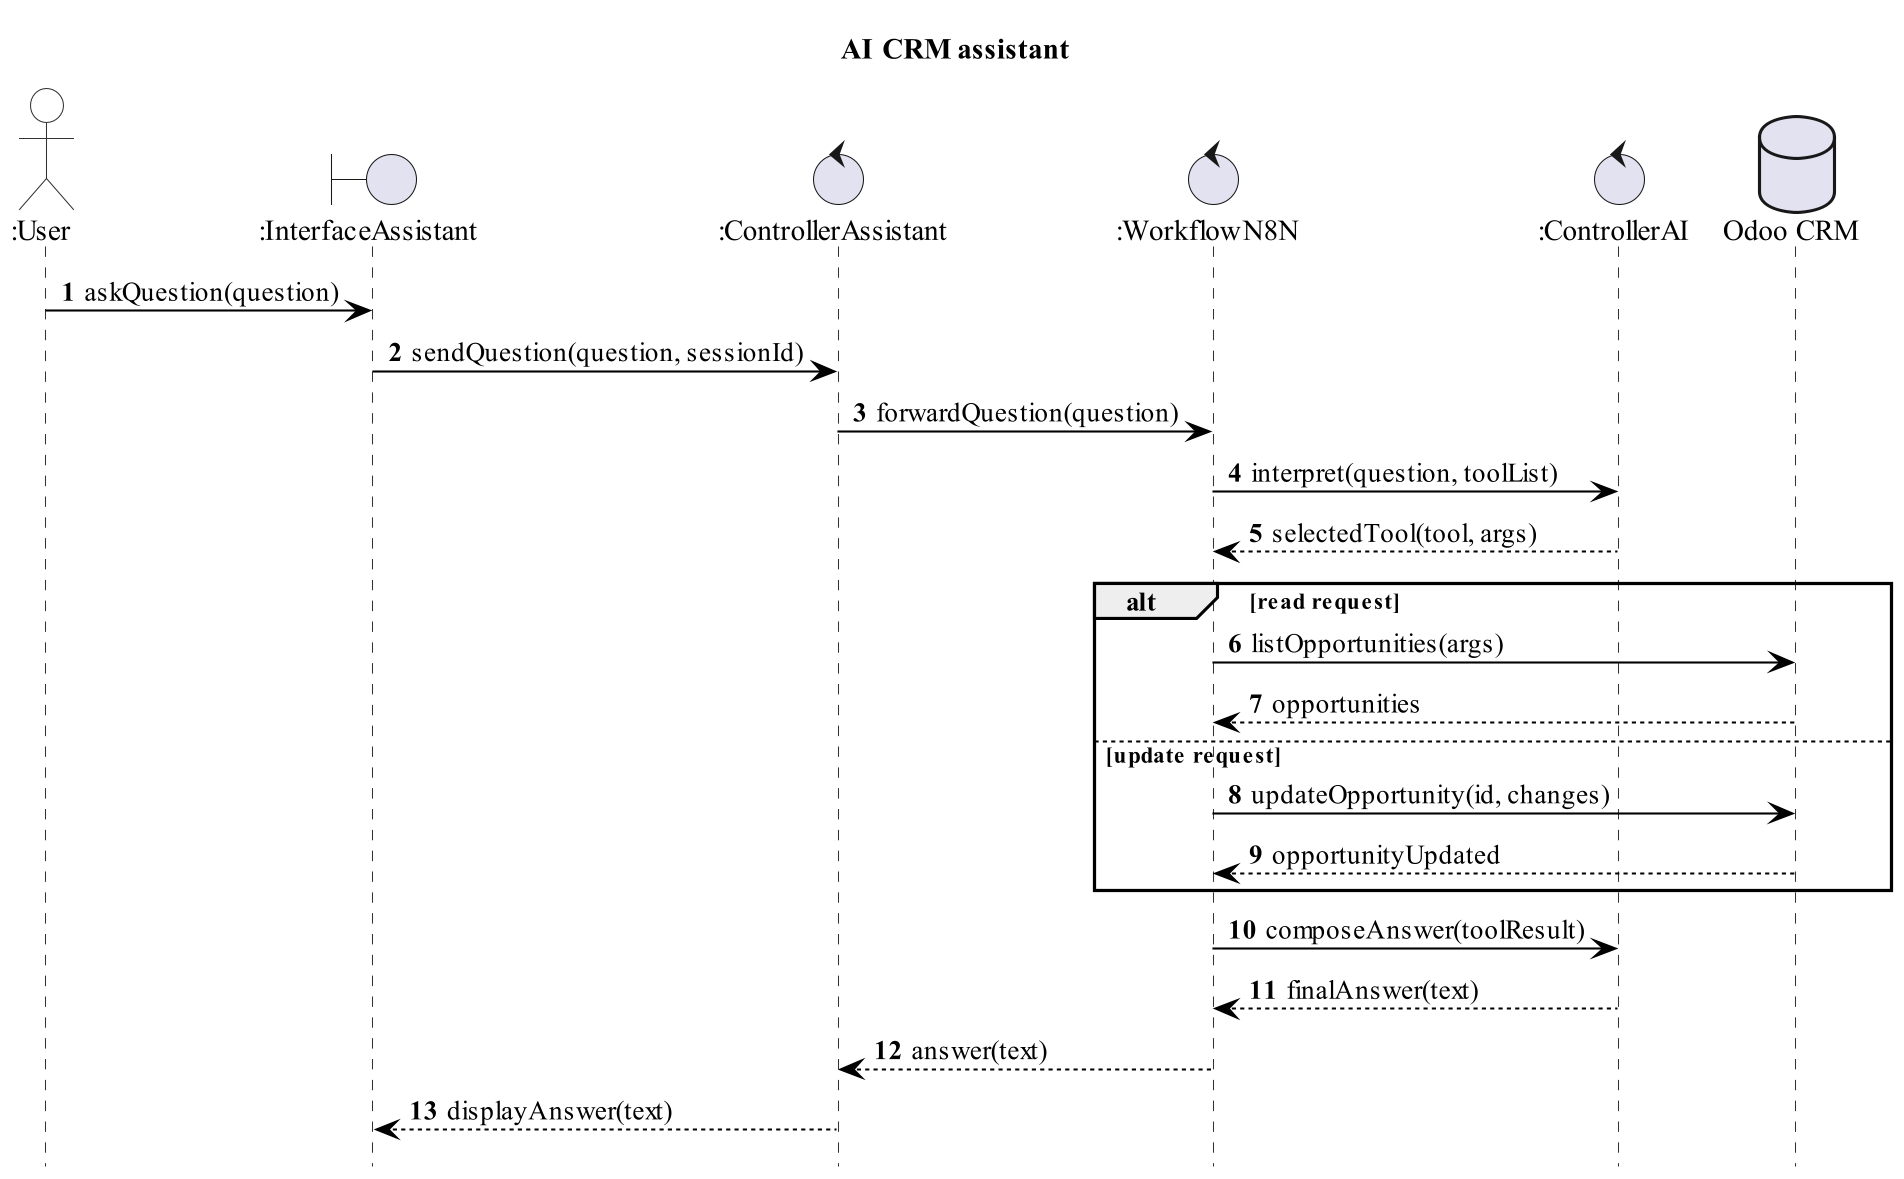
\includegraphics[width=0.92\textwidth,height=0.62\textheight,keepaspectratio]{umls/img/seq-assistant.png}
\caption{Sequence diagram of the AI assistant workflow}
\end{figure}
\figdesc{The sequence traces a natural-language question through authentication, proxy forwarding, agent reasoning, approved Odoo tool use, and response formatting.}

The settings page can also test the live connection. The sequence below shows the safe connection test, which uses the ping guard and a server-side timeout and does not modify any CRM data.

\begin{figure}[H]
\centering
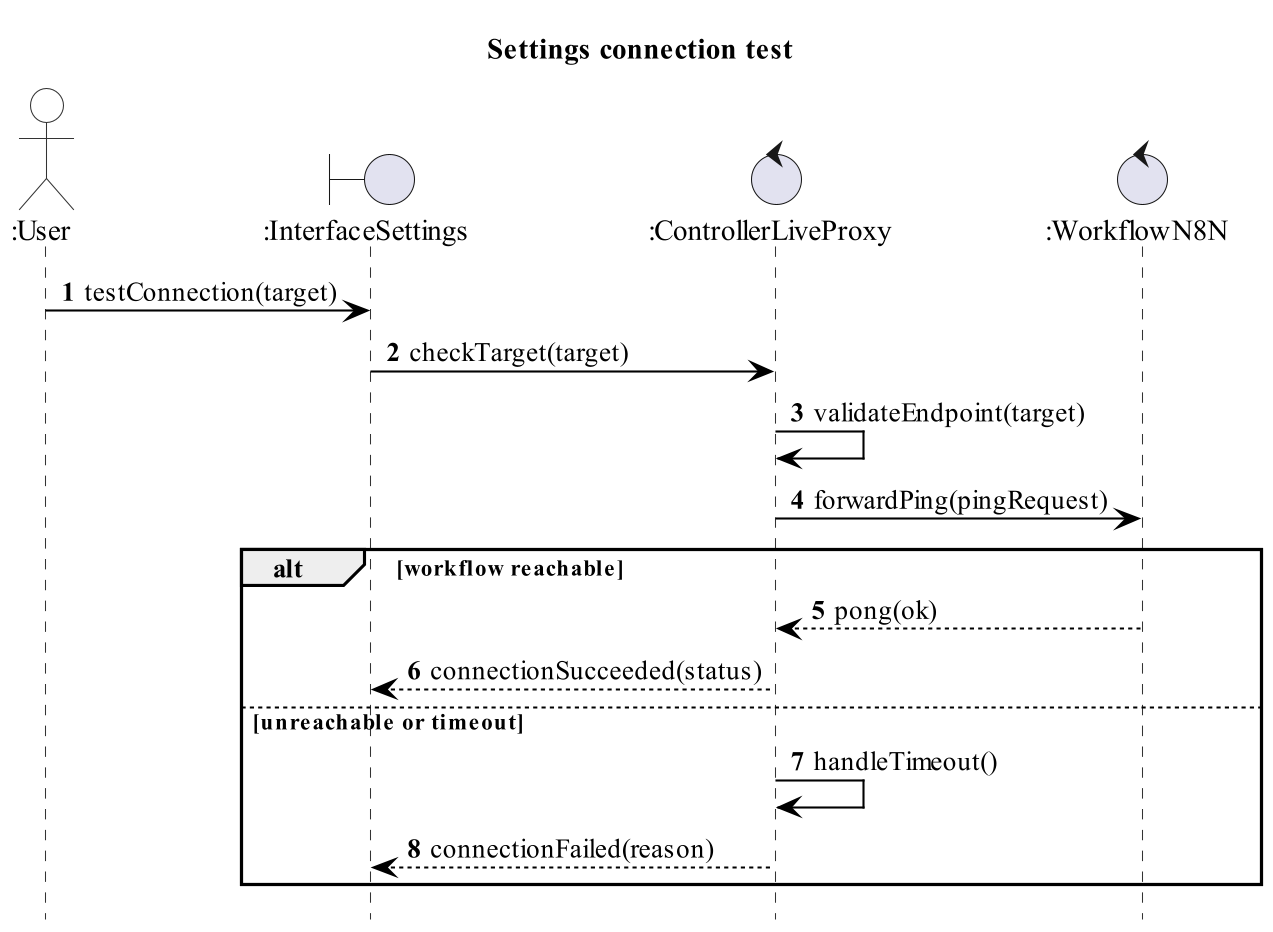
\includegraphics[width=0.92\textwidth,height=0.62\textheight,keepaspectratio]{umls/img/seq-test-connection.png}
\caption{Sequence diagram of the connection test workflow}
\end{figure}
\figdesc{The sequence shows a read-safe health check passing through the backend proxy and workflow ping guard, with a timeout preventing an indefinite wait.}


\section{Realization}\label{sumlbl:c8s5}
The live proxy is one of the most important reliability improvements in the project. Instead of letting the browser call n8n directly, the browser calls the backend on the same origin, and the backend forwards the request to n8n. This removes the CORS problems and lets the backend control the timeout, so the user gets a clear error message instead of an endless loading state. The proxy also accepts a custom endpoint only when it uses HTTP or HTTPS and belongs to the configured n8n host, which stops it from becoming an open request tool. The settings page lets the user set the endpoints and test the connection with a safe read-only ping that never writes to Odoo.

\subsection{Screenshots}\label{sumlbl:c8s5ss1}
The screenshots below show the CRM assistant, the architecture page, and the settings that control the live integration.

\shot{11-assistant.png}{CRM assistant}{This screenshot showcases the CRM assistant. The user asks a question in natural language, and the assistant answers by reading the CRM data through its connected tools.}

\shot{12-architecture.png}{Architecture page}{This screenshot showcases the built-in architecture page, which explains the layers of the platform and how a request travels from the interface to the backend, the workflows, and the CRM.}

\shot{13-settings.png}{Settings and live endpoints}{This screenshot showcases the settings page. The user configures the live workflow endpoints and runs a safe read-only connection test that never writes to the CRM.}

\section{Conclusion}\label{sumlbl:c8s6}
Sprint 4 completed the main scope of the platform. The assistant improved the usability, and the backend proxy made the live integration more stable and more secure. The next chapter presents the global testing strategy, the deployment steps, the limitations, and the validation of the final version.


\chapter{Testing, Deployment, and Validation}

\vspace{0.35cm}
{\Large\bfseries Summary}\par
\vspace{3pt}{\color{black}\hrule height 0.6pt}\vspace{0.30cm}
{\small
\chsummaryitem{9.1}{Introduction}{sumlbl:c9s1}
\chsummaryitem{9.2}{Testing Strategy}{sumlbl:c9s2}
\chsummaryitem{9.3}{Functional Tests}{sumlbl:c9s3}
\chsummaryitem{9.4}{Integration Tests}{sumlbl:c9s4}
\chsummaryitem{9.5}{Security and Reliability Tests}{sumlbl:c9s5}
\chsummaryitem{9.6}{Deployment Procedure}{sumlbl:c9s6}
\chsummaryitem{9.7}{Limitations}{sumlbl:c9s7}
\chsummaryitem{9.8}{Future Improvements}{sumlbl:c9s8}
\chsummaryitem{9.9}{Conclusion}{sumlbl:c9s9}
}
\clearpage

\section{Introduction}\label{sumlbl:c9s1}
Testing and validation are essential for a final year project. A system can hold good ideas and still fail if it is not stable in real use. This chapter presents the testing strategy used to validate LeadDesk, the deployment procedure, the limitations of the current version, and the possible improvements.

\section{Testing Strategy}\label{sumlbl:c9s2}
The testing strategy mixes manual testing, workflow execution tests, and local backend tests. Since the project is a prototype and not an industrial product, the most important goal was to validate the complete user journey. The tests therefore followed realistic actions: sign in, capture a lead, detect a duplicate, read the dashboard, generate follow-ups, and ask the assistant.

The project also separates safe tests from tests that can change data. For example, testing a connection to a workflow must not create a new opportunity. This is why the ping guard was added. The workflows that write to Odoo were tested carefully with controlled input.

\section{Functional Tests}\label{sumlbl:c9s3}
The table below presents the functional test cases run on the final application.

\begin{table}[H]
\centering
\scriptsize
\resizebox{\textwidth}{!}{%
\begin{tabular}{|p{3.7cm}|p{5.2cm}|p{4cm}|p{1.8cm}|}
\hline\rowcolor{TabHead}
\textbf{Module} & \textbf{Scenario} & \textbf{Expected behaviour} & \textbf{Result} \\
\hline
Authentication & Sign in with a valid user & The user reaches the dashboard & Passed \\
\hline
Authentication & Sign in with a wrong password & An error message is shown & Passed \\
\hline
Navigation & Open every sidebar page & The page content changes correctly & Passed \\
\hline
Lead Capture & Submit a complete customer message & Read the fields and create the record & Passed \\
\hline
Lead Capture & Submit the same lead twice & The duplicate status is shown & Passed \\
\hline
Workspace & Search by name or email & The matching records are shown & Passed \\
\hline
Dashboard & Generate the summary & The KPI summary is shown & Passed \\
\hline
Follow-Up & Run the follow-up center & The inactive leads receive draft messages & Passed \\
\hline
Assistant & Ask a count question & The assistant returns the pipeline count & Passed \\
\hline
Settings & Save the endpoints & The settings stay saved & Passed \\
\hline
\end{tabular}%
}
\caption{Functional test cases for the final application}
\end{table}

\section{Integration Tests}\label{sumlbl:c9s4}
Integration testing focused on the communication between the front end, the backend, n8n, Odoo, and the AI models. The most important point is the live path. In the live environment, the request goes from the web console to the backend live proxy, then to the n8n webhook, then to Odoo or the model, and back through a clean response to the interface.

The integration tests confirmed that the backend proxy makes the live path more stable. When n8n is unavailable, the application does not stay silent. It returns a clear message that the workflow could not be reached. When a workflow takes too long, the timeout returns a readable message. This behaviour is important for user trust.

The figure below shows the integration path followed by a live request.

\begin{figure}[H]
\centering
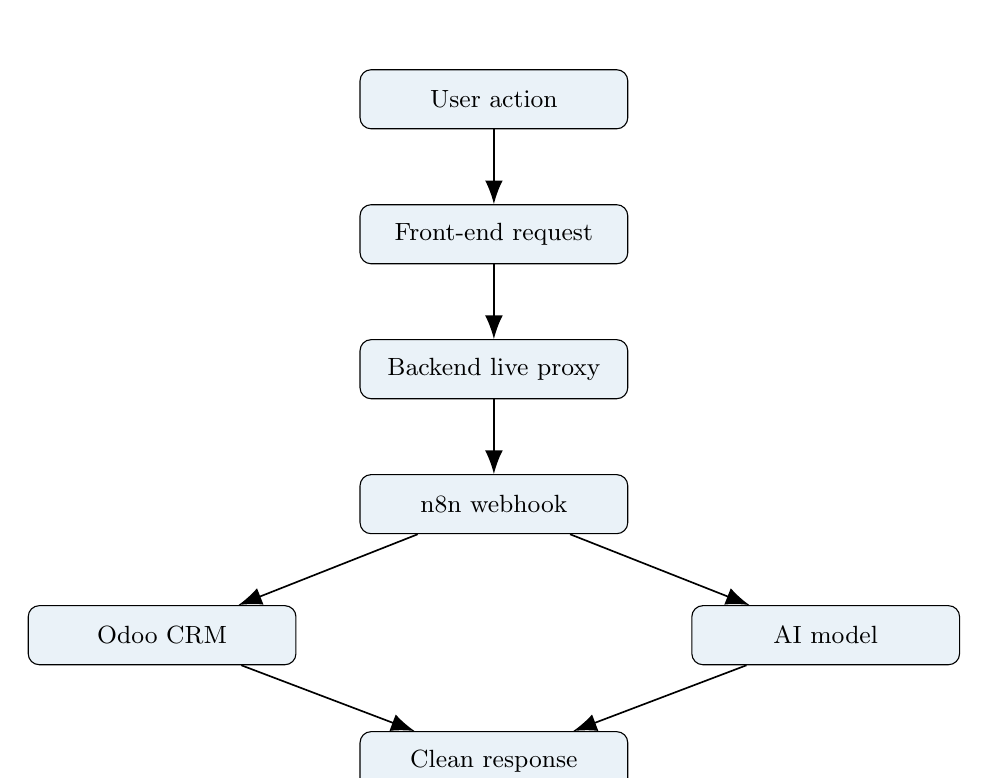
\begin{tikzpicture}[node distance=0.95cm, every node/.style={font=\small}]
\tikzset{flowstep/.style={draw, rounded corners, fill=SoftBlue, minimum width=3.4cm, minimum height=0.75cm, align=center}}
\tikzset{arrow/.style={-{Latex[length=3mm]}, semithick}}
\node[flowstep] (u) {User action};
\node[flowstep, below=of u] (f) {Front-end request};
\node[flowstep, below=of f] (b) {Backend live proxy};
\node[flowstep, below=of b] (n) {n8n webhook};
\node[flowstep, below left=0.9cm and 0.8cm of n] (o) {Odoo CRM};
\node[flowstep, below right=0.9cm and 0.8cm of n] (m) {AI model};
\node[flowstep, below=2.5cm of n] (r) {Clean response};
\draw[arrow] (u) -- (f);
\draw[arrow] (f) -- (b);
\draw[arrow] (b) -- (n);
\draw[arrow] (n) -- (o);
\draw[arrow] (n) -- (m);
\draw[arrow] (o) -- (r);
\draw[arrow] (m) -- (r);
\end{tikzpicture}
\caption{Integration path of a live request}
\end{figure}
\figdesc{The diagram follows a live request from the browser through the same-origin backend proxy to n8n and Odoo, then returns the normalized response along the same path.}

\section{Security and Reliability Tests}\label{sumlbl:c9s5}
Security testing focused on simple but important points. The passwords are never stored in clear text; they are hashed with scrypt. The backend uses bearer tokens for the sessions, and the protected routes require a valid token. The live proxy checks custom endpoints so that only the n8n host is accepted.

Reliability testing focused on failure cases. The application was tested when n8n is down, when a workflow returns unexpected text, when the assistant has no matching record, and when a customer message does not hold enough information. The expected behaviour is not to crash, but to show a clear result or a clear error.

\section{Deployment Procedure}\label{sumlbl:c9s6}
The local deployment is simple. The user installs Node.js, opens the project folder, installs the dependencies, and starts the backend. The backend then serves the application on its local port. For the live environment, n8n and Odoo must be running and the workflow endpoints must be active.

\section{Limitations}\label{sumlbl:c9s7}
The current version is a final year project prototype and not a finished production CRM. Some limitations are expected. The webhooks need stronger authentication before production use. The local database is fine for the project but should be replaced by a more robust database for a multi-user deployment. The follow-up workflow drafts messages but does not send the emails directly. The assistant handles defined CRM actions but should be extended carefully before allowing more sensitive operations.

Another limitation is AI reliability. Even with strict prompts and a temperature of zero, a model can sometimes produce unexpected output. The project reduces this risk with validation, safe defaults, and code for the numerical logic, but a production version would need extra monitoring and logging.

\section{Future Improvements}\label{sumlbl:c9s8}
Future versions can add stronger webhook authentication and per-user audit logs. The follow-up module can be connected to an email provider so that approved messages are sent directly. The dashboard can gain richer indicators such as the conversion rate and the opportunity stages. The local database can be replaced by PostgreSQL or another relational database. The assistant can also be improved with more tools and a confirmation step before it changes important data.

\section{Conclusion}\label{sumlbl:c9s9}
This chapter presented the validation of the final application. The tests confirmed that the main features work in the local environment and that the live environment is reached through a safer proxy. The project still has limitations, but it provides a solid base for a practical AI-assisted CRM automation solution.


\clearpage
\chapter*{General Conclusion}
\addcontentsline{toc}{chapter}{General Conclusion}
\markboth{GENERAL CONCLUSION}{GENERAL CONCLUSION}
This final year project set out to design and implement an AI-assisted CRM automation platform that helps a sales team manage leads more efficiently. The problem it addresses is the manual and repetitive work involved in lead capture, duplicate checking, CRM reporting, follow-up preparation, and CRM search. The proposed solution brings these operations into one web console connected to a backend, n8n workflows, Odoo CRM, and AI models.

The work produced a functional platform with a set of modules: authentication, dashboard, lead capture, duplicate detection, lead workspace, follow-up center, CRM assistant, architecture page, settings page, and live integration. The project also includes the n8n workflows for lead capture, analytics summary, smart follow-up, CRM list, and the AI assistant. The backend adds reliability features such as local persistence, authentication, a live proxy, endpoint validation, and timeout handling.

One of the main lessons of the project is that AI must be controlled when it is used in business software. The model is useful for reading information, writing summaries, drafting messages, and answering questions. Code, however, stays necessary for the calculations, the duplicate detection, the date comparisons, and the validation. The project therefore combines AI with code-based rules instead of depending only on prompts.

In conclusion, LeadDesk shows how web development, backend architecture, workflow automation, CRM integration, and artificial intelligence can be combined into one coherent software product. The current version is a solid prototype that can be extended with stronger security, production database storage, email sending, richer analytics, and a more capable assistant.


\appendix
\chapter{Additional Interface Screenshots}
This appendix gathers the interface screens that were not shown inside the sprint chapters. It keeps the visual reference complete without repeating the screenshots already presented earlier.

\shot{02-signup.png}{Sign-up screen}{This screenshot showcases the sign-up screen, where a new user creates an account with a name, an email, and a password before entering the console.}

\shot{09-workspace-detail.png}{Lead workspace: opportunity detail}{This screenshot showcases the detailed view of a single opportunity in the lead workspace, where the full captured information and the drafted follow-up are shown together.}

\chapter{User Guide}
This appendix explains how to run the platform and what each main page does. It is written in a practical way so the application can be used without confusion.

\section{Starting the Application}
The platform runs locally with Node.js. After the dependencies are installed, the backend is started and the interface opens in the browser on the local port. The same backend serves both the interface and the API, so only one server is needed. To use the live environment, n8n and Odoo are started as well, and the workflow endpoints are set on the settings page.

\section{Main Pages of the Platform}
The table below lists the main pages of the platform and what the user does on each.

\begin{table}[H]
\centering
\begin{tabularx}{\textwidth}{|p{3.6cm}|X|}
\hline\rowcolor{TabHead}
\textbf{Page} & \textbf{What the user does} \\
\hline
Dashboard & Reads the pipeline indicators and the short summary \\
\hline
Lead Capture & Pastes a customer message and gets a structured opportunity \\
\hline
Workspace & Searches the opportunities and opens a record in detail \\
\hline
Follow-Up Center & Sees inactive leads and the drafted follow-up messages \\
\hline
CRM Assistant & Asks CRM questions in natural language \\
\hline
Architecture & Reads how the layers of the system fit together \\
\hline
Settings & Sets the workflow endpoints and tests the connection \\
\hline
\end{tabularx}
\caption{Main pages of the platform and their use}
\end{table}

\section{Common Questions}
The table below answers the questions most often asked about the platform.

\begin{table}[H]
\centering
\scriptsize
\resizebox{\textwidth}{!}{%
\begin{tabular}{|p{5.2cm}|p{9cm}|}
\hline\rowcolor{TabHead}
\textbf{Question} & \textbf{Answer} \\
\hline
Why not use only Odoo? & Odoo stays the CRM system of record. The platform adds an operational layer on top of it for capture, follow-up, and assistant interaction. \\
\hline
Does the AI invent the KPI numbers? & No. The numbers are computed by code. The model only turns them into a readable summary. \\
\hline
What happens if the model returns invalid output? & The workflow and the backend include validation and safe defaults, so the application keeps working instead of crashing. \\
\hline
Why use n8n? & It makes the automation steps visible and easy to inspect and change, which is harder with hidden code-only automation. \\
\hline
What is the hardest part? & Controlling the AI behaviour and keeping the full system reliable from the interface down to Odoo. \\
\hline
\end{tabular}%
}
\caption{Common questions about the platform}
\end{table}

\chapter{Extended Test Register}
This appendix adds a more detailed test register for the final version of the project. The tests are written in a practical style and can be used during a final check before submitting the report.

\small
\begin{longtable}{|p{1.2cm}|p{2.8cm}|p{4.4cm}|p{3.8cm}|p{1.3cm}|}
\caption{Extended test register}\\
\hline
\rowcolor{TabHead}
\textbf{ID} & \textbf{Module} & \textbf{Input / action} & \textbf{Expected result} & \textbf{Status} \\
\hline
\endfirsthead
\multicolumn{5}{l}{\footnotesize\itshape Table \thetable\ -- continued from previous page}\\
\hline
\rowcolor{TabHead}
\textbf{ID} & \textbf{Module} & \textbf{Input / action} & \textbf{Expected result} & \textbf{Status} \\
\hline
\endhead
\hline
\multicolumn{5}{r}{\footnotesize\itshape continued on next page}\\
\hline
\endfoot
\hline
\endlastfoot
TR-01 & Authentication & Valid manager credentials & The dashboard opens with the manager user & Passed \\
\hline
TR-02 & Authentication & Invalid password & An error message, no session created & Passed \\
\hline
TR-03 & Sign-up & New name, email, password & The account is created with the sales role & Passed \\
\hline
TR-04 & Dashboard & Open the dashboard & The KPI cards and charts are visible & Passed \\
\hline
TR-05 & Dashboard & Generate the summary & The summary uses the KPI numbers & Passed \\
\hline
TR-06 & Capture & Complete sales message & The email, phone, intent, and priority are read & Passed \\
\hline
TR-07 & Capture & Message without an email & An empty email is accepted, no crash & Passed \\
\hline
TR-08 & Capture & Duplicate email & The duplicate is returned & Passed \\
\hline
TR-09 & Capture & Duplicate phone & The duplicate is returned & Passed \\
\hline
TR-10 & Workspace & Search an existing name & The matching row appears & Passed \\
\hline
TR-11 & Workspace & Open the details view & The full record details are visible & Passed \\
\hline
TR-12 & Follow-Up & Run inactive detection & Leads inactive for seven days or more appear & Passed \\
\hline
TR-13 & Follow-Up & Lead without an email & No repeated email selection problem & Passed \\
\hline
TR-14 & Assistant & Ask to list the opportunities & The records are shown in cards & Passed \\
\hline
TR-15 & Assistant & Ask a count question & The number of opportunities is returned & Passed \\
\hline
TR-16 & Assistant & Ask for an unknown record & A not-found message is shown & Passed \\
\hline
TR-17 & Settings & Save an endpoint value & The value stays saved & Passed \\
\hline
TR-18 & Settings & Test a safe workflow & A pong or a clear connection result & Passed \\
\hline
TR-19 & Live proxy & n8n stopped & A clear unreachable message & Passed \\
\hline
TR-20 & Live proxy & Slow workflow & A timeout message after the set delay & Passed \\
\hline
TR-21 & Security & Reach a protected route without a token & An unauthorized response & Passed \\
\hline
TR-22 & Security & Password storage & The password is stored as a scrypt hash & Passed \\
\hline
TR-23 & Environment & Switch from Local to Live & The data source changes without a crash & Passed \\
\hline
TR-24 & Environment & Live unavailable & The user sees an honest error message & Passed \\
\hline
TR-25 & Architecture page & Open the architecture section & The explanation and diagram are visible & Passed \\
\hline
\end{longtable}
\normalsize

\chapter*{Bibliography}
\addcontentsline{toc}{chapter}{Bibliography}
\markboth{BIBLIOGRAPHY}{BIBLIOGRAPHY}
\begin{enumerate}[label={\textup{[\arabic*]}}, leftmargin=1.2cm]
\item Odoo Documentation, CRM and developer documentation.
\item n8n Documentation, Workflow automation, webhook nodes, and integrations.
\item Express.js Documentation, Node.js web application framework.
\item MDN Web Docs, HTML, CSS, JavaScript, Fetch API, and browser APIs.
\item Node.js Documentation, crypto module, HTTP server concepts, and runtime environment.
\item NeDB Documentation, embedded datastore usage in Node.js applications.
\item Ollama Documentation, local large language model runtime.
\item Groq Documentation, hosted language model API and supported models.
\item Ken Schwaber and Jeff Sutherland, The Scrum Guide.
\item Scrum.org, ``What is Scrum?'' learning module.
\item International Institute of Technology academic guidelines for final year project reporting.
\end{enumerate}

\clearpage
\chapter*{Webography}
\addcontentsline{toc}{chapter}{Webography}
\markboth{WEBOGRAPHY}{WEBOGRAPHY}
\begin{enumerate}[label={\textup{[W\arabic*]}}, leftmargin=1.5cm]
\item Odoo, ``CRM documentation,'' \url{https://www.odoo.com/documentation/19.0/applications/sales/crm.html}.
\item Google, ``Google Sheets,'' \url{https://workspace.google.com/products/sheets/}.
\item Salesforce, ``What is CRM?'', \url{https://www.salesforce.com/crm/what-is-crm/}.
\item Multisoft, ``What is an automation tool and how do you choose the right one?'', \url{https://www.multisoft.se/en/kunskapsbank/what-is-an-automation-tool-and-how-do-you-choose-the-right-one/}.
\item Scrum.org, ``What is Scrum?'', \url{https://www.scrum.org/resources/what-scrum-module}.
\item Microsoft, ``Visual Studio Code documentation,'' \url{https://code.visualstudio.com/docs}.
\item Git, ``Git documentation,'' \url{https://git-scm.com/doc}.
\item OpenJS Foundation, ``Node.js,'' \url{https://nodejs.org/en}.
\item Express, ``Express web framework,'' \url{https://expressjs.com/}.
\item Meta Open Source, ``React,'' \url{https://react.dev/}.
\item Vite, ``Vite guide,'' \url{https://vite.dev/guide/}.
\item MDN Web Docs, ``HTML: HyperText Markup Language,'' \url{https://developer.mozilla.org/en-US/docs/Web/HTML}.
\item MDN Web Docs, ``CSS: Cascading Style Sheets,'' \url{https://developer.mozilla.org/en-US/docs/Web/CSS}.
\item MDN Web Docs, ``JavaScript,'' \url{https://developer.mozilla.org/en-US/docs/Web/JavaScript}.
\item n8n, ``Workflow automation documentation,'' \url{https://docs.n8n.io/}.
\item PostgreSQL Global Development Group, ``About PostgreSQL,'' \url{https://www.postgresql.org/about/}.
\item Docker, ``Docker Desktop documentation,'' \url{https://docs.docker.com/desktop/}.
\item NeDB project repository, \url{https://github.com/louischatriot/nedb}.
\item MDN Web Docs, ``REST,'' \url{https://developer.mozilla.org/en-US/docs/Glossary/REST}.
\item JSON.org, ``Introducing JSON,'' \url{https://www.json.org/json-en.html}.
\item Ollama, ``Ollama documentation,'' \url{https://docs.ollama.com/}.
\item Groq, ``Groq developer documentation,'' \url{https://console.groq.com/docs/overview}.
\item Connexant, company website, \url{http://connexant.net/}.
\item Microsoft, ``Microsoft Excel,'' \url{https://www.microsoft.com/en-us/microsoft-365/excel}.
\item Odoo, ``Odoo CRM,'' \url{https://www.odoo.com/app/crm}.
\item Zapier, company website, \url{https://zapier.com/}.
\item Make, company website, \url{https://www.make.com/}.
\end{enumerate}


\includepdf[pages=1,fitpaper=true]{backpage-filled.pdf}

\end{document}
